%
%  $Description: Author guidelines and sample document in LaTeX 2.09/2e$
%
%  $Author: Priit Ruberg$
%  $Date: 2015/02/09 $
%  $Revision: 2.5 $
%
%  Translated to English 2017/03/10 by Chris Raastad
%
\documentclass[a4paper,12pt]{article} %Document class definition and text size settings
%
%Packages can be explored in more details: https://www.ctan.org/pkg/PACKAGE_NAME?lang=en
%
\usepackage{graphicx} %Allow using graphics in the text
\usepackage[top=2.5cm, bottom=2.5cm, left=3cm, right=3cm]{geometry} %Set the page margins
\usepackage{titlesec} %Package for title style
\usepackage[table]{xcolor} %make a colorful table
\usepackage{longtable} %Package so tables can be longer than one page
\usepackage{multirow} %Package so table cells can span multiple rows
\usepackage[colorinlistoftodos]{todonotes} %Package so you can add nice TODO marks in your paper with \todo{TODO text...}
\usepackage{cite} %For Bibtex

%colors for risk categorization table
\definecolor{pool1}{HTML}{FF3333}
\definecolor{pool2}{HTML}{FF9933}
\definecolor{pool3}{HTML}{FFFF33}
\definecolor{pool4}{HTML}{99FF33}

\usepackage{hyperref}
% \usepackage{url} %Package in order to nicely use URLs
\usepackage{float} %Package to improves interface for defining floating objects like figures and tables

\usepackage[english, estonian]{babel} %Specifies possible languages of the document: English, Russian, and Estonian
	\addto\captionsestonian{\def\refname{\centerline{References}}} %Changes references name and makes it center
	\addto\captionsestonian{\def\listfigurename{\centerline{List of figures}}} %Changes drawing list name and makes it center
	\addto\captionsestonian{\def\listtablename{\centerline{List of tables}}} %Changes table list name makes it center
	\addto\captionsestonian{\def\contentsname{\centerline{Table of contents}}}
\usepackage[T2A,T1]{fontenc} %Font encodings for Russian and Estonian letters
\usepackage[utf8]{inputenc} %use UTF8 decodings

\usepackage{tocloft} %Control table of contents, tables, etc.
%\setlength\cftparskip{-2pt}
%\setlength\cftbeforechapskip{0pt}

\usepackage{amssymb} %For square itemized listss
\renewcommand{\labelitemi}{\tiny$\blacksquare$} %For square itemized lists


\usepackage{caption} %Needed to customise captions for tables and figures
\captionsetup{labelsep=period} %Set table and figure caption name to be separated with text with a period

\usepackage{verbatimbox} %To put program code in the center using Verbatim

\titlelabel{\thetitle.\quad} %Adds periods to the end of titles

\usepackage{times} %Sets font to Times New Roman
\usepackage{fancyhdr} %Allows more control of headers and footers
\setlength{\parindent}{0cm} %Set paragraph indentation to zero %consider removing this...

\usepackage{setspace} %Allows setting spacing between lines
% \onehalfspacing %Set spacing to 1.5x LaTeX
\linespread{1.25} %Set spacing to 1.5x like MS word

\usepackage{parskip}
%\setlength{\parskip}{1.5\baselineskip} % default for parskip
%\hangindent=0.7cm

\hyphenation{põhi-tekstis üliõpilas-kood lehe-küljed joonda-takse} %Correcting incorrect hyphenation (?)

\usepackage{eurosym}
\usepackage{quoting} %for quoting format
\quotingsetup{vskip=0pt} %for no vertical whitespace around quotings

% a bunch of stuff to make paragraph act as a subsubsubsection and numbered and formatted correctly
\usepackage{titlesec}
\setcounter{secnumdepth}{4}
\titleformat{\paragraph}
{\normalfont\normalsize\bfseries}{\theparagraph}{1em}{}
\titlespacing*{\paragraph}
{0pt}{3.25ex plus 1ex minus .2ex}{1.5ex plus .2ex}

\usepackage{enumerate} %for more control of ordered lists

\usepackage[none]{hyphenat} %kill hyphenation
\usepackage{ragged2e} % for nice justification in abstracts

\usepackage{amsmath}
\usepackage{amsfonts}
\usepackage{amssymb}

\usepackage{graphicx}
\graphicspath{ {images/} }

% --- new commands ---

% creates hyperref using the name of a reference
\newcommand{\hypernameref}[1]{\hyperref[#1]{\nameref{#1}}}

% creates a hyperref in form "Table #" for a table
\newcommand{\hypertableref}[1]{\hyperref[#1]{Table \ref{#1}}}

% creates a hyperref in form "Figure #" for a figure
\newcommand{\hyperfigureref}[1]{\hyperref[#1]{Figure \ref{#1}}}

% creates a hyperref in form "Section #" for a section
\newcommand{\hypersectionref}[1]{\hyperref[#1]{Section \ref{#1}}}

% make font look like code
\def\code#1{\texttt{#1}}

% ability to add line breaks in tables (by making a new table...)
% http://tex.stackexchange.com/questions/2441/how-to-add-a-forced-line-break-inside-a-table-cell
\newcommand{\specialcell}[2][c]{%
  \begin{tabular}[#1]{@{}l@{}}#2\end{tabular}}

\begin{document}
\selectlanguage{english}

%------------------------------ENGLISH TITLE PAGE---------------------------------
\thispagestyle{fancy} %Page will include header and footer
\renewcommand{\headrulewidth}{0pt} %Remove header horizontal line
\renewcommand{\footrulewidth}{0pt} %Remove footer horizontal line
\headheight = 57pt %Set header heght (with regards to compiler suggestion)
\footskip = 11pt %Footer space
\headsep = 0pt %Decrease header and text line spacing distance to zero

\chead{ %Place the following text header to the center
 \textsc{\begin{Large} %Make the following text have big letters
	TALLINN UNIVERSITY OF TECHNOLOGY\\
	\end{Large}}
	Faculty of Information Technology\\
	Department of Computer Engineering
}
\vspace*{7 cm} %Make the page beginning and text line spacing correspond to the width

\begin{center} %Text centered
ITC70LT\\[0cm]
Christopher David Raastad\\
\begin{LARGE}
\textsc{Security Analysis of the Euro 2.0 Digital Currency Prototype\\}
\end{LARGE}
Master thesis\\[2cm]
\end{center}

\begin{flushright} %Align text to the right
Alexander Horst Norta\\[0cm]
PhD\\[0cm]
Associated Professor\\[0cm]
\end{flushright}

\cfoot{Tallinn, Estonia 2017} %Add location and year to the header
%\renewcommand{\headrulewidth}{0pt} %Remove the footer horizontal line
\pagebreak %End of page

%------------------------------TIITELLEHT EESTI KEELES---------------------------------
\selectlanguage{estonian}
\thispagestyle{fancy} %Leht sisaldab päist ja jalust
\renewcommand{\headrulewidth}{0pt} %Eemaldab päisest horisontaalse joone
\renewcommand{\footrulewidth}{0pt} %Eemaldab jalusest horisontaalse joone
\headheight = 57pt %Paneb paika päise laiuse (vastavalt kompilaatori soovitusele)
\footskip = 11pt %Jaluse ruum
\headsep = 0pt %Vähendab päise ja teksti vahelise kauguse nullini

\chead{ %Paigutab järgneva teksti päises keskele
 \textsc{\begin{Large} %Tekst suurtähtedega ja suuremaks
	tallinna tehnikaülikool\\
	\end{Large}}
	Infotehnoloogia teaduskond\\
	Arvutitehnika instituut
}
\vspace*{7 cm} %Tekitab lehe alguse ja teksti vahele tühja ala vastava laiusega

\begin{center} %Tekst keskele
ITC70LT\\[0cm]
Christopher David Raastad\\
\begin{LARGE}
\textsc{Euro 2.0 Digitaalne Valuuta Prototüübi Turvalisusanalüüs\\}
\end{LARGE}
Magister\\[2cm]
\end{center}

\begin{flushright} %Joondab teksti paremale
Alexander Horst Norta\\[0cm]
PhD\\[0cm]
Dotsent\\[0cm]
\end{flushright}

\cfoot{Tallinn, Estonia 2017} %Lisab asukoha ja kuupäeva jalusesse
%\renewcommand{\headrulewidth}{0pt} %Eemaldab päisest horisontaalse joone
\pagebreak %Lehe lõpp


%----------------------------LIST OF TODOS----------------------------------
\listoftodos
\newpage

%---------------------------AUTHOR DECLARATION-------------------------
\selectlanguage{english}
\section*{\begin{center}
 Author’s declaration of originality
\end{center}}
I hereby certify that I am the sole author of this thesis. All the used materials, references to the literature and the work of others have been referred to. This thesis has not been presented for examination anywhere else.

Author: Christopher David Raastad

May 8th 2017
\pagebreak

%---------------------------ABSTRACT---------------------------------
\section*{\begin{center}
Abstract
\end{center}}

Digital money in the form of cards, bank accounts, and online payments has been around for the last few decades. The cryptocurrency Bitcoin emerged as a completely new paradigm of storing and transferring value outside of the regulations and governments of the traditional financial system. The blockchain distributed ledger consensus technology powering Bitcoin inspired similar cryptocurrency clones, specialized use cases, and the creation of a general purpose distributed application computing platform Ethereum. Despite the innovations in value transfer, cryptocurrencies have a very niche use in daily transactions outside the circle of enthusiasts. The problem is the lack of incentive for users and merchants alike to hold all of their assets in a cryptocurrency. Significant cost and friction is associated with moving funds in and out of cryptocurrencies through exchanges and payment processors as well as the risk of wildly fluctuating exchange rates. The Euro 2.0 Foundation presents a fiat backed, fully regulated, government backed digital currency to alleviate these shortcomings. This thesis presents a security analysis of the proposed Euro 2.0 digital currency prototype. We present the features and architecture of the Euro 2.0 digital currency, a fusion of traditional client server components, Estonia ID card authentication, and Ethereum smart contract decentralized distributed computing platform. Then we present a change analysis of the impact of the Euro 2.0 digital on the stakeholders including users, merchants, banks, and government. Finally we present an information system security risk analysis based on the OCTAVE Allegro methodology of key information assets user money, Ethereum admin keys, and user identity. From the security analysis we present suggestions and mitigation strategies of the biggest risks of a hybrid centralized and decentralized Euro 2.0 digital currency system.

\todo[inline]{Fill in English abstract thesis details \ldots}

The thesis is in English and contains [pages] pages of text, [chapters] chapters, [figures] figures, [tables] tables.

\pagebreak

%-----------------------------ANNOTATSIOON-----------------------------------
\selectlanguage{estonian}
\section*{\begin{center}
Annotatsioon
\end{center}}

\sloppy Digitaalne raha on kaartide, pangakontode ja internetimaksete kujul olemas olnud juba aastakümneid. Krüptoraha Bitcoin kujundas täiesti uue paradigma väärtuste hoidmisele ja ülekannete tegemisele väljaspool traditsiooniliste finantssüsteemide regulatsioone ning valitsust. Plokiahela abil loodi ühtse tehnoloogiaga avalik raamatupidamisregister, olles inspireeritud sarnaste krüptorahade kloonidest, erilistest kasutamisjuhtudest ja üldotstarbelise rakenduste arvutamise platvormi Ethereum loomisest. Vaatamata väärtuste ülekannete protsesside innovatsioonile on krüptoraha väljaspool entusiastide ringe igapäevakasutuses siiski niši staatuses. Probleem tuleneb sellest, et kasutajatel ning kaupmeestel puuduvad stiimulid kõiki oma varasid krüptovaluutas hoida. Lisaks valuutakursside suurtele kõikumistele seostatakse krüptoraha märkimisväärseid kulusid ja huvide vastuolusid raha liigutamisega krüptovaluutasse ja tagasi valuutavahetuste ja maksete töötlemise protsesside käigus. Euro 2.0 Sihtasutus esitleb täielikult reguleeritud, ametlike volitustega ja valitsuse poolt toetatud digitaalvaluutat, millega soovitakse kõiki neid puudusi leevendada. Käesolev magistritöö esitab kavandatava Euro 2.0 digitaalvaluuta prototüübi turvalisusanalüüsi. Töös on välja toodud Euro 2.0 digitaalvaluuta omadused ja ülesehitus,  traditsiooniliste kliendiserverite lülide, Eesti ID-kaardi autentimise ning Ethereum targa lepingu detsentraliseeritud hajusandmetöötluse platvormi integratsioon. Järgmisena on esitatud analüüs Euro 2.0 digitaalvaluuta mõjust huvigruppidele, hõlmates kasutajaid, kaupmehi, panku ja valitsust. Lõpetuseks tuuakse välja infosüsteemi turvariskid toetudes OCTAVE Allegro kasutajate varade olulise teabe metoodikale, Ethereumi haldajate võtmete ja kasutajate identideedi analüüsile. Turvalisusanalüüsi põhjal esitatakse soovitused ja leevendamise strateegiad hübriid-tsentraliseeritud ja detsentraliseeritud Euro 2.0 digitaalvaluutasüsteemi suurimatele riskidele.

\todo[inline]{Täitke eesti keele annotatsiooni lõputöö detailid \ldots}

Lõputöö on kirjutatud inglise keeles ning sisaldab teksti [lehekülgede arv] leheküljel, [peatükkide arv] peatükki, [jooniste arv] joonist, [tabelite arv] textit.

\pagebreak

%---------------------ABBREVIATIONS AND GLOSSARY OF TERMS---------------------
\selectlanguage{english}
\section*{\begin{center}
Table of abbreviations and terms
\end{center}}

\begin{tabular}{p{3 cm} p{10cm}}
	BTC & Bitcoin currency code\\
	AML & \textit{Anti Money Laundering}, processes implemented by Financial Institutions to hinder money laundering and comply with regulation\\
	CTF & \textit{Counter Terrorist Financing}, processes implemented by Financial Institutions to hinder terrorist financing and comply with regulation\\
	KYC & \textit{Know Your Customer}, proccesses of Financial institution to identify and verify customers' identities to aid AML and CTF\\
	ISSRM & \textit{Information Systems Security Risk Management} \\
	SK & \textit{Sertifitseerimiskeskus} (Certification Center), SK ID Solutions AS, the only Certificate Authority (CA) in Estonia for the Estonian ID card system. \\
	LDAP & \textit{Lightweight Directory Access Protocol} hosted by SK \\
	API & \textit{Application Programming Interface}, describing communicating between two servers \\
	UX & \textit{User Experience}
\end{tabular}

\pagebreak

%----------------------------TABLE OF CONTENTS----------------------------------
\tableofcontents
\newpage

%----------------------LIST OF DRAWINGS-------------------------------
\listoffigures
\pagebreak

%----------------------LIST OF TABLES---------------------------------
\listoftables
\pagebreak

%-----------------------------CHAPTER 1 - INTRODUCTION-------------------------------
\section{Introduction} \label{sec:1}

Payments today are the laggard of the information age. While emails can be sent instantly for free anywhere in the world, money is either slow and/or expensive to move digitally. Bank transfers can take days, only work during business hours, and have high fees across borders. Card payments are instant, but subject merchants to high fees and chargeback risks. Paypal brought convenient payments to the web, but at a high cost to accept payments and move funds internationally. Fintech companies like Venmo and Square can create the illusion of fast payments, but still take days to settle in the background with the potential chargeback risks. This cost comes from the highly regulated centralized financial payments systems with little economic incentive to reduce fees. A usable digital currency would greatly alleviate this friction in transferring value that theoretically costs the economy an estimated 1\% of GDP annually \cite{kaarmann2013cost}.

Bitcoin was the first successful implementation of a decentralized digital currency. Nakamoto's peer to peer digital cash system completely sidestepped the existing financial system\cite{nakamoto2008bitcoin}. Its clever proof of work consensus protocol, economic incentives for nodes to maintain the network, pseudo anonymity, and irreversible transactions implemented on the public ledger Blockchain technology has been called ``the next technological revolution''\todo{citation, probably from Blockchain Revolution}. Hundreds of Altcoins followed Bitcoin's lead borrowing from the Blockchain technology to implement other flavors of cryptocurrency and digital asset management. Despite the rapid growth of the cryptocurrency ecosystem, everyday payments are a niche use case for digital currencies, which are more commonly used for investment and financial speculation\cite{Khairuddin:2016:EMB:2851581.2892500}. Merchants accepting Bitcoin payments are in fact immediately converting funds to a fiat currency for a non negligible fee. Bitcoin Exchanges are high cost gatekeepers between the cryptocurrency and financial systems.

What is missing today are incentives for parties on both sides of payments to hold assets end to end in digital currency. The cost and friction of moving between two financial systems, crypto and fiat, eliminates the perceived benefits of crypto currencies. The Euro 2.0 project aims to implement fiat currency on digital currency technology and reduce friction by eliminating unnecessary financial intermediaries. The unanimous adoption of Estonian ID card in Estonia and the Ethereum distributed application platform make a prototype system possible. This thesis introduces the Euro 2.0 system, its impact on stakeholders in the payments, and assesses the security, scalability, and privacy risks of the implementation to determine whether this system can in fact reasonably support a national digital currency.

\subsection{Existing Body of Knowledge} \label{ssec:1.1}
\todo[inline]{Existing body of knowledge to gap detection}


\subsection{Research Questions} \label{ssec:1.2}

This thesis explores the feasibility of the Euro 2.0 digital currency by answering the following research question:
\begin{quoting}
	\textbf{RQ: }\textit{How do we assure that the proposed Euro 2.0 digital currency does not have any major security, scalability, or privacy flaws compromising the usefulness of the monetary system?}
\end{quoting}

In which we explore in sub research questions:
\begin{quoting}
\textbf{RQ1: }\textit{How do we describe the relevant features needed for analysis of the Euro 2.0 digital currency?}
\end{quoting}
\begin{quoting}
\textbf{RQ2: }\textit{How does adoption of Euro 2.0 digital currency impact the relationship with money for key stakeholders: users, merchants, governments, and financial institutions?}
\end{quoting}
\begin{quoting}
\textbf{RQ3: }\textit{How do we assess the security and privacy risks of Euro 2.0 digital currency system and potential impact on stakeholders?}
\end{quoting}

Answering \textbf{RQ} will result in one of two possible outcomes:
\begin{itemize}
	\item The Euro 2.0 system is free from significant risks in functioning as a digital monetary system.
	\item The Euro 2.0 system has one or more serious risks that need to be addressed before significant adoption.
\end{itemize}

In order to do a risk analysis, the key features of the Euro 2.0 system need to be identified and implementation details described by answering \textbf{RQ1}. Following a clear specification of the system, \textbf{RQ2} explores the current and future relationship with money of key stakeholders after adoption of Euro 2.0. This exploration of the stakeholders' relationship with money grounds the analysis of the impact of realized risks uncovered in \textbf{RQ3}. The severity and likelihood of realized risks to the monetary system lead to an answer to the original research question \textbf{RQ}.

\subsection{Research Methods} \label{ssec:1.3}
The thesis utilizes methods from design science and Information Systems Security Risk Management (ISSRM) to approach the research questions. The main contributions are:
\begin{itemize}
	\item Presentation of the Euro 2.0 digital currency prototype
	\item Change analysis of stakeholders' transition to Euro 2.0 money transfer
	\item Security Risk analysis of the Euro 2.0 prototype
	\item Recommendations how to mitigate risks
\end{itemize}

\subsection{Structure of the Thesis} \label{ssec:1.4}

\hypernameref{sec:2} will give an overview of the existing body of knowledge needed to understand the remaining chapters including: traditional finance, Bitcoin, Tether, Ethereum, Estonia ID card, and security analysis methodology. \hypernameref{sec:3} will describe the motivation, features, smart contracts, and implementation architecture of the Euro 2.0 system and prototype needed for analysis. \hypernameref{sec:4} will analyze the impact of Euro 2.0 on stakeholders using change analysis to better understand the socio-technical impact of the proposed digital currency. In \hypernameref{sec:5} we will perform a security risk analysis of the proposed Euro 2.0 prototype implementation OCTAVE Allegro, an ISSRM based security analysis methodology. Finally \hypernameref{sec:6} will summarize the thesis, answer the research question, and suggest future avenues of research.

\pagebreak

%--------------------CHAPTER 2 - BRIDGE-----------------
\section{Chapter 2: Bridge of Knowledge} \label{sec:2}

\todo[inline]{Write Chapter 2}

\subsection{Traditional Finance System}

\subsection{CryptoCurrencies and Payments}
Existing crypto currencies not great for payments...

\subsubsection{Bitcoin}

\subsubsection{Tether}

\subsubsection{Anonymity vs. Regulation vs. Trust}

\subsection{Ethereum} \label{ssec:2:ethereum}

Ethereum generalizes Blockchain technology as a decentralized computing platform for building distributed applications. Ethereum is used to implement the decentralized component of Euro 2.0, providing the main account balance and state data and functionality described in \hypersectionref{ssec:3.4}. \hypersectionref{sssec:2:ethereum:platform} gives an overview of the necessary details of the Ethereum platform and \hypersectionref{sssec:2:ethereum:soliditySmartContracts} outlines the key points of the Solidity Smart Contracts programming language used later in the thesis.

\subsubsection{Ethereum Platform} \label{sssec:2:ethereum:platform}

The core of Ethereum is the \textit{Ethereum Virtual Machine} (EVM), which functions as a decentralized general purpose computing platform with Turning complete scripting functionality. Ethereum is formally specified in Wood's \textit{Ethereum: A Secure Decentralised Generalised Transaction Ledger}\cite{yellowpaper}, also know as the ``Yellowpaper'' functioning as a ``technical bible'' of the Ethereum platform. The Yellowpaper, although very detailed and thorough, is too low level of a formal specification to be digestible as an introduction to the platform. Buterin's Ethereum Whitepaper, \textit{A Next-Generation Smart Contract and Decentralized Application Platform}\cite{whitepaper}, is a high level introduction to the platform suitable for understanding the key decentralized concepts of Euro 2.0.  Anderson et al. compare Namecoin, Peercoin, and Ethereum to Bitcoin, looking at factors such as Blockchain disk size and client bootstrapping security, and present the results of a crawler on the Ethereum Blockchain looking at contract usages and Zombie contracts\cite{Anderson2016NewKO}.

\paragraph*{Accounts}

Ethereum state is held in objects called \textit{accounts}. An account is composed of the following fields:

\begin{itemize}
	\item \textit{nonce} - a counter used to make sure each transaction can only be processed once
	\item \textit{balance} - amount of Ether in the account
	\item \textit{contract code} - the code associated with this account, if present
	\item \textit{storage} - storage space for this account
\end{itemize}

An Ethereum account is named with a 20 byte address. This address is the \code{Keccak-256} hash of a public key of a private generated from an Elliptic Curve Digital Signature Algorithm. Accounts come in two flavors: \textit{Externally Controlled Accounts} and \textit{Contract Accounts}. Externally controlled accounts are controlled by private keys of users outside of Ethereum and can be used to send messages by creating and signing transactions. Contract account code is executed upon a received messages to the address. This executed code can read and write to local storage, send other messages, and also create contracts. Both types of accounts store a balance of \textit{Ether}, the currency of Ethereum, which can be used as a store of value and as fee for miners to execute EVM code. Ether is produced by miners as an output of producing blocks in a Proof-of-Work mechanism. Unlike bitcoin, Ether doesn't have a capped total supply, but is anticipated to be produced at the same rate of Ether being lost to unaccessible accounts where the private key is lost or unknown.

\paragraph*{Messages and Transactions}

Messages and transactions in Ethereum are the same construct. A \textit{Transaction} refers to a signed message from an externally owned Ethereum account with the following fields:

\begin{itemize}
	\item Recipient Ethereum address of the message
	\item Signature identifying the sender
	\item Amount of Ether transferred from the sender to the recipient
	\item Optional data field accessible by smart contract
	\item \code{STARTGAS} value in Ether, the maximum amount of fee a given transaction is allowed to execute
	\item \code{GASPRICE} value in Ether, the fee the sender pays per computational step
\end{itemize}

Transactions are persisted on the blockchain. Account code will be executed upon receipt of a message. Gas allows for a Turing complete scripting language by creating economical disincentive for accidental or intentional denial of service attacks through infinite loops or expensive computations. Each computational step has a fee in a multiple of \code{GASPRICE} and when greater or equal to transaction specified \code{STARTGAS} has been executed, the computation fails with all execution changes rollback. Blocks of transactions also have a dynamic gas limit to the total computational expense of an entire block of transactions.

Messages refer to those originating from a contract \code{CALL} opcode and not by an external actor. These are not persisted on the blockchain and are only virtual objects in the Ethereum execution environment of nodes on the network. Messages contain the following fields:

\begin{itemize}
	\item Sender Ethereum address of the message
	\item Recipient Ethereum address of the message
	\item Amount of ether to transfer with the message
	\item Optional data field
	\item \code{STARTGAS} value in Ether delegated to the message from calling contract original gas
\end{itemize}

Limited top level \code{STARTGAS} prevents contracts from calling in infinite recursive loops.

\paragraph*{Ethereum State Transition Function}

Unlike Bitcoin's unspent transaction output (\textit{UTXO}), Ethereum employs an account model of system state. The Ethereum state $S$ represents the state of all addresses, balances, contracts, and data in the Ethereum. Given a transaction $TX$ the new Ethereum state $S'$ is computed by the state transaction function $APPLY(S,TX) -> S'$ and does the following according to the Ethereum Whitepaper\cite{whitepaper}:

\begin{itemize}
	\item Check if transaction is valid, signature is valid, and nonce matches sender account nonce; if not throw an error.
	\item Calculate transaction fee as \code{STARTGAS * GASPRICE}, determine the sending address from the signature, subtract the fee from the sender's account balance, and increments the sender's nonce. If there is not enough balance, throw an error.
	\item Initialize \code{GAS = STARTGAS}, and take off a certain quantity of gas per byte to pay for the bytes in the transaction.
	\item Transfer the transaction value from the sender's account to the receiving account. If the receiving account does not yet exist, it is created. If the receiving account is a contract, run the contract's code either to completion or until the execution runs out of gas.
	\item If the value transfer failed because the sender had insufficient balance or the code execution ran out of gas, revert all state changes except the payment of the fees, and add the fees to the miner's account.
	\item Otherwise, refund the fees for all remaining gas to the sender, and send the gas fees consumed to the miner.
\end{itemize}

State is calculated and stored identically on every node in the network for all transactions.

\paragraph*{Ethereum Code}

Ethereum code is fundamentally a low-level, stack-based, byte code language referred to as the ``EVM code''. Ethereum code is usually written in high level languages such as python based Serpent\cite{serpent} or javascript based Solidity, which is described in \hypersectionref{sssec:2:ethereum:soliditySmartContracts}, and then compiled to EVM bytecode. Code executes until an error is thrown, runs out of gas, or a \code{STOP} or \code{RETURN} statement is executed. Persistence capabilities include a last-in-first-out (LIFO) \textit{stack} in which values can be pushed and popped, an infinitely expandable byte array \textit{memory}, or contract \textit{storage}, a key value store which persists after computation has finished (unlike the memory or stack). Executing code also has access to the value, sender, and data of an incoming message and can return a byte array of data as an output.

\paragraph*{Events}
Events are a space optimized, searchable, storage of predefined conditions in contracts described formally in the Yellowpaper\cite{yellowpaper}. This is analogous to logs in the traditional computing. These logs are not usable like contract storage in future Ethereum computations, but provide searchable records of the past usable in Ethereum applications.

\paragraph*{Blockchain and Mining}

Ethereum has a proof-of-work mining mechanism, like Bitcoin, to economically incentivize miner nodes to maintain the global state of Ethereum network for Ether rewards. Miners compete to solve a cryptographic puzzle to produce valid blocks of transactions. The hash of the previous block is an input to a new block, hence forming a Blockchain record of transactions. In the process of mining, the block validation process executes the EVM code for all contracts involved in transactions. This implies that all EVM code is being executed simultaneously by all nodes in the network and all contract data is public and shared on the network. Blocks are mined in Ethereum at an average rate of ten to fifteen seconds unlike, the rate of ten minutes of Bitcoin. The security of the network lies in the difficulty of producing valid blocks, with valid cryptographic proof-of-work puzzle, and valid state transition faster than new blocks of honest nodes.

\subsubsection{Solidity Smart Contracts} \label{sssec:2:ethereum:soliditySmartContracts}

\paragraph*{Data}

\paragraph*{Functions}

\paragraph*{Modifiers}

Throw Exceptions

\subsection{Estonia ID Card}


\subsection{ISSRM Framework}

Information System Security Risk Management (ISSRM) is a broad field with \textit{``over 200 practitioner-oriented risk management methods and several academic security modeling frameworks available"}\cite{Dubois2010}. Duboi et al. build a unified domain model of ISSRM by surveying and categorizing risk management standards, information security and information technology standards, risk management methodologies, and security frameworks, as well as the state of the art of security modeling languages. This serves as a useful source of representative security risk analysis frameworks to choose from.

Ahmed and Matulevi\v{c}ius explore eliciting security requirements earlier in business process modeling by introducing security risk oriented patterns\cite{Ahmed:2014:SBP:2588915.2589308}. The goal is to ``align business processes and security requirements elicited using security risk-oriented patterns'' to mitigate security risks. This gives a good contextual framework for thinking through a security analysis on business processes.

Uzunov and Fernandez give a deeply technical overview of security patterns of distributed systems\cite{Uzunov:2014:EPL:2588915.2589309}. They first survey threat patterns, pattern-based threat taxonomies, and architectural contexts for the threat patterns. Then they provide a list first level security threat patterns and second level meta-security threat patterns to see further analysis. Then they construct a specialized taxonomy of security threats for distributed and peer to peer systems. The ideas presented are useful input for the Euro 2.0. security risk analysis in \hypersectionref{sec:5}.

From the review of ISSRM frameworks, \textit{OCTAVE Allegro} was chosen as the simplest framework allowing a strait forward risk analysis of the Euro 2.0 proccesses using a seven step methodology\cite{CaralliIntroducingOCTAVE2007}:

\begin{itemize}
	\item \textit{Step 1 - Establish Risk Measurement Criteria}
	\item \textit{Step 2 - Develop an Information Asset Profile}
	\item \textit{Step 3 - Identify Information Asset Containers}
	\item \textit{Step 4 - Identify Areas of Concern}
	\item \textit{Step 5 - Identify Threat Scenarios}
	\item \textit{Step 6 - Identify Risks}
	\item \textit{Step 7 - Analyze Risks}
	\item \textit{Step 8 - Select Mitigation Approach}
\end{itemize}

We use inspiration from security patterns of from the other two papers as input for the OCTAVE Allegro risk analysis. We chose not to undergo formal modeling or complicated modeling software, as complexity explodes when applied to a complicated system like Euro 2.0, without any benefits of the time invested.

\pagebreak

%--------------------CHAPTER 3-----------------
\section{Chapter 3} \label{sec:3}

\subsection{Introduction} \label{ssec:3.1}
This chapter introduces the Euro 2.0 digital currency system. The contents of this section are based from a prototype developed by the Euro 2.0 Foundation as a non profit initiative. All the original code is accessible in Github under the MIT License as indicated in \hyperref[ssec:a.1]{Appendix A.1}. The chapter answers the following research question:

\begin{quoting}
\textbf{RQ1:} \textit{How do we describe the relevant features needed for risk analysis of the Euro 2.0 digital currency?}
\end{quoting}

Which is broken down into the following sub-questions:
\begin{quoting}
	\textbf{RQ1.1: }\textit{What are the features of the Euro 2.0 digital currency?}
\end{quoting}{
\begin{quoting}
	\textbf{RQ1.2: }\textit{What are the decentralized components?}
\end{quoting}{
\begin{quoting}
	\textbf{RQ1.3: }\textit{What are the centralized components?}
\end{quoting}
\begin{quoting}
	\textbf{RQ1.4: }\textit{How do the decentralized and centralized work together to provide the features?}
\end{quoting}

Answering \textit{RQ1} lays the groundwork for further analysis in \hypernameref{sec:4} and \hypernameref{sec:5}. \hypersectionref{ssec:3.2} will briefly go through the motivation behind the Euro 2.0 digital currency system. \hypersectionref{ssec:3.3} will give an overview of the system architecture and features currently implemented answering \textit{RQ1.1}. \hypersectionref{ssec:3.4} will give an overview of the decentralized components built on the Ethereum platform answering \textit{RQ1.2}. \hypersectionref{ssec:3.5} will give an overview of centralized components built with traditional software development architecture answering \textit{RQ1.3}. Finally \hypersectionref{ssec:3.6} will briefly describe how the centralized and decentralized components work together to fulfill the features of \hypersectionref{ssec:3.2} answering \textit{RQ1.4}.

\subsection{Euro 2.0 Motivation} \label{ssec:3.2}

The idea of Euro 2.0 originated in 2014 from Kristo Käärmann's blogpost \textit{Government Backed Bitcoin}\cite{kaarmann2014government}. Following the success of Bitcoin, he saw an opportunity for a payments settled on a Government backed cryptocurrency, \textit{EuroCoin}, pegged one to one to real world Euro counterpart. Paypal cofounder Max Levchin supports the same idea, \textit{``I am confident that there will be a form of settlement that will be a crypto-currency''}\cite{pando2014levchin}. Bitcoin's short term fluctuations, functioning both as a commodity and a currency, in value make it unreasonable for end to end holdings in a fiat based economy. Removing financial intermediaries in payments reduces the costs of transactions.

Even some governments have expressed interests in digital currency. The Swedish central bank debated whether to become the first to issue digital currency as a response to the country's move away from cash\cite{milne2016sweden}. The UK government pushed for a ``Call for Information'' on digital currencies in order to assess risks\cite{nermin2014ukcall} that was later responded by Citi bank's global Treasury and Trade Services (TTS) Technology and Innovation Team with a suggestion for government to create its own digital currency\cite{spaven2015ukcurrency}:

\begin{quoting}
	\textit{``The greatest benefits of digital currencies can be realised through the government issuing a digital form of legal tender. This currency would be less expensive, more efficient and provide greater transparency than current physical legal tender or electronic methods.''}
\end{quoting}

Following the rise in popularity of Ethereum, in mid 2016, another blogpost by Käärmann \textit{The future of money may be in the ether}\cite{kaarmann2016ether} described the rough idea of the system. I describe Euro 2.0 as solving the business problem:

\begin{quoting}
	\textit{How do I build a system to digitally store and transact fiat currency without a centralised for-profit financial intermediary conveniently, trustfully, and securely while satisfying government regulations?}
\end{quoting}

From this business problem derives the key pillars of Euro 2.0:

\begin{enumerate}
	\item Fiat Backed
	\item Decentralised Accounts and Transactions
	\item Identities of all Users
	\item Convenient Conversion of Fiat to and from Digital Euro
	\item Government can control monetary supply
	\item Features for Law Enforcement and AML
\end{enumerate}

\textit{Fiat Backed} (1) provides monetary stability to the system and builds trust with users and merchants to keep assets in the digital format. This eliminates the issue of constantly fluctuating daily value between real world and digital assets seen in crypto currencies today.

\textit{Decentralised Accounts and Transactions} (2) comes from the need of an impeccable record and process of transacting value that no centralised party can modify in a database. This is the key benefit and usecase of distributed ledger technology.

\textit{Identities of all Users} (3) builds trust in the system for users, merchants, and governments. If everyone is identified, any transaction can be legally ramified (assuming legislation arises supporting distributed ledger records in the court). The strong identity of Estonian ID card is a perfect fit for a digitally identifying mechanism and the main driver of the first prototype.

\textit{Convenient Conversion of Fiat to and from Digital Euro} (4) makes it easy for users to gradually start using the digital currency from existing financial infrastructure. At first this exchange gateway can be a private financial institution, similar to Tether\cite{tether2016whitepaper}, with a proof of reserve of the one to one Euro backing. Ideally this conversion service is hosted by the central bank itself to limit the number of financial intermediaries.

\textit{Government can control monetary supply} (5) follows from the ideal scenario of (4), the central bank can issue new money directly into the digital monetary system without a real world euro counterpart.

\textit{Features for Law Enforcement and AML} (6) is the most controversial aspect of the system. Bitcoin was made to sidestep the direct control of any third party, including government\cite{nakamoto2008bitcoin}. Euro 2.0 needs to be regulated from the start with full support of governments, which require means of necessary intervention that typically happen today via cooperation with traditional financial institutions.

\subsection{Euro 2.0 Features} \label{ssec:3.3}

The following section describes the main features of the Euro 2.0 system. Features are enumerated with the label \textbf{XY\#} where:
\begin{itemize}
	\item \textbf{X} is an abbreviation of the domain of the feature, described in the \hypernameref{sssec:3.3:domains} section
	\item \textbf{Y} is client, admin, or server. Client is a user of the system, admin is some superuser with special permissions, and server is some centralized or decentralized server infrastructure
	\item \textbf{\#} is the number of a feature for a given \textbf{XY}
\end{itemize}

Features are implemented with a combination of decentralized and centralized components described in \hypersectionref{ssec:3.4} and \hypersectionref{ssec:3.5} respectively.

\subsubsection{Domains} \label{sssec:3.3:domains}

\hypertableref{tab:domains} gives an overview of the domains of Euro 2.0 used to group features described in later sections.

\begin{center}
\begin{tabular}{ | l | c | p{10cm} | }
 \hline
 Domain & Abbr. & Description \\
 \hline
 \textbf{Account} & A & mechanism of storage of value in the system
 \\ \hline
 \textbf{Identity} & I & features linking real life human identity to users
 \\ \hline
 \textbf{Transaction} & T & mechanism of transfer of value in the system
 \\ \hline
 \textbf{Reserve} & R & features regarding the exchange of value between traditional Euro (EUR) in the financial system and digital Euro (EUR2)
 \\ \hline
 \textbf{Enforcement} & E & features for government regulators and law enforcement to police the system for misuse and AML
 \\ \hline
 \textbf{Convenience} & C & features for improving user experience and expanding use cases
 \\ \hline
\end{tabular}
\end{center}
\captionof{table}{Domains of Euro 2.0}
\label{tab:domains}

% TODO: I'm not sure if this table is actually relevant anymore
% \hypertableref{tab:centVsDecent} gives an overview of the distribution of centralised and decentralised domains of the Euro 2.0 system.
%
% \begin{center}
% \begin{tabular}{ |c|c| }
%  \hline
%  Centralised & Decentralised \\
%  \hline
%  Identity & Account \\
%  Reserve & Transaction \\
%  Enforcement & Network \\
%  Convenience & \\
%  \hline
% \end{tabular}
% \end{center}
% \captionof{table}{Centralised vs. Decentralised Domains of Euro 2.0}
% \label{tab:centVsDecent}

\subsubsection{Entities} \label{sssec:3.3:entities}

\hypertableref{tab:entities} clarifies key data entities used throughout the description of features.

\begin{center}
\begin{tabular}{ | p{3cm} | p{12cm} | }
 \hline
 Entity & Description
 \\ \hline\hline
 Address & Ethereum externally controlled address (i.e. public key) holding EUR2 and Ether
 \\ \hline
 Key & Ethereum address private key needed to make transactions (EUR2 or Ether) for an address
 \\ \hline
 Account & All verified Ethereum addresses for an ID
 \\ \hline
 Account Balance & Sum of total balance of EUR2 in an account
 \\ \hline
 ID & Estonian ID code of an individual (citizen, resident, e-resident)
 \\ \hline
 ID Name & Name of person associated with an Estonian ID Code
 \\ \hline
 EUR & Euro currency in an Estonian bank account
 \\ \hline
 EUR2 & Euro currency in the Euro 2.0 digital form, balance of an address in the Euro 2.0 Ethereum contract
 \\ \hline
 Wallet & Client program (app or mobile web) used as an interface to Euro 2.0 system, accessible keys to addresses
 \\ \hline
 Wallet Password & Password used to encrypt and decrypt local wallet
 \\ \hline
 Backup Password & Password used to encrypt and decrypt keys and address to send to backup server
 \\ \hline
 Designator account & Account collecting seized funds
 \\ \hline
\end{tabular}
\end{center}
\captionof{table}{Euro 2.0 Entities}
\label{tab:entities}

\subsubsection{Roles} \label{sssec:3.3:roles}

\begin{center}
\begin{tabular}{ | p{3cm} | p{12cm} | }
 \hline
 Role & Description
 \\ \hline\hline
 CryptoFiat Master & Ethereum address (public / private key) to master contract
 \\ \hline
 Approver & Ethereum address (public / private key) entitled to approver operations
 \\ \hline
 Reserve Bank & Ethereum address (public / private key) entitled to reserve operations and funds
 \\ \hline
 Enforcer & Ethereum address (public / private key) entitled to to enforcer operations
 \\ \hline
 Designator & Ethereum address (public / private key) entitled to designator operations
 \\ \hline
\end{tabular}
\end{center}
\captionof{table}{Euro 2.0 Roles}
\label{tab:roles}

\subsubsection{Processes} \label{sssec:3.3:processes}

\hypertableref{tab:processes} clarifies different processes used throughout the description of features.

\begin{center}
\begin{tabular}{ | p{3cm} | p{12cm} | }
 \hline
 Process & Description
 \\ \hline\hline
 Approval & Link Ethereum address with the an Estonian ID number via ID card certificate verification. Allow Ethereum address to send EUR2.
 \\ \hline
 Freeze & Stop address from sending EUR2.
 \\ \hline
 Close & Stop address from receiving EUR2.
 \\ \hline
 Seize & Remove EUR2 from an address and send them to the designator account.
 \\ \hline
 Name checks & AML PEP and Sanction list check on real name of person.
 \\ \hline
\end{tabular}
\end{center}
\captionof{table}{Euro 2.0 Processes}
\label{tab:processes}

\subsubsection{Account Features} \label{sssec:3.3:accounts}

Client
\begin{itemize}
	\item \textbf{AC1} - Create address
	\item \textbf{AC2} - View account balance
\end{itemize}

Server
\begin{itemize}
	\item \textbf{AS1} - Aggregate account balance
\end{itemize}

The account features allow users of store balance of EUR2. The requirement is an Ethereum public and private key pair created in \textbf{AC1}. Viewing account balance is taking the sum of all addresses under ownership of the user's private keys. A server aggregation is needed for retrieving the balances and resolving delegated balances described later.

\subsubsection{Identity Features} \label{sssec:3.3:identity}

Client
\begin{itemize}
	\item \textbf{IC1} - Approve address
\end{itemize}

Server
\begin{itemize}
	\item \textbf{IS1} - Check external source for valid ID
	\item \textbf{IS2} - Approve address
	\item \textbf{IS3} - Save ID number to address mapping
	\item \textbf{IS4} - Look up ethereum address by ID
\end{itemize}

In order for an address to transact EUR2, it needs to be approved, that is linked with an identity. The server here plays a critical role in approving the address by checking a client approval request (\textbf{IC1}) with an external source (\textbf{IS1}) then both approving this address on the blockchain (\textbf{IS2}) and saving this mapping (\textbf{IS3}) for use in other components (\textbf{IS4}).

\subsubsection{Transaction Features} \label{sssec:3.3:transactions}

Client
\begin{itemize}
	\item \textbf{TC1} - Send EUR2 to an address
	\item \textbf{TC2} - Send EUR2 to an ID
	\item \textbf{TC3} - Receive EUR2 to an address
	\item \textbf{TC4} - Receive EUR2 to an ID
	\item \textbf{TC5} - Send EUR2 to a EUR bank account
\end{itemize}

Server
\begin{itemize}
	\item \textbf{TS1} - Resolve ID to an address
	\item \textbf{TS2} - Escrow EUR2 to an ID
	\item \textbf{TS3} - Release escrow EUR2 to an address for an ID
	\item \textbf{TS4} - Execute valid EUR transaction
	\item \textbf{TS5} - Execute valid EUR2 transaction
\end{itemize}

The transaction features are the heart of the EUR2 system. What differentiate Euro 2.0 from other cryptocurrencies is the ability to easily send funds amongst digital (EUR2) and real (EUR) euros. \textbf{TC1} and \textbf{TC3} allow a user to transact EUR2 directly with the Ethereum decentralised system using ethereum addresses. \textbf{TC2} and \textbf{TC4} allow a user to conveniently send EUR2 to a human being via their ID code using the centralised identity infrastructure (\textbf{IS4}). Funds sent to an ID that does not yet have an Ethereum address will have EUR2 held to a new ethereum address in Escrow (\textbf{TS2}) and then later released and transferred to an address created and approved by the receiver (\textbf{TS3}). \textbf{TS5} provides the infrastructure to execute EUR2 transactions for \textbf{TC1} through \textbf{TC4}. A centralised party needs to provide the mediation gateway (\textbf{TS4}) allowing a user to send EUR2 to a EUR bank account (\textbf{TC5}).

\subsubsection{Reserve Features} \label{sssec:3.3:reserve}

Client
\begin{itemize}
	\item \textbf{RC1} - Convert EUR to EUR2
	\item \textbf{RC2} - Convert EUR2 to EUR
	\item \textbf{RC3} - Proof of reserve
\end{itemize}

Admin
\begin{itemize}
	\item \textbf{RA1} - Assign reserve bank address
	\item \textbf{RA2} - Manage reserve bank account
\end{itemize}

Server
\begin{itemize}
	\item \textbf{RS1} - Resolve address from ID of received EUR transaction
	\item \textbf{RS2} - Create EUR2
	\item \textbf{RS3} - Destroy EUR2
\end{itemize}

The reserve features allow convenient conversion between EUR and EUR2. The reserve process for converting from EUR to EUR2 is to to receive a EUR bank transaction with an individuals ID (\textbf{RS1}), create EUR2 (\textbf{RS2}) of the equivalent amount, resolve the ID to an ethereum address (\textbf{TS1}), and send this to the address for the ID (\textbf{TS5}).  Likewise the process from converting EUR2 to EUR is receiving a EUR2 transaction (\textbf{RC1}), destroy the EUR2 (\textbf{RS3}), and send a bank transfer of the equivalent amount in EUR (\textbf{TS4}). Finally there is admin feature to assign the reserve EUR2 address to make conversions (\textbf{RA1}) and actually perform manage the banking operations on the bank account (\textbf{RA2}).

\subsubsection{Enforcement Features} \label{sssec:3.3:enforcement}

Admin
\begin{itemize}
	\item \textbf{EA1} - Freeze account
	\item \textbf{EA2} - Seize account funds to designator's address, closing the account
	\item \textbf{EA3} - Assign enforcement
	\item \textbf{EA4} - Assign designator
	\item \textbf{EA5} - Set designator address
	\item \textbf{EA6} - View name check and analysis data
\end{itemize}

Server
\begin{itemize}
	\item \textbf{ES1} - Name checks on ID names
	\item \textbf{ES2} - Create database of transactions with ID
\end{itemize}

The enforcement features allow law enforcement to do their job that would be traditionally be done via financial institutions. Law enforcement can freeze (\textbf{EA1}) and seize (\textbf{EA2}) funds to the designator address (\textbf{EA5}). Admin controls exist to assign the role of enforcer (\textbf{EA3}) and designator (\textbf{EA4}). Finally automatic processes in the server need to perform name checks on all users of the system (\textbf{ES1}) and create a database of identities and transactions (\textbf{ES2}) to be usable by some analysts (\textbf{EA6}).

\subsubsection{Convenience Features} \label{sssec:3.3:backup}

The convenience features are not necessarily central to a functioning and compliant fiat and digital monetary system, but are quite useful to increase the usefulness and usability barrier. They are quite important to consider in a security analysis, hence listed here.

\paragraph{Wallet Security}
Client
\begin{itemize}
	\item \textbf{CC1} - Encrypt wallet
	\item \textbf{CC2} - Decrypt wallet
\end{itemize}

Since private keys are stored locally on a user's device, they should be encrypted (\textbf{CC1}) with some password when not in use and decrypted (\textbf{CC2}) when needed for signing transactions.

\paragraph{Key Backup}

Client
\begin{itemize}
	\item \textbf{CC3} - Encrypt keys for addresses
	\item \textbf{CC4} - Create a challenge question
	\item \textbf{CC5} - Send addresses, keys, and challenge to backup server for an ID
	\item \textbf{CC6} - Retrieve addresses and keys from backup server for an ID with challenge answer
	\item \textbf{CC7} - Decrypt keys for addresses
\end{itemize}

Server
\begin{itemize}
	\item \textbf{CS1} - Save encrypted addresses and keys for an ID
	\item \textbf{CS2} - Check challenge answer
	\item \textbf{CS3} - Load encrypted addresses and keys for an ID
\end{itemize}

Since keys are stored locally, if not backed up, they can be easily lost with the device. Euro2.0 provides a centralised convenience feature to back up these keys for an ID and secured by a challenge question. The user can encrypt their keys with a password (\textbf{CC3}), create a challenge question (\textbf{CC4}), send the addresses, encrypted keys, and challenge to the server (\textbf{CC5}) to be saved (\textbf{CS1}). The user can then retrieve the addresses and encrypted keys for an ID from the server (\textbf{CC6}) by providing the correct challenge answer checked by the server (\textbf{CS2}) (\textbf{CS3}), and finally the keys can be decrypted by the user (\textbf{CC7}).

\paragraph{Transfer Info}

Client
\begin{itemize}
	\item \textbf{CC8} - Encrypt copies of transfer details for sender and receiver
	\item \textbf{CC9} - Save transfer details for a transaction hash
	\item \textbf{CC10} - Load transfer details for a transaction hash
	\item \textbf{CC11} - Decrypt transfer details for sender or recipient
\end{itemize}

Server
\begin{itemize}
	\item \textbf{CS4} - Save transfer details for a transaction hash
	\item \textbf{CS5} - Load transfer details for a transaction hash
\end{itemize}

Transfer info features provide extra information to transfers only visible to sender and receiver. First a sender of a transaction encrypts two copies of the transfer details, one with the sender's public key and the other with the recipient's private key (\textbf{CC8}). Then these can be saved to the transfer info server with the transaction's hash (\textbf{CC9} and \textbf{CS4}). Then these details can be loaded from the server (\textbf{CS5}) by the sender or receiver from the server (\textbf{CC10}) and decrypted with their respective private key (\textbf{CC11}).

\paragraph{Account Recovery}

Client
\begin{itemize}
	\item \textbf{CC12} - Set address recovery address
	\item \textbf{CC13} - Recover address funds
\end{itemize}

Server
\begin{itemize}
	\item \textbf{CS6} - Execute address funds recovery transaction and close account
\end{itemize}

Account recovery features offer some protection from accidentally losing keys to an address. A user can set a very trusted address, a friend or close relative, with the able to recover funds (\textbf{CC12}). This trusted party at any time can perform the funds recovery and withdraw all of the account's funds to their account with their key (\textbf{CC13}) executed by the server (\textbf{CS6}).

\paragraph{Delegated Transfers - Send without Ether}

Client
\begin{itemize}
	\item \textbf{CC13} - Execute EUR2 transaction with EUR2 fee without gas
\end{itemize}

\begin{itemize}
	\item \textbf{CS7} - Fulfill delegated EUR2 transaction and claim EUR2 fee
\end{itemize}

Finally, this convenience feature eliminates the side effect of using Ethereum, consuming gas (ether) in transactions. A trusted third party, the wallet server in this case, can execute transactions on behalf of the sender (\textbf{CC13}) and take the fee in EUR2 cents instead of ether (\textbf{CS7}). This requires only the trusted third party to have Ether and the user can only worry about EUR2.

\subsection{Decentralized Components} \label{ssec:3.4}

This section walks through the decentralized components of the Euro 2.0 system on the Ethereum distributed applications platform. The main container of code deployment is the \textit{Contract}. Once deployed, the contract is on the Blockchain forever processing messages (transactions) sent to it unless an optional destroy function is implemented and called. All function calls and data modifications are irreversible and publicly visible while being executed on the 1000s of computers on the Ethereum network maintaining the Ethereum Blockchain. Thus we describe the implementation of the contracts in detail, since there is an of the code, once deployed, and is important in the security analysis considerations.

The decentralized contracts are comprised of of the main administrator contract (\textit{CryptoFiat}), shared contracts (\textit{Constants}, \textit{Relay}, \textit{Data}, \textit{InternalData}), and the upgradable subcontracts providing functionality to the system (\textit{Accounts}, \textit{Approving}, \textit{Reserve}, \textit{Enforcement}, \textit{AccountRecovery}, \textit{Delegation}). These decentralized contracts function as gateways to the shared decentralized data of the Euro 2.0 system used together with centralized components and client explained in \hypersectionref{ssec:3.5} to fulfill the features, described in \hypersectionref{ssec:3.6}.

\todo[inline]{Diagram with inheritance structure of all contracts}

\subsubsection{CryptoFiat Contract} \label{sssec:3.4:cryptofiat}

The heart of decentralized Euro 2.0 is the \textit{CryptoFiat} contract. This contract functions as an administrator, managing the master address and the references to all deployed contracts comprising the main functionality of the Euro 2.0 system.

\begin{center}
\resizebox{\textwidth}{!}{
\begin{tabular}{ | l | l | p{9cm} | }
 \hline
 Name & Type & Description
 \\ \hline\hline
 \code{masterAccount} & \code{address} & Master ethereum account whose allowed to do operations on the CryptoFiat contract. Set in the constructor and changeable by master account owner.
 \\ \hline
 \code{contractAddress} & \code{uint256 => address} & Stores mapping from subcontract id to deployed address of active subcontract.
 \\ \hline
 \code{contractId} & \code{address => uint256} & Stores mapping from active subcontract address to id.
 \\ \hline
 \code{contracts} & \code{address[]} & Array with the address of all contracts ever added to the Euro 2.0 system. It's contents is never cleared.
 \\ \hline
\end{tabular}}
\end{center}
\captionof{table}{CryptoFiat contract data}
\label{tab:cryptoFiatData}

\begin{center}
\resizebox{\textwidth}{!}{
\begin{tabular}{ | l | l | p{9cm} | }
 \hline
 Function & Args & Description
 \\ \hline\hline
 \code{contractActive} & \code{address addr} & Returns \code{bool} whether the subcontract at address \code{addr} is active.
 \\ \hline
 \code{contractsLength} & & Returns the length of \code{contracts}, i.e. the number of all contracts ever deployed.
 \\ \hline
 \code{appointMasterAccount} & \code{address next} & Sets \code{masterAccount} to \code{next} and hence gives up control of the CryptoFiat contract. Can only be called by master account owner.
 \\ \hline
 \code{upgrade} & \specialcell{\code{uint256 id},\\ \code{address next}} & Upgrades the active contract with \code{id} to the address \code{next}. Only owner of master account can call this. \code{prev} cannot be the same contract as \code{next}. \code{next} cannot be an already active contract. \code{contractAddress}, \code{contractId}, and \code{contracts} are updated appropriately.
 \\ \hline
\end{tabular}}
\end{center}
\captionof{table}{CryptoFiat contract functions}
\label{tab:cryptoFiatFunctions}

\begin{center}
\resizebox{\textwidth}{!}{
\begin{tabular}{ | l | l | p{9cm} | }
 \hline
 Event & Args & Description
 \\ \hline\hline
 \code{ContractUpgraded}
 & \specialcell{\code{uint256 indexed id} \\ \code{address previous} \\ \code{address next}}
 & Event describing upgrading the contract of index \code{id} from \code{previous} to \code{next}
 \\ \hline
\end{tabular}}
\end{center}
\captionof{table}{CryptoFiat contract events}
\label{tab:cryptoFiatEvents}

\subsubsection{Shared Contracts: Constants, Relay, Data, InternalData} \label{sssec:3.4:shared}

The code in the shared contracts in Euro 2.0 are exposed ultimately in the \textit{InternalData} contract interface that heavily calls \textit{Data contract}. \textit{InternalData} contract acts as an abstract Contract inherited by all the sub contracts providing functionality. Only the \textit{Data} contract is actually constructed and deployed on the Blockchain, the other shared contracts are simply organising code. \textit{InternalData} inherits from \textit{Constants} and \textit{Relay}. While \textit{Relay} inherits from \textit{Constants} and references \textit{Data} for use by \textit{InternalData}. \textit{Data} inherits from \textit{Relay}.

\paragraph{Constants Contract}

The \textit{Constants} contract has no functionality, but holds convenient values accessible to all subcontracts. The contract ids in \hypertableref{tab:constantSubcontractIds} are used in contract deployment mapping to access particular subcontracts. Bucket identifiers in \hypertableref{tab:constantBucketIds} are used in data storage key computation to distinguish types of data. Account states listed in \hypertableref{tab:constantAccountStates} are boolean flags used as permissions for flow of transactions. Finally events listed in \hypertableref{tab:constantEvents} are a convenient record of when some action occurred in the system.

\begin{center}
\begin{tabular}{ | l | l | p{10cm} | }
 \hline
 Contract Name & Id & Description
 \\ \hline\hline
 DATA & 1 & Contains data storage for all Euro 2.0 contracts
 \\ \hline
 ACCOUNTS & 2 & Contract regarding account operations
 \\ \hline
 APPROVING & 3 & Contract approving accounts based on verified ID
 \\ \hline
 RESERVE & 4 & Contract able to increase, decrease, and transfer supply
 \\ \hline
 ENFORCEMENT & 5 & Contract with law enforcement operations
 \\ \hline
 ACCOUNT\_RECOVERY & 6 & Contract assigning account recovery options
 \\ \hline
 DELEGATION & 7 & ???
 \\ \hline
\end{tabular}
\end{center}
\captionof{table}{Constant contract subcontract ids}
\label{tab:constantSubcontractIds}

\begin{center}
\begin{tabular}{ | l | l | p{10cm} | }
 \hline
 Contract Name & Id & Description
 \\ \hline\hline
 STATUS & 1 & Account states
 \\ \hline
 BALANCE & 2 & Account balance
 \\ \hline
 DELEGATED\_TRANSFER\_NONCE & 3 & ???
 \\ \hline
 RECOVERY\_ACCOUNT & 4 & Recovery account assignments
 \\ \hline
 TOTAL\_SUPPLY & 5 & Total supply issued by reserve
 \\ \hline
\end{tabular}
\end{center}
\captionof{table}{Constant contract bucket identifiers}
\label{tab:constantBucketIds}

\begin{center}
\begin{tabular}{ | l | l | p{10cm} | }
 \hline
 State & Id & Description
 \\ \hline\hline
 APPROVED & 1 & Account has a linked ID approved and can send funds.
 \\ \hline
 CLOSED & 2 & Account is closed (by owner or law enforcement) and cannot receive funds.
 \\ \hline
 FROZEN & 4 & Account is frozen by law enforcement and cannot send funds.
 \\ \hline
\end{tabular}
\end{center}
\captionof{table}{Constant contract account state}
\label{tab:constantAccountStates}

\begin{center}
\resizebox{\textwidth}{!}{
\begin{tabular}{ | l | l | p{9cm} | }
 \hline
 Event & Args & Description
 \\ \hline\hline
 \code{Transfer}
 & \specialcell{\code{address indexed source} \\ \code{address indexed destination} \\ \code{uint256 amount}}
 & Event when \code{amount} was transferred from \code{source} to \code{value}.
 \\ \hline
 \code{AccountApproved}
 & \code{address indexed source}
 & Event signifying address \code{source} was approved.
 \\ \hline
 \\ \hline
 \code{AccountClosed}
 & \code{address indexed source}
 & Event signifying address \code{source} was closed.
 \\ \hline
 \code{AccountFreeze}
 & \specialcell{\code{address indexed source}, \code{bool frozen}}
 & Event signifying address \code{source} was frozen.
 \\ \hline
 \code{SupplyChanged}
 & \code{uint256 totalSupply}
 & Event signifying total supply changed to \code{totalSupply}.
 \\ \hline
\end{tabular}
}
\end{center}
\captionof{table}{Constant contract events}
\label{tab:constantEvents}

\paragraph{Relay Contract}

The \textit{Relay} contract holds convenience methods for subcontracts to access each other. The functions in \hypertableref{tab:relayFunctions} use the reference to \textit{CryptoFiat} in \hypertableref{tab:relayData} to provide a reference to all deployed subcontracts. There is also convenient restriction modifiers listed in \hypertableref{tab:relayModifiers}.

\begin{center}
\resizebox{\textwidth}{!}{
\begin{tabular}{ | l | l | p{9cm} | }
 \hline
 Name & Type & Description
 \\ \hline\hline
 \code{cryptoFiat} & \code{address} & Reference to main \textit{CryptoFiat} contract deployment used to resolve address to all other contracts
 \\ \hline
\end{tabular}}
\end{center}
\captionof{table}{Relay contract data}
\label{tab:relayData}

\begin{center}
\resizebox{\textwidth}{!}{
\begin{tabular}{ | l | l | p{9cm} | }
 \hline
 Modifier &  Description
 \\ \hline\hline
 \code{onlyMasterAccount} & Restricts function to only be usable by master account by checking \code{msg.sender}.
 \\ \hline
 \code{onlyContracts} & Restricts function to only be usable by active contracts.
 \\ \hline
\end{tabular}}
\end{center}
\captionof{table}{Relay contract modifiers}
\label{tab:relayModifiers}

\begin{center}
\resizebox{\textwidth}{!}{
\begin{tabular}{ | l | l | p{9cm} | }
 \hline
 Function & Args & Description
 \\ \hline\hline
 \code{switchCryptoFiat} & \code{address next} & Sets the address of \textit{CryptoFiat} contract. Restricted to \code{onlyMasterAccount}.
 \\ \hline
 \code{contractAddress} & \code{uint256 id} & Returns the address of subcontract of \code{id} listed in \hypertableref{tab:constantSubcontractIds}.
 \\ \hline
 \code{accounts} & & Returns reference to \code{ACCOUNTS} contract.
 \\ \hline
 \code{data} & & Returns reference to \code{DATA} contract.
 \\ \hline
 \code{approving} & & Returns reference to \code{APPROVING} contract.
 \\ \hline
 \code{reserve} & & Returns reference to \code{RESERVE} contract.
 \\ \hline
 \code{accountRecovery} & & Returns reference to \code{ACCOUNT\_RECOVERY} contract.
 \\ \hline
 \code{delegation} & & Returns reference to \code{DELEGATION} contract.
 \\ \hline
\end{tabular}}
\end{center}
\captionof{table}{Relay contract functions}
\label{tab:relayFunctions}

\paragraph{Data Contract}

The \textit{Data} contract provides the main data access layer for all subcontracts which is accessed by convenience methods in the \textit{InternalData} contract. No subcontracts work with this contract directly. The main data object is defined in \hypertableref{tab:dataData} and functions on this data in \hypertableref{tab:dataFunctions}.

\begin{center}
\resizebox{\textwidth}{!}{
\begin{tabular}{ | l | l | p{9cm} | }
 \hline
 Name & Type & Description
 \\ \hline\hline
 \code{\_data} & \code{bytes32 => bytes32} & The shared data storage structure for all subcontracts
 \\ \hline
\end{tabular}}
\end{center}
\captionof{table}{Data contract data}
\label{tab:dataData}

\begin{center}
\resizebox{\textwidth}{!}{
\begin{tabular}{ | l | l | p{12cm} | }
 \hline
 Function & Args & Description
 \\ \hline\hline
 \code{set} & \specialcell{\code{uint256 bucket}\\ \code{bytes32 key}\\ \code{bytes32 value}} & Saves the data \code{value} with the hash key \code{sha3(bucket, key)}, with \code{bucket} referring to the bucket id list in \hypertableref{tab:constantBucketIds} and key being an arbitrary value. Restricted to \code{onlyContracts} callers.
 \\ \hline
 \code{get} & \code{uint256 id} & Returns \code{byte32} value stored in hash key \code{sha3(bucket, key)}, with bucket id being from the list in \hypertableref{tab:constantBucketIds}.
 \\ \hline
\end{tabular}}
\end{center}
\captionof{table}{Data contract functions}
\label{tab:dataFunctions}

\paragraph{InternalData Contract}

\textit{InternalData} is the main contract for accessing data storage used by all subcontracts. All functions here are marked \code{internal}, meaning they can only be accessed from within a contract. All subcontracts extend \textit{InternalData}. Data access functions are listed in \hypertableref{tab:internalDataAccessFunctions}, account status functions are listed in \hypertableref{tab:internalDataAccountStatusFunctions}, modifiers in \hypertableref{tab:internalDataModifiers}, and account functions in \hypertableref{tab:internalDataAccountFunctions}. The data dependency of functional contracts on \textit{InternalData} and \textit{CryptoFiat} are depicted in \hyperfigureref{fig:contractData}.

\begin{center}
\resizebox{\textwidth}{!}{
\begin{tabular}{ | l | l | p{12cm} | }
 \hline
 Function & Args & Description
 \\ \hline\hline
 \code{\_balanceOf} & \code{address addr} & Returns \code{uint256} BALANCE stored for address \code{addr}.
 \\ \hline
 \code{\_setBalanceOf} & \specialcell{\code{address addr},\\ \code{uint256 value}} & Stores BALANCE of \code{value} for \code{addr}.
 \\ \hline
 \code{\_statusOf} & \code{address addr} & Returns \code{uint256} account STATUS of address \code{addr} as listed in status codes of \hypertableref{tab:constantAccountStates}.
 \\ \hline
 \code{\_setStatusOf} & \specialcell{\code{address addr},\\ \code{uint256 value}} & Stores account STATUS of \code{value} for \code{addr}.
 \\ \hline
 \code{\_delegatedTransferNonceOf} & \code{address addr} & Returns \code{uint256} of last nonce used in delegatedTransfer for address \code{addr}.
 \\ \hline
 \code{\_setDelegatedTransferNonceOf} & \specialcell{\code{address addr},\\ \code{uint256 value}} & Stores last nonce used \code{value} in delegatedTransfer for address \code{addr}.
 \\ \hline
 \code{\_recoveryAccountOf} & \code{address addr} & Returns the \code{address} recovery account set for address \code{addr}.
 \\ \hline
 \code{\_setRecoveryAccountOf} & \specialcell{\code{address addr},\\ \code{address value}} & Stores recovery account \code{value} for address \code{addr}.
 \\ \hline
 \code{\_totalSupply} & & Returns total supply \code{uint256} of tokens in circulation.
 \\ \hline
 \code{\_setTotalSupply} & \code{uint256 value} & Stores \code{value} of total tokens in circulation.
 \\ \hline
\end{tabular}}
\end{center}
\captionof{table}{InternalData contract account status functions}
\label{tab:internalDataAccessFunctions}

\begin{center}
\resizebox{\textwidth}{!}{
\begin{tabular}{ | l | l | p{12cm} | }
 \hline
 Function & Args & Description
 \\ \hline\hline
 \code{\_isApproved} & \code{address account} & Returns \code{bool} whether \code{account} is APPROVED.
 \\ \hline
 \code{\_isClosed} & \code{address account} & Returns \code{bool} whether \code{account} is CLOSED.
 \\ \hline
 \code{\_isFrozen} & \code{address account} & Returns \code{bool} whether \code{account} is FROZEN.
 \\ \hline
\end{tabular}}
\end{center}
\captionof{table}{InternalData account status functions}
\label{tab:internalDataAccountStatusFunctions}

\begin{figure}[ht]
    \centering
    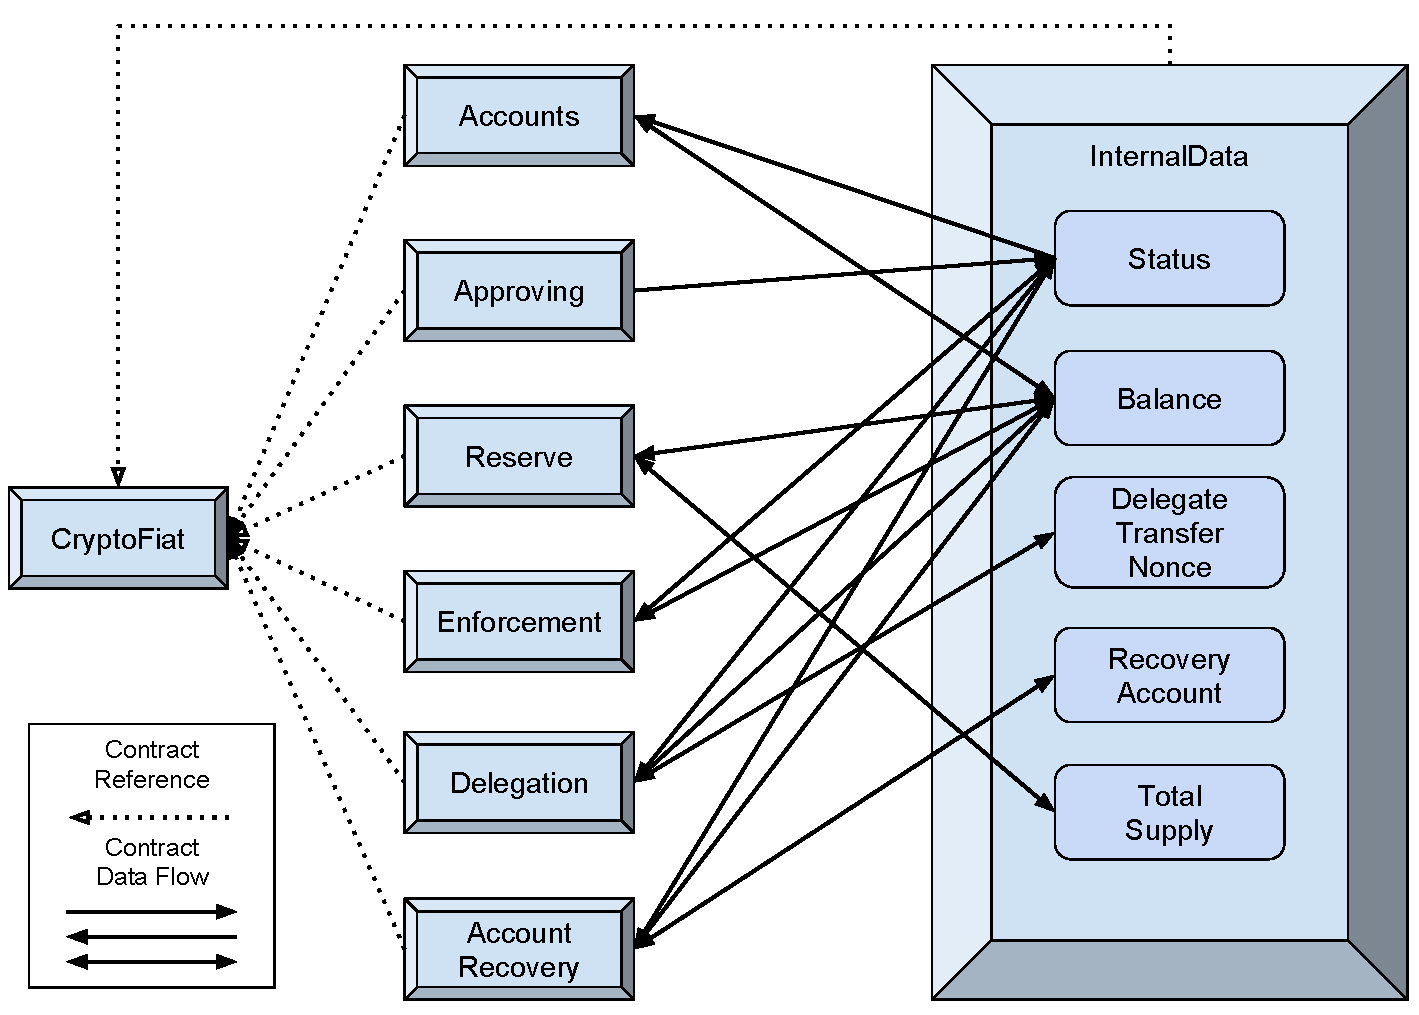
\includegraphics[width=\textwidth]{contract-data}
    \caption{Contract Data Dependencies}
    \label{fig:contractData}
\end{figure}

\begin{center}
\resizebox{\textwidth}{!}{
\begin{tabular}{ | l | l | p{12cm} | }
 \hline
 Function & Args & Description
 \\ \hline\hline
 \code{canSend} & \code{address account} & Validates if \code{account} can send by throwing an exception if it is not approved, frozen, or the address 0.
 \\ \hline
 \code{assertSend} & \code{address account} & Function form of \code{canSend}.
 \\ \hline
 \code{canReceive} & \code{address account} & Validates if \code{account} can receive by throwing an exception if it is closed or the address 0.
 \\ \hline
 \code{assertReceive} & \code{address account} & Function form of \code{canReceive}.
 \\ \hline
\end{tabular}}
\end{center}
\captionof{table}{InternalData modifiers}
\label{tab:internalDataModifiers}

\begin{center}
\resizebox{\textwidth}{!}{
\begin{tabular}{ | l | l | p{12cm} | }
 \hline
 Function & Args & Description
 \\ \hline\hline
 \code{\_withdraw} & \specialcell{\code{address account},\\ \code{uint256 amount}} & Withdraws \code{amount} from balance of \code{account}. Throws exception if \code{amount} is more than balance.
 \\ \hline
 \code{\_deposit} & \specialcell{\code{address account},\\ \code{uint256 amount}} & Deposits \code{amount} into balance for \code{account}. Throws exception if amount to withdraw plus balance is less than balance (overflow).
 \\ \hline
\end{tabular}}
\end{center}
\captionof{table}{InternalData account functions}
\label{tab:internalDataAccountFunctions}

\subsubsection{Accounts Contract} \label{sssec:3.5:accounts}
The \textit{Accounts} contract exposes all the functions, listed in \hypertableref{tab:accountsFunctions}, necessary from \textit{InternalData} to work with accounts and balances.

\begin{center}
\resizebox{\textwidth}{!}{
\begin{tabular}{ | l | l | p{12cm} | }
 \hline
 Function & Args & Description
 \\ \hline\hline
 \code{balanceOf} & \code{address account} & Returns \code{uint256} balance of \code{account}.
 \\ \hline
 \code{statusOf} & \code{address account} & Returns \code{uint256} of boolean flags with the status of \code{account} as defined in table \hypertableref{tab:constantAccountStates}.
 \\ \hline
 \code{isApproved} & \code{address account} & Returns \code{bool} whether \code{account} is approved (can send funds).
 \\ \hline
 \code{isClosed} & \code{address account} & Returns \code{bool} whether \code{account} is closed (can not receive funds).
 \\ \hline
 \code{isFrozen} & \code{address account} &  Returns \code{bool} whether \code{account} is frozen (can not send funds).
 \\ \hline
 \code{transfer} & \specialcell{\code{address destination},\\ \code{uint256 amount}} & Withdraws \code{amount} from caller \code{msg.sender} and deposits \code{amount} into \code{destination}. Restricted to \code{msg.sender} that \code{canSend} and \code{destination} that \code{canReceive}. Logs \code{Transfer} event for \code{source}, \code{destination}, and \code{amount}.
 \\ \hline
\end{tabular}}
\end{center}
\captionof{table}{Accounts functions}
\label{tab:accountsFunctions}

\subsubsection{Approving Contract} \label{sssec:3.5:approving}
\textit{Approving} contract exposes the functions necessary for approving accounts to transact in Euro 2.0. Only the \code{accountApprover}, \hypertableref{tab:approvingData}, can approve accounts. Modifiers, \hypertableref{tab:approvingModifiers} restrict access to functions, \hypertableref{tab:approvingFunctions}, to \code{accountApprover}.

\begin{center}
\resizebox{\textwidth}{!}{
\begin{tabular}{ | l | l | p{9cm} | }
 \hline
 Name & Type & Description
 \\ \hline\hline
 \code{accountApprover} & \code{address} & Account approver address.
 \\ \hline
\end{tabular}}
\end{center}
\captionof{table}{Approving contract data}
\label{tab:approvingData}

\begin{center}
\resizebox{\textwidth}{!}{
\begin{tabular}{ | l | l | p{12cm} | }
 \hline
 Function & Args & Description
 \\ \hline\hline
 \code{onlyAccountApprover} & & Validates if \code{msg.sender} is \code{accountApprover} otherwise throws an exception.
 \\ \hline
\end{tabular}}
\end{center}
\captionof{table}{Approving contract modifiers}
\label{tab:approvingModifiers}

\begin{center}
\resizebox{\textwidth}{!}{
\begin{tabular}{ | l | l | p{12cm} | }
 \hline
 Function & Args & Description
 \\ \hline\hline
 \code{appointAccountApprover} & \code{address next} & Assigns address of \code{accountApprover} to \code{next}, removing approving privileges to the old address. Restricted to \code{onlyAccountApprover}.
 \\ \hline
 \code{approveAccount} & \code{address account} & Sets status of \code{account} to APPROVED to be able to send money. Restricted to \code{onlyAccountApprover}. Logs \code{AccountApproved} event for the approved \code{account}.
 \\ \hline
 \code{approveAccounts} & \code{address[] accounts} & Sets status of each account in \code{accounts} to APPROVED to be able to send money. Restricted to \code{onlyAccountApprover}. Logs \code{AccountApproved} event for the approved \code{account}.
 \\ \hline
 \code{closeAccount} & \code{address account} & Sets status of \code{account} to CLOSED to prevent the account from receiving money. Restricted to \code{onlyAccountApprover}. Logs \code{AccountClosed} event for the closed \code{account}.
 \\ \hline
\end{tabular}}
\end{center}
\captionof{table}{Approving contract functions}
\label{tab:approvingFunctions}

\subsubsection{Reserve Contract} \label{sssec:3.5:reserve}

The \textit{Reserve} contract exposes the functions to increase and decrease supply of EUR2 in the Euro 2.0. Only the \code{reserveBank} account, \hypertableref{tab:reserveData}, can perform these tasks. The modifier in \hypertableref{tab:reserveModifiers} restrict access to functions listed in \hypertableref{tab:reserveFunctions} to \code{reserveBank}.

\begin{center}
\resizebox{\textwidth}{!}{
\begin{tabular}{ | l | l | p{9cm} | }
 \hline
 Name & Type & Description
 \\ \hline\hline
 \code{reserveBank} & \code{address} & Reserve bank address.
 \\ \hline
\end{tabular}}
\end{center}
\captionof{table}{Reserve contract data}
\label{tab:reserveData}

\begin{center}
\resizebox{\textwidth}{!}{
\begin{tabular}{ | l | l | p{12cm} | }
 \hline
 Function & Args & Description
 \\ \hline\hline
 \code{onlyReserveBank} & & Validates if \code{msg.sender} is \code{reserveBank} otherwise throws an exception.
 \\ \hline
\end{tabular}}
\end{center}
\captionof{table}{Reserve contract modifiers}
\label{tab:reserveModifiers}

\begin{center}
\resizebox{\textwidth}{!}{
\begin{tabular}{ | l | l | p{12cm} | }
 \hline
 Function & Args & Description
 \\ \hline\hline
 \code{appointReserveBank} & \code{address next} & Assigns address of \code{reserveBank} to \code{next}, removing  privileges of the old address. Restricted to \code{onlyReserveBank}.
 \\ \hline
 \code{totalSupply} & & Returns \code{uint256} total supply of Euro 2.0 system. No restrictions on calling this method.
 \\ \hline
 \code{increaseSupply} & \code{uint256 amount} & Increases supply by \code{amount} and deposits \code{amount} of newly created EUR2 to the \code{reserveBank}. Restricted to \code{onlyReserveBank} and \code{reserveBank} \code{canReceive}. Throws exception if supply plus amount overflows.
 \\ \hline
 \code{decreaseSupply} & \code{uint256 amount} & Decreases supply by \code{amount} and withdraws \code{amount} from \code{reserveBank}, destroying the EUR2. Restricted to \code{onlyReserveBank} and \code{reserveBank} \code{canSend}. Throws exception if supply is less than amount. Logs \code{SupplyChanged} for the new supply \code{amount}.
 \\ \hline
\end{tabular}}
\end{center}
\captionof{table}{Reserve contract functions}
\label{tab:reserveFunctions}

\subsubsection{Enforcement Contract} \label{sssec:3.5:enforcement}

The \textit{Enforcement} contract exposes the functions for law enforcement to freeze and seize funds. The two roles are the law enforcer, who can do the actions to freeze and seize funds, and account designator, who can control the account where the funds can be seized, described in \hypertableref{tab:enforcementData}. Modifiers in \hypertableref{tab:enforcementModifiers} restrict access to functions based on roll. The functions are listed in \hypertableref{tab:enforcementFunctions}.

\begin{center}
\resizebox{\textwidth}{!}{
\begin{tabular}{ | l | l | p{9cm} | }
 \hline
 Name & Type & Description
 \\ \hline\hline
 \code{lawEnforcer} & \code{address} & Law enforcer address.
 \\ \hline
 \code{accountDesignator} & \code{address} & Account designator address.
 \\ \hline
 \code{account} & \code{address} & Law enforcement account.
 \\ \hline
\end{tabular}}
\end{center}
\captionof{table}{Enforcement contract data}
\label{tab:enforcementData}

\begin{center}
\resizebox{\textwidth}{!}{
\begin{tabular}{ | l | l | p{12cm} | }
 \hline
 Function & Args & Description
 \\ \hline\hline
 \code{onlyLawEnforcer} & & Validates if \code{msg.sender} is \code{lawEnforcer} otherwise throws an exception.
 \\ \hline
 \code{onlyAccountDesignator} & & Validates if \code{msg.sender} is \code{accountDesignator} otherwise throws an exception.
 \\ \hline
\end{tabular}}
\end{center}
\captionof{table}{Enforcement contract modifiers}
\label{tab:enforcementModifiers}

\begin{center}
\resizebox{\textwidth}{!}{
\begin{tabular}{ | l | l | p{12cm} | }
 \hline
 Function & Args & Description
 \\ \hline\hline
 \code{appointLawEnforcer} & \code{address next} & Assigns address of \code{lawEnforcer} to \code{next}, removing privileges of the old address. Restricted to \code{onlyLawEnforcer}.
 \\ \hline
 \code{appointAccountDesignator} & \code{address next} & Assigns address of \code{accountDesignator} to \code{next}, removing privileges of the old address. Restricted to \code{onlyAccountDesignator}.
 \\ \hline
 \code{withdraw} & \specialcell{\code{address from}, \\ \code{uint256 amount}} & Withdraws \code{amount} from account \code{from} and deposits \code{amount} into law enforcement \code{account}. Restricted to \code{onlyLawEnforcer} and \code{account} \code{canReceive}. Logs \code{Transfer} event with \code{from}, designator \code{account}, and \code{amount}.
 \\ \hline
 \code{freezeAccount} & \code{address target} & Sets status of \code{target} account to FROZEN so it can no longer send funds. Restricted to \code{onlyLawEnforcer}. Logs \code{AccountFreeze} event with \code{target} and value {true}.
 \\ \hline
 \code{unFreezeAccount} & \code{address target} & Removes FROZEN status of \code{target} account so it can send funds again. Restricted to \code{onlyLawEnforcer}. Logs \code{AccountFreeze} event with \code{target} and value \code{false}.
 \\ \hline
 \code{designateAccount} & \code{address account} & Sets law enforcement \code{account} to given \code{account}. Restricted to \code{onlyAccountDesignator} and \code{account} \code{canReceive}.
 \\ \hline
\end{tabular}}
\end{center}
\captionof{table}{Enforcement contract functions}
\label{tab:enforcementFunctions}

\subsubsection{AccountRecovery Contract} \label{sssec:3.5:accountRecovery}

The \textit{AccountRecovery} exposes functionality intended for an account recovery mechanism. An account owner can designate a trusted party to withdraw all funds and close the account. The two functions enabling this functionality are listed in \hypertableref{tab:accountRecoveryFunctions}.

\begin{center}
\resizebox{\textwidth}{!}{
\begin{tabular}{ | l | l | p{12cm} | }
 \hline
 Function & Args & Description
 \\ \hline\hline
 \code{designateRecoveryAccount} & \code{address recoveryAccount} & Sets the recovery account for \code{msg.sender} to address \code{recoveryAccount}, replacing an existing \code{recoveryAccount}. To remove a recovery account the address 0 can be set.
 \\ \hline
 \code{recoverBalance} & \specialcell{\code{address from}, \\ \code{address into}} & Withdraws all funds from account \code{from} and deposits all funds to account \code{into} and then closing account \code{from} by setting its status to CLOSED. Restricted to account \code{from} \code{canSend} and account \code{into} \code{canReceive}. Logs \code{AccountClosed} event of \code{from} account and \code{Transfer} event of \code{from} account, \code{into} account, and \code{amount}.
 \\ \hline
\end{tabular}}
\end{center}
\captionof{table}{AccountRecovery contract functions}
\label{tab:accountRecoveryFunctions}

\subsubsection{Delegation Contract} \label{sssec:3.5:delegation}

\todo[inline]{The \textit{Delegation} contract is magic...}
Its functions are listed in \hypertableref{tab:delegationFunctions}}.

\begin{center}
\resizebox{\textwidth}{!}{
\begin{tabular}{ | l | l | p{12cm} | }
 \hline
 Function & Args & Description
 \\ \hline\hline
 \code{nonceOf} & \code{address account} & Sets delegated transfer nonce of \code{account}.
 \\ \hline
 \code{transfer}
    & \specialcell{
 		% transfer request
        \code{uint256 nonce}, \\
		\code{address destination}, \\
		\code{uint256 amount}, \\
		\code{uint256 fee}, \\
        % transfer request signed by source
        \code{bytes signature}, \\
        % whom to pay for fulfilling transfer
        \code{address delegate}
 	   }
    & Makes a delegate transfer from a \code{source} account, recovered by extracting public key from elliptic curve \code{signature}, to \code{destination} of \code{amount} with fee \code{fee} paid to \code{delegate}. \code{nonce} is used to prevent replay attacks. Logs \code{Transfer} event for \code{source} account (in signature), \code{destination}, and \code{amount} and if there is a fee, also logs \code{Transfer} event for \code{source}, \code{delegate}, and the \code{fee}.
 \\ \hline
 \code{multitransfer}
 	& \specialcell{\code{uint256 count}, \\ \code{bytes transfers}, \\ \code{address delegate}}
	& Performs the same logic as \code{transfer} for \code{count} number of transfers encoded in \code{transfers} byte array.
 \\ \hline
\end{tabular}}
\end{center}
\captionof{table}{Delegation contract functions}
\label{tab:delegationFunctions}

\subsection{Centralized Components} \label{ssec:3.5}

The centralized components of the Euro 2.0 prototype are built with traditional client server architecture. Currently these are maintained by the Euro 2.0 Foundation, but would ideally be given over to government or the central bank to run their own monetary system. We only give a high level overview of the centralized component architecture, not going into any significant details of their implementation. At the time of the writing the components are based off of an unfinished prototype with quite a few bugs and some components not yet built. The goal of the subsection is to describe how the centralize components could be set up in such a system, where are the important keys and data are held, and in \hypersectionref{ssec:3.6} how these components interact with the client and Ethereum to fulfill the features described in \hypersectionref{ssec:3.2}.

\hyperfigureref{fig:euro2architecture} shows the architecture of the Euro 2.0 digital currency showing the interaction between both centralized and decentralized components. The figure is quite a helpful reference point when relating the components to their place in the system.

\begin{figure}[ht]
    \centering
    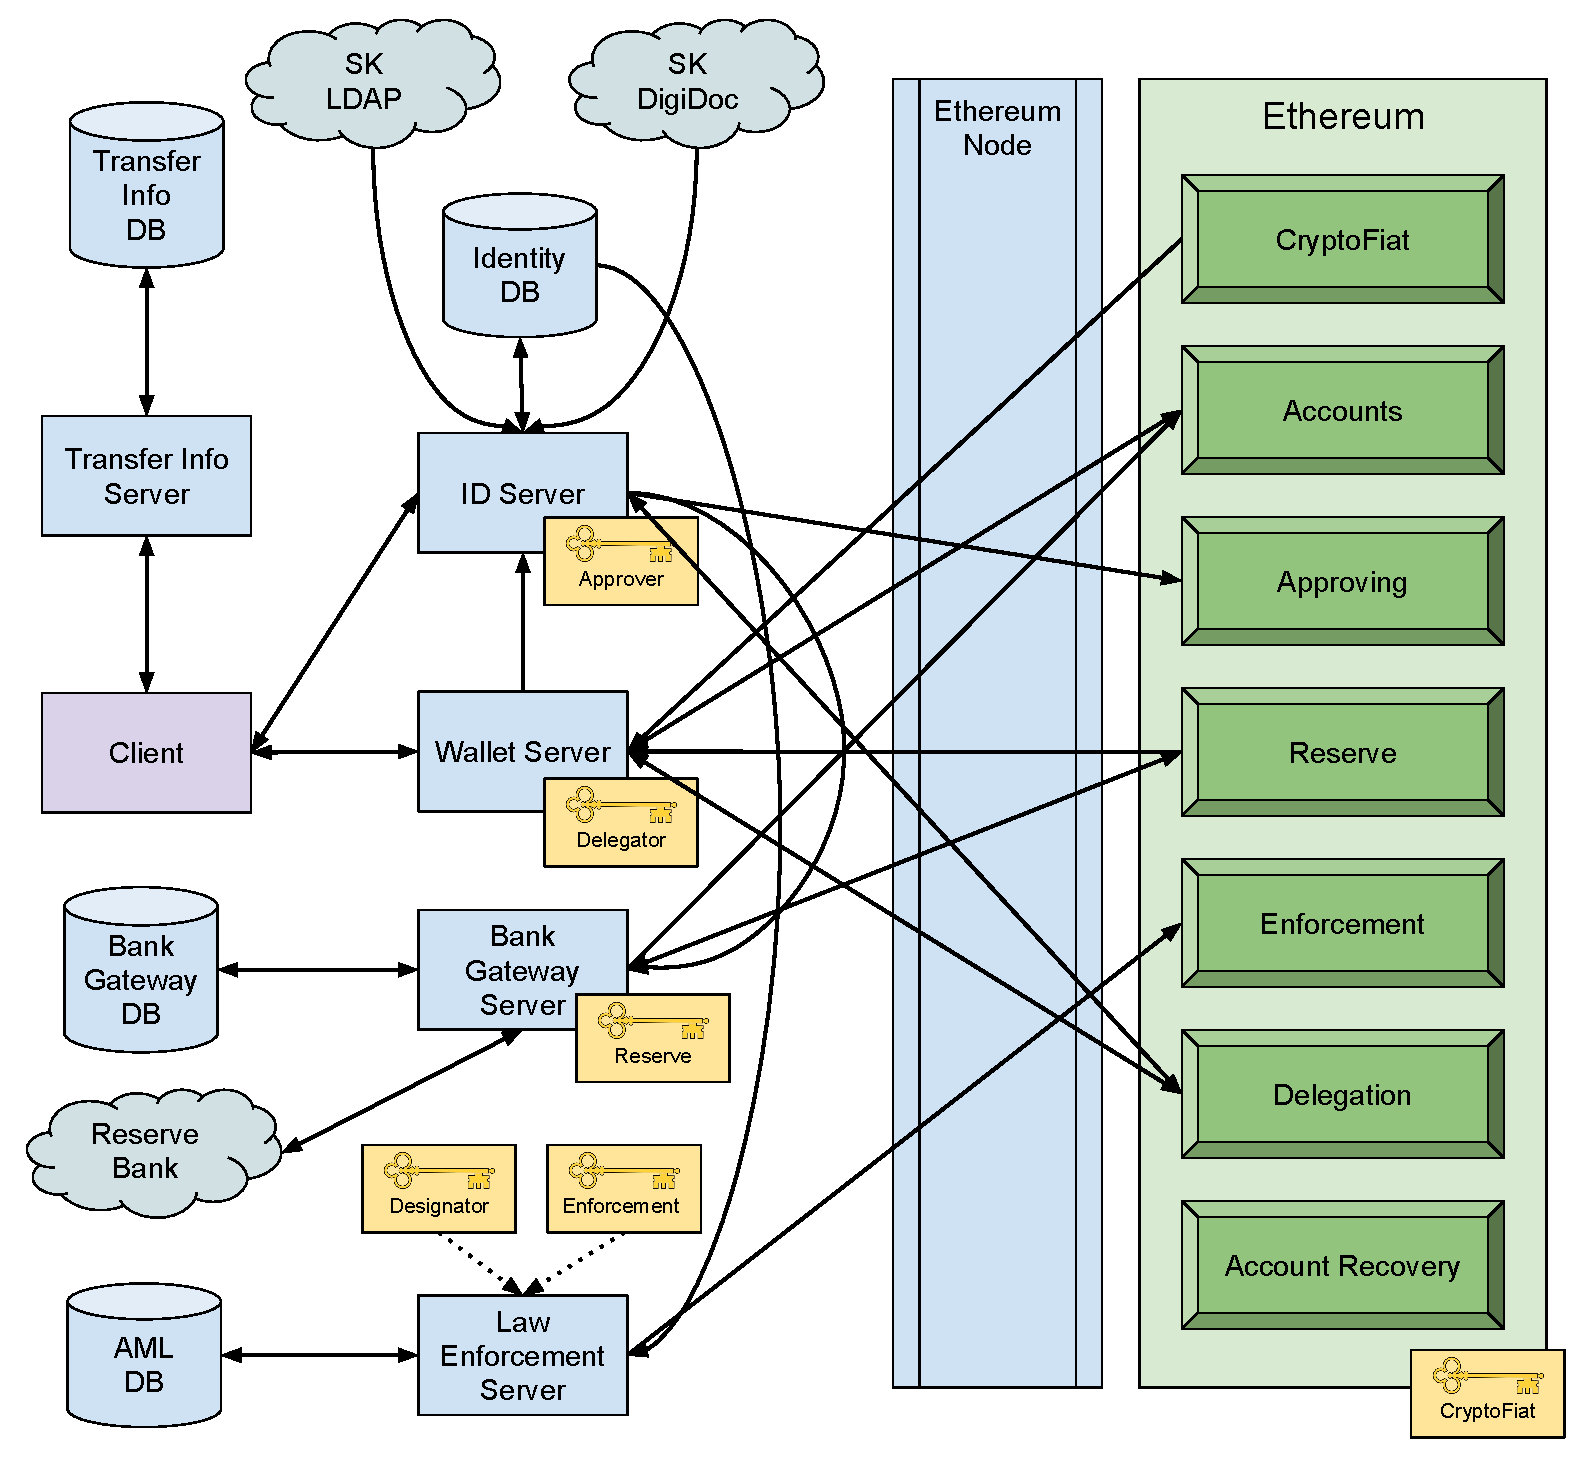
\includegraphics[width=\textwidth]{euro2-architecture}
    \caption{Euro 2.0 Architecture}
    \label{fig:euro2architecture}
\end{figure}

\subsubsection{Client} \label{sssec:3.5:client}
For our purposes the client refers to code running on a user's device interacting with the Euro 2.0 system. This can be a smart phone application or laptop browser. This is typically Javascript displaying the UI and making HTTP REST calls to the servers for interactions with the system. In the current prototype the client library does not interact directly with the decentralized components, but goes through the servers for all actions. The client will typically be storing a user's private keys in order to access their EUR2 funds.

\subsubsection{ID Server} \label{sssec:3.5:idServer}
The ID server is an interface to all the ID operations of the system. It's main functions include:

\begin{itemize}
	\item Authorization process for ID card, mobile ID, or bank transfer
	\item Approving addresses authorized by an ID
	\item Maintaining the mapping between addresses and ID
	\item Create and Claim Escrowed funds to an ID
	\item Addresses and keys backup system for an ID
\end{itemize}

\subsubsection{ID Database} \label{sssec:3.5:idDatabase}

The ID Database holds the data needed for the ID server. The tables include:

\begin{center}
\begin{tabular}{ | l | p{10cm} | }
 \hline
 \textbf{backup\_challenge} & ...
 \\ \hline\hline
 id\_code & ...
 \\ \hline
 plaintext & ...
 \\ \hline
 encrypted & ...
 \\ \hline
 active & ...
 \\ \hline
\end{tabular}
\end{center}
\captionof{table}{Id Database Backup Challenge Table}
\label{tab:idDatabaseBackupChallenge}

\begin{center}
\begin{tabular}{ | l | p{10cm} | }
 \hline
 \textbf{escrow} & ...
 \\ \hline\hline
 id\_code & ...
 \\ \hline
 private\_key & ...
 \\ \hline
 address & ...
 \\ \hline
 cleared & ...
 \\ \hline
 clearing\_hash & ...
 \\ \hline
\end{tabular}
\end{center}
\captionof{table}{ID Database Escrow Table}
\label{tab:idDatabaseEscrow}

\begin{center}
\begin{tabular}{ | l | p{10cm} | }
 \hline
 \textbf{ethereum\_account} & ...
 \\ \hline\hline
 owner\_id & ...
 \\ \hline
 address & ...
 \\ \hline
 activated & ...
 \\ \hline
 creation\_time & ...
 \\ \hline
 modification\_time & ...
 \\ \hline
 authorisation\_type & ...
 \\ \hline
 transaction\_hash & ...
 \\ \hline
\end{tabular}
\end{center}
\captionof{table}{ID Database Ethereum Address Table}
\label{tab:idDatabaseEthereumAddress}

\begin{center}
\begin{tabular}{ | l | p{10cm} | }
 \hline
 \textbf{ethereum\_account} & ...
 \\ \hline\hline
 key\_backup & ...
 \\ \hline
 challenge & ...
 \\ \hline
 address & ...
 \\ \hline
 key\_enc & ...
 \\ \hline
 active & ...
 \\ \hline
\end{tabular}
\end{center}
\captionof{table}{ID Database Key Backup Table}
\label{tab:idDatabaseKeyBackup}

\begin{center}
\begin{tabular}{ | l | p{10cm} | }
 \hline
 \textbf{ethereum\_account} & ...
 \\ \hline\hline
 ldap\_response & ...
 \\ \hline
 id\_code & ...
 \\ \hline
 first\_name & ...
 \\ \hline
 last\_name & ...
 \\ \hline
\end{tabular}
\end{center}
\captionof{table}{ID Database LDAP Response Table}
\label{tab:idDatabaseLdapResponse}

\begin{center}
\begin{tabular}{ | l | p{10cm} | }
 \hline
 \textbf{pending\_authorisation} & ...
 \\ \hline\hline
 auth\_identifier & ...
 \\ \hline
 type & ...
 \\ \hline
 address & ...
 \\ \hline
 serialised\_mobile\_id\_session & ...
 \\ \hline
 creation\_time & ...
 \\ \hline
 modification\_time & ...
 \\ \hline
 bank\_transfer\_payment\_reference & ...
 \\ \hline
\end{tabular}
\end{center}
\captionof{table}{ID Database Pending Authorization Table}
\label{tab:idDatabasePendingAuthorization}

\subsubsection{SK LDAP Directory Service}

Estonian certificate center (SK)\cite{aboutSk2017} provides an LDAP (Lightweight Directory Access Protocol) server to look up public certificates and legal name for a given Estonia ID number\cite{skAboutLdap2017}\cite{skLdapTechnical2017}. This service is the provider for ID server to look up real names given an Estonian ID code.

\subsubsection{SK DigiDocService}

Estonian certificate center (SK) provides a DigiDocService which allows registered services to provide the ability for users to authenticate themselves with Estonian Mobile-ID or ID card\cite{skDigiDocService2017}. This service is the provider for ID Server to authenticate users using their Mobile ID or Estonian ID card.

\subsubsection{Wallet Server} \label{sssec:3.5:walletServer}

Wallet server is the main entry point for conveniently creating transactions in the Euro 2.0 system and retrieving data from Etherum. It provides the following functionality:

\begin{itemize}
	\item Get transaction info for a transaction hash
	\item Create delegated transfer to another an approved address where the server pays the ether
	\item Create transfer to a bank account via a delegated transfer to the reserve bank
	\item Get address status, balance, and delegate transfer nonce
	\item Get all transfers involving an address
	\item Get transfer fees in EUR2
	\item Get supply amount
\end{itemize}

\subsubsection{Transfer Details Server} \label{sssec:3.5:transferDetailsServer}

Transfer info server has a single purpose of saving transfer info for transactions off chain. It provides a general purpose interface that is up to the client to ensure proper encryption of transfer details so that sender and recipient can view the details. The functionality is simply:

\begin{itemize}
	\item Save transfer details for a transaction hash
	\item Load transfer details for a transaction hash
\end{itemize}

\subsubsection{Transfer Info Database} \label{sssec:3.5:transferInfoDatabase}

This is the database providing for the Transfer Info Server. It's simply a key value store with transaction hash as the key and a blob of data as the value (reference implementation is Google's LevelDB).

\subsubsection{Bank Gateway} \label{sssec:3.5:bankGateway}

The Bank Gateway is the entry point for the real euros in Euro 2.0. The functionality includes:

\begin{itemize}
	\item Update total reserve from uploaded bank statement files
	\item Update total supply
	\item Parse received EUR transactions and send EUR2 to addresses
	\item Handle EUR2 to EUR payments
\end{itemize}

\subsubsection{AML Server} \label{sssec:3.5:amlServer}

The AML server provides the functionality to law enforcement to police the system, including:

\begin{itemize}
	\item Convenience interface for freezing and seizing funds
	\item Convenience interface for accessing AML database
	\item Runs jobs to fill AML database with transaction data
	\item Runs name check jobs on user identities
\end{itemize}

\subsubsection{AML Database} \label{sssec:3.5:amlDatabase}

The AML database provides law enforcement the transaction and identity data needed for AML investigations.

\subsubsection{Ethereum Gateway} \label{sssec:3.5:ethereumGateway}

The Ethereum Gateway is an ethereum full node able to process Ethereum JSON-RPC calls to post and receive data from the Ethereum network. All RPC calls from centralized components go through this interface.

\subsection{Fulfillment of Features} \label{ssec:3.6}

\todo[inline]{Write how the features are fulfilled (with many many diagrams)}

\subsection{Conclusion} \label{ssec:3.7}

\todo[inline]{Write Chapter 3 conclusion}

\pagebreak

%--------------------CHAPTER 4-----------------
\section{Chapter 4} \label{sec:4}

\subsection{Introduction} \label{ssec:4.1}

In this chapter we explore the social technical implications of the Euro 2.0 system on key stakeholders. We do this by exploring the research question:

\begin{quoting}
	\textbf{RQ2:} \textit{How does adoption of Euro 2.0 digital currency impact the relationship with money for key stakeholders: users, merchants, governments, and banks?}
\end{quoting}

In which we explore in the following sub research questions.

\begin{quoting}
	\textbf{RQ2.1:} \textit{What is the current relationship of money for stakeholders?}
\end{quoting}
\begin{quoting}
	\textbf{RQ2.2:} \textit{What changes in the relationship of money for stakeholders after adopting the Euro 2.0 digital currency?}
\end{quoting}
\begin{quoting}
	\textbf{RQ2.3:} \textit{What are the enabling and inhibiting factors influencing the transition to the Euro 2.0 digital currency?}
\end{quoting}

We approach the research questions design and UX influenced interpretation of the \textit{Change Formula} from the field of Organization Development\cite{dannemiller1992}. In \hypersectionref{ssec:4.2} we define methods and terminology of the analysis, first the \textit{Change Formula}, then our interpretation \textit{Change Analysis}, and then define the stakeholders of Euro 2.0 system for the analysis. In \hypersectionref{ssec:4.3} we answer \textbf{RQ2.1} by describing the current state of money for each stakeholder. Likewise in \hypersectionref{ssec:4.4} we answer \textbf{RQ2.2} by describing the future state of money for each stakeholder under hypothetical use of the Euro 2.0 digital currency. Note in both \ref{ssec:4.3} and \ref{ssec:4.4} we use state and relationship interchangeably to correspond to \textit{Change Analysis} terminology. In \hypersectionref{ssec:4.5} we perform the change analysis for each stakeholder to answer \textbf{RQ2.3} describing potential enablers and inhibitors to change to a digital currency system. And finally we summarize our findings and future work in the conclusion, \hypersectionref{ssec:4.6}.

\subsection{Analysis Preparation} \label{ssec:4.2}

\subsubsection{Change Formula} \label{sssec:4.2:changeFormula}
The \textit{Change Formula} was originally written on a chalkboard by scientist David Gleicher and stuck in the mind of organizational behavior expert Richard Beckhard\cite{changeFormula2014}. The formula was first published in Sloan Management Review\cite{beckhard1975} and later in book by Beckhard and Harris\cite{organizationalTransitions1977}. Succinctly described in the review paper, Cady et al., \textit{``The formula describes the conditions, that when met, will move an individual, group, or whole system in a direction of their choosing.''} \cite{changeFormula2014}.

The improved version of the formula by Dannemiller\cite{dannemiller1992} states that change will occur when the following condition is satisfied:

\begin{equation}
	D \times V \times F > R
\end{equation}

\begin{itemize}
	\item $D$ : Dissatisfaction with the present situation
	\item $V$ : Vision of what is possible
	\item $F$ : First steps towards reaching the vision
	\item $R$ : Resistance to change
\end{itemize}

If any one of $D$, $V$, or $F$ is zero, i.e. neglected or overlooked, then the resistance to change will not be overcome and the intended behavioral change will not ensue.

We use the \textit{Change Formula} in the context of Euro 2.0 to analyze the change of stakeholders using Euro 2.0 digital currency instead of Euro in the traditional monetary system. This is the academic basis of the analysis technique proposed in the following section.

\subsubsection{Change Analysis} \label{sssec:4.2:changeAnalysis}

\textit{Change Analysis} is a UX and User Design interpretation of the \textit{Change Formula}. It is a framework to analyze how a new system will affect key stakeholders and seeds future design research. The concepts of \textit{Change Analysis} are depicted in \hyperfigureref{fig:changeAnalysis} and described below. Stakeholders refer to human or organizational actors interacting with the system.

\textbf{Current State} is the current state of the world for the stakeholders before the proposed change. This includes actions and functions stakeholders can do, motivations and psychological factors, as well as consequences and side-affects of these functions. In regards to the Change Formula, the current state includes the dissatisfaction $D$ and provides a starting point for listing factors influencing first steps $F$ and resistance $R$.

\textbf{Future State} is the state of the world after the proposed change. This also includes actions and functions stakeholders can do, motivations and psychological factors, as well as consequences and side-affects of these functions. In regards to the Change Formula, the future state is the vision of change $V$.

\textbf{Enablers} are the \textit{Patterns}, \textit{Habits}, \textit{Behaviors}, and \textit{Motivation} in the current state that would indicate stakeholders are ready to adapt proposed change in the future state of the world. In regards to the Change Formula, enablers are those factors supporting first steps to the change $F$.

\textbf{Inhibitors} are the factors in the current state that would discourage stakeholders from the proposed change to the future state of world including \textit{Existing Policy Legislation}, \textit{Parties with Vested Interest}, \textit{Infrastructure and Technology}, and \textit{Personal Barriers to Change}. In regards to the Change Formula, inhibitors are those factors contributing to resistance of change $R$.

The outcome of the change analysis is an understanding of how the change will impact the stakeholders, a set of inhibitors and enablers for that change, and further areas of design research to validate or disprove the hypotheses.

\begin{figure}[ht]
    \centering
    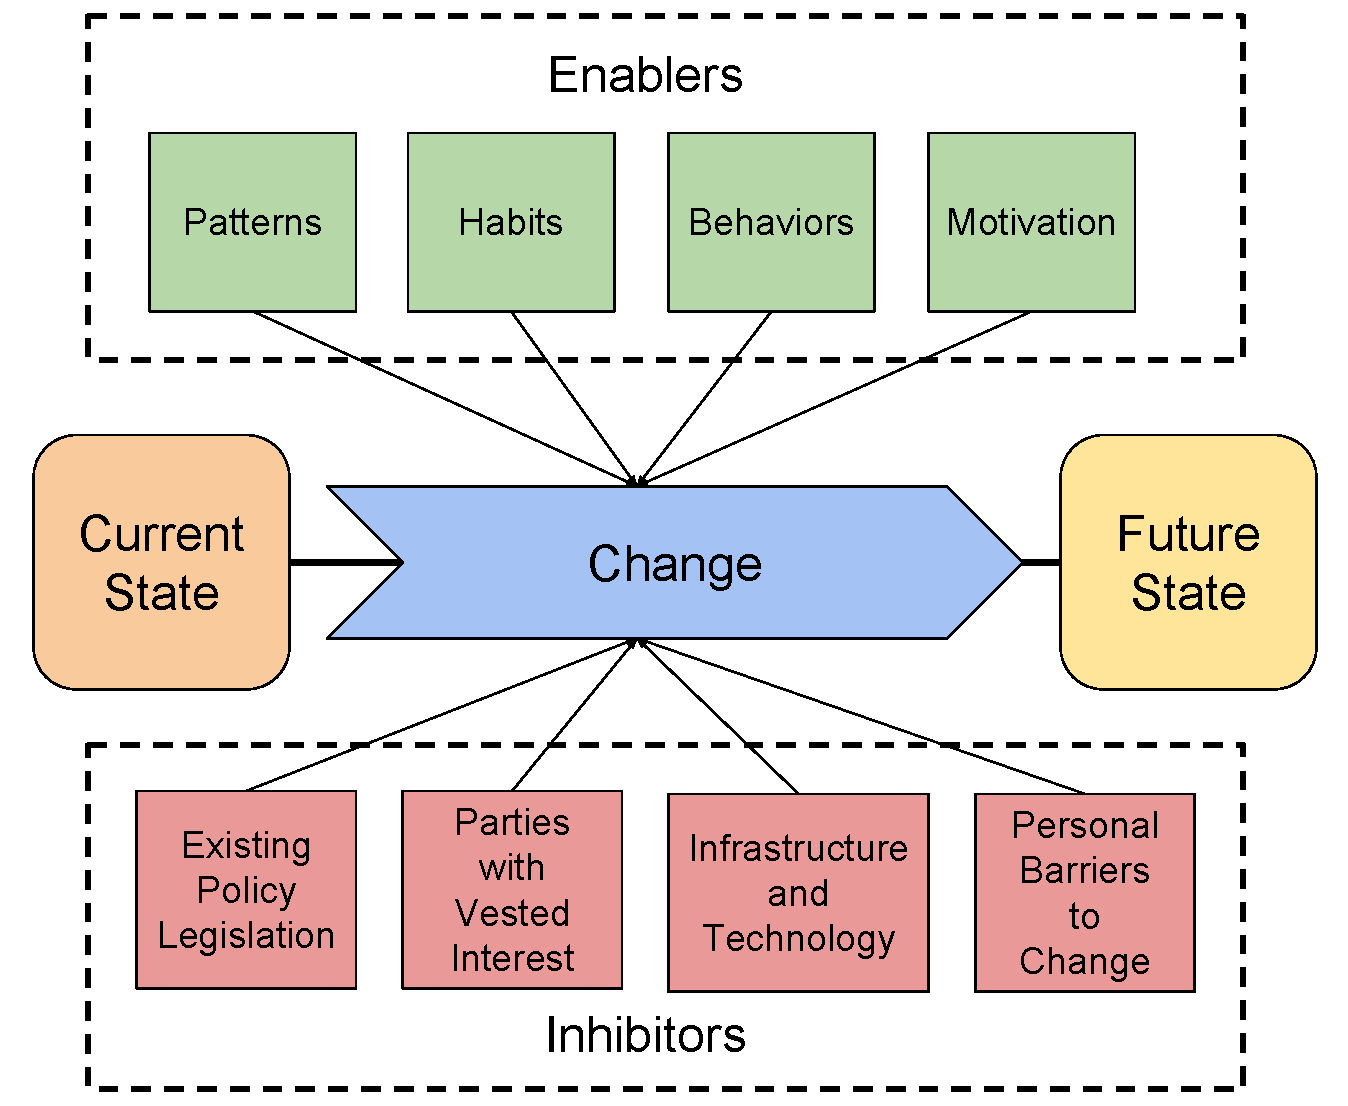
\includegraphics[width=\textwidth]{change-analysis}
    \caption{Change Analysis Overview}
    \label{fig:changeAnalysis}
\end{figure}

\subsubsection{Key Stakeholders} \label{sssec:4.2:keyStakeholders}

The key stakeholders of the Euro 2.0 system are listed below.

\textbf{Users} are everyday users of financial systems sending and receiving transactions for personal use.

\textbf{Merchants} represent businesses users of financial system sending and receiving money for business use. In the context of this analysis we use merchants as the first use case representative of business entities.

\textbf{Banks} represent financial institutions in the financial system, including traditional banks and payment processors. For this analysis a bank is both a traditional bank making money off of holdings and a payment processor making money off of transactions.

\textbf{Government} represents the government entities in a financial system including the regulators defining the rules of a financial system, the central bank managing the economic value of the fiat currency, the law enforcement policing money, and the tax board collecting taxes.

\subsection{Current State of Money} \label{ssec:4.3}

In this section we describe the \textit{Current State} of money for each stakeholder.

\subsubsection{Current State: Users} \label{sssec:4.3:users}

Users of the current monetary system have the following functions and use cases:

\begin{itemize}
	\item Use bank transfers to make payments
	\item Use credit and debit cards to make payments
	\item Use bank accounts for short term and long term storage of funds
	\item Use cash for off record transactions
	\item Exchange money for goods and services
	\item Pay bills
	\item Settle small debts
	\item Save money
	\item Invest and grow money
	\item Borrow money
	\item Keep account numbers and access credentials secure
\end{itemize}

Users are influenced by the following psychological factors and behaviors:

\begin{itemize}
	\item They want to keep their money
	\item They don't trust themselves with a significant amount of money
	\item They don't trust others with their money
	\item They believe in rules and repercussions of breaking the rules
	\item They like to outsource functions to experts
	\item They do what other people do
	\item They deal only with very small fragments of financial institutions
\end{itemize}

The current side affects and consequences of the monetary system for users are:

\begin{itemize}
	\item They make money by working
	\item They make money by investing
	\item They lose money in transaction fees
	\item They lose money in financial crime
	\item They lose money in bad investments
	\item They lose money by spending
	\item They lose money by inflation
	\item They lose money by currency exchange rate movements
\end{itemize}

\subsubsection{Current State: Merchants} \label{sssec:4.3:merchants}

Merchants in the current monetary system have the following functions and use cases:

\begin{itemize}
	\item They accept payments for goods and services
	\item They accept cash payments
	\item They accept online payments
	\item They accept card payments
	\item They accept bank transfers
	\item They pay employees
	\item They invest money in the business
	\item They track money (accounting)
	\item They borrow money for the business
\end{itemize}

Merchants are influenced by the following psychological factors and behaviors:

\begin{itemize}
	\item They need to cater to convenience of customers
	\item They want to make money
	\item They want to be ahead of their competitors
	\item They want to stay in business
\end{itemize}

The current side affects and consequences of the monetary system for merchants are:

\begin{itemize}
	\item They make money from profit
	\item They lose money to reversible payments
	\item They lose money to transaction fees
	\item They lose money from money admin fees
	\item They lose money to opportunity cost of stuck money
	\item They lose money by spending
	\item They lose money from inflation
	\item They lose money from currency fluctuations
\end{itemize}

\subsubsection{Current State: Banks} \label{sssec:4.3:banks}

Banks in the current monetary system have the following functions and use cases:

\begin{itemize}
	\item They keep other people's money safe
	\item They make money with other peoples' money
	\item They keep track of other peoples' money
	\item They offer money through loans
	\item They facilitate transactions
	\item They hold balances of money
	\item They offer financial instruments to protect other peoples' money
	\item They verify and identify people for KYC/AML
	\item They pay salaries of employees
\end{itemize}

Banks are influenced by the following psychological factors and behaviors:

\begin{itemize}
	\item They want to make money
	\item They want to incentivize people to give them their money
	\item They want to keep regulators happy
\end{itemize}

The current side affects and consequences of the monetary system for banks are:

\begin{itemize}
	\item They make money from transactions
	\item They make money from account admin fees
	\item They make money from interests on loans
	\item They make money through investing other peoples' money
	\item They make money on hedging and other financial instruments
	\item They lose money on miscalculated hedges and backfiring financial instruments
	\item They lose money on bad investments
	\item They lose money on defaulted loans
	\item They lose money on fines
	\item They lose money on financial crime
\end{itemize}

\subsubsection{Current State: Government} \label{sssec:4.3:government}

Government in the current monetary system has the following functions and use cases:

\begin{itemize}
	\item It collects taxes of all citizens and businesses
	\item It pays salaries of employees
	\item It buys goods and services for the state
	\item It sets the monetary policies
	\item It tracks money
	\item It freezes assets of criminals
	\item It enforces policy through audits
	\item It issues documents used to verify identities
	\item It borrows money
	\item It loans money
	\item It collects fines
	\item It pays benefits
	\item It issues currency and tracks total currency in the system
\end{itemize}

Government is influenced by the following factors:

\begin{itemize}
	\item It wants to keep the economy profitable for the country
	\item It wants to ensure the wellbeing of its citizens
	\item It wants to keep itself in power
	\item It wants to ensure the viability of its currency
\end{itemize}

The current side affects and consequences of the monetary system for government are:

\begin{itemize}
	\item Loses money in tax evasion
	\item Loses money on defaulted loans
\end{itemize}

\subsection{Future State of Money} \label{ssec:4.4}

In this subsection we look at the future state of money under adoption of Euro 2.0 system for stakeholders. In \hypersectionref{sssec:4.4:euro2} we describe the key changes of the Euro 2.0 system on the relationship with money. Then we describe what changes for the stakeholders in the following sections \hypersectionref{sssec:4.4:users}, \hypersectionref{sssec:4.4:merchants}, \hypersectionref{sssec:4.4:banks}, and \hypersectionref{sssec:4.4:government}.

\subsubsection{Future State: Euro 2.0} \label{sssec:4.4:euro2}

The key changes imposed by the Euro 2.0 system are as follows:

\begin{itemize}
	\item Transactions and balances are on a public ledger for Ethereum addresses
	\item Financial institutions are no longer needed to do transactions and store balances
	\item Publicly accessible decentralized computing network for transactions
	\item Reserve bank can convert back and forth from euro and digital euro
	\item Ability to send and receive money directly to Estonian ID codes
	\item Euros encoded as secret cryptographic keys
	\item All Ethereum addresses in the system are linked to real identities
	\item No money admin fees for holding in the system
	\item Irreversible transactions
\end{itemize}

The side effects of the euro 2.0 system:

\begin{itemize}
	\item All transactions must performed online
	\item Losing cryptographic keys loses access to funds (unless they are recovered or seized)
	\item Identifying an owner behind an Ethereum address reveals the entire balance and transaction history of that address for that owner
\end{itemize}

\subsubsection{Future State: Users} \label{sssec:4.4:users}

What changes particularly for users in the Euro 2.0 system are:

\begin{itemize}
	\item Less fees when financial intermediary is removed from transactions
	\item The good and bad side affects of transparency of money
	\item No money stuck in transit in pending transactions
	\item Money can be moved 24/7
	\item Simpler taxes
	\item Limited to transact with on record goods and services (no under the table cash transactions)
\end{itemize}

\subsubsection{Future State: Merchants} \label{sssec:4.4:merchants}

What changes particularly for merchants in the Euro 2.0 system are:

\begin{itemize}
	\item Less fees when financial intermediary is removed from transactions
	\item Every transaction automatically on record
	\item The good and bad side affects of transparency of money
	\item No money stuck in transit in pending transactions
	\item Money can be moved 24/7
	\item Simpler taxes
	\item Limited to transact with on record goods and services (no under the table cash transactions)
\end{itemize}

\subsubsection{Future State: Banks} \label{sssec:4.4:banks}

What changes particularly for banks in the Euro 2.0 system are:

\begin{itemize}
	\item No longer holding other people's money
	\item No longer collecting transaction fees
	\item Must invest in new service offerings to attract customers
	\item May run into severe lack of capital if enough people use the system
\end{itemize}

\subsubsection{Future State: Government} \label{sssec:4.4:government}

What changes particularly for government in the Euro 2.0 system are:

\begin{itemize}
	\item More easy to track money
	\item Can freeze and seize assets more easily
	\item Can collect taxes without a middleman or fees
	\item Can allow realtime tax collection
	\item Eliminate tax evasion
	\item Clear accurate statistics of the state and amount of money in the entire monetary system
\end{itemize}

\subsection{Changes Analysis} \label{ssec:4.5}

In this section we present the \textit{Inhibitors} and \textit{Enablers} of change for each stakeholder of the Euro 2.0 system.

\subsubsection{Change Analysis: Users} \label{sssec:4.5:users}

\paragraph*{Enablers}

\begin{itemize}
	\item Users are growing increasingly distrustful against banks and financial institutions after the 2008 financial crisis.
	\item Users are starting to consider and adopt Bitcoin and other cryptocurrencies for finances and investments.
	\item Users would like to reduce fees and increase the availability of their assets.
	\item Users are starting to turn more and more to cards and electronic forms of payment.
\end{itemize}

\paragraph*{Inhibitors}

\begin{itemize}
	\item Users are may not be ready to manage their own money.
	\item Users do not see how banks make money off of holding their financial assets and keep most of the return.
	\item Users are already comfortable with the existing financial system.
	\item Users will not adopt a new digital currency if the goods and services they use everyday do not accept the digital currency.
	\item Users are not ready or don't understand the implications of a public ledger of transactions.
	\item Regulations may lag to protect users from crime using digital currency.
\end{itemize}

\subsubsection{Change Analysis: Merchants} \label{sssec:4.5:merchants}

\paragraph*{Enablers}

\begin{itemize}
	\item Merchants save will save a lot of money accepting payment with low fees of digital currency over existing solutions.
	\item Merchants will save a lot of time with automation of accounting and taxes.
	\item Merchants will not have to worry about chargebacks and fraud risks of reversible payment methods.
	\item Merchants will not be affected by delays of pending payments.
\end{itemize}

\paragraph*{Inhibitors}

\begin{itemize}
	\item Merchants may not move to the new system if users are not ready to use it.
	\item Merchants dealing with cash for off record transactions have no incentive to use an on record system.
	\item Installing new technology or systems to accept payments has overhead.
	\item Accounting and tax firms will resist automation of these processes.
\end{itemize}

\subsubsection{Change Analysis: Banks} \label{sssec:4.5:banks}

\paragraph*{Enablers}

\begin{itemize}
	\item Banks show interest in using distributed ledger technology in intra bank processes.
	\item Banks want to offer convenience to their users.
	\item Banks are in the best position to offer a convenient interface for digital currency.
\end{itemize}

\paragraph*{Inhibitors}

\begin{itemize}
	\item Resistance to accepting Bitcoin as valid payment method.
	\item Resistance to incorporate new technology into their processes.
	\item No longer profit from transaction fees.
	\item No longer profit from investing other peoples' money.
	\item Unwilling to have information about financials in the public ledger.
	\item Lack of trust in a public distributed network handling finance.
\end{itemize}

\subsubsection{Change Analysis: Government} \label{sssec:4.5:government}

\paragraph*{Enablers}

\begin{itemize}
	\item Governments are becoming more interested in digital currency.
	\item Governments are starting to regulate Bitcoin and other cryptocurrency through exchanges.
	\item Governments want to see more into the flow and use of money for tax and law enforcement reasons.
\end{itemize}

\paragraph*{Inhibitors}

\begin{itemize}
	\item Banks may lobby Governments against adoption of a digital currency affecting their core business model.
	\item Government may not have the expertise or capacity to launch and maintain a digital currency like Euro 2.0.
	\item Government may not understand exactly the benefits or intricacies of a digital currency.
	\item Regulation may be too inflexible to allow for creation of a digital currency.
\end{itemize}

\subsection{Conclusion} \label{ssec:4.6}

In this chapter we presented a change analysis of the stakeholders of the Euro 2.0 system. In \hypersectionref{ssec:4.2} we presented the \textit{Change Formula} and the interpreted a \textit{Change Analysis} framework. In \hypersectionref{ssec:4.3} we presented the  current relationship of stakeholders with money, the current state in change analysis. In \hypersectionref{ssec:4.4} we presented the  predicted relationship of stakeholders with money using the Euro 2.0 system, the future state in change analysis. Then in \hypersectionref{ssec:4.5} we presented the enabling and inhibiting factors for users to transition to the Euro 2.0 system, concluding the change analysis. Together, the sections of this chapter paint a picture of how the adoption of Euro 2.0 affects key stakeholders.

The analysis presented in this chapter was based on the author's observations of the world of finance and cryptocurrencies from personal experience working in the Fintech space and backed up with very little academic research. Future work consists of the following:

\begin{itemize}
	\item Research formalizing the current relationship of money for each of the stakeholders.
	\item Research user testing the Euro 2.0 prototype on users and merchants and learning from their experiences.
	\item Research presenting the Euro 2.0 to governments and banks and recording the findings.
	\item Research backing supporting or rejecting the hypotheses of the of the enablers and inhibitors to change presented in this chapter.
\end{itemize}

\pagebreak

%--------------------CHAPTER 5-----------------
\section{Chapter 5} \label{sec:5}

\subsection{Introduction} \label{ssec:5:intro}

After explaining the features and implementation details of the Euro 2.0 system in \hypernameref{sec:3} and exploring the change in relationship with money of stakeholders \hypernameref{sec:4}, we are ready to analyze the risks of Euro 2.0 system. This chapter answers the research question:

\begin{quoting}
	\textbf{RQ3:} \textit{How do we assess the security and privacy risks of Euro 2.0 digital currency system and potential impact on stakeholders?}
\end{quoting}

In which we explore in the sub research questions:
\begin{quoting}
	\textbf{RQ3.1: }\textit{What are risk criteria for the digital currency consistent with the mission of the foundation?}
\end{quoting}
\begin{quoting}
	\textbf{RQ3.2: }\textit{What are the information assets and asset containers of the digital currency?}
\end{quoting}
\begin{quoting}
	\textbf{RQ3.3: }\textit{What are the threats and risks of the digital currency and consequences to stakeholders?}
\end{quoting}
\begin{quoting}
	\textbf{RQ3.4: }\textit{What are the mitigation strategies or alternative design suggestions for the Euro 2.0 system?}
\end{quoting}

\textit{RQ3.1} through \textit{RQ3.4} are answered by applying Steps 1 through 8 of the OCTAVE Allegro risk assessment methodology\cite{CaralliIntroducingOCTAVE2007} to the system described in \hypernameref{sec:3}. \hypersectionref{ssec:5.1} answers \textit{RQ3.1} by establishing a risk measurement criteria consistent with the values of the Euro 2.0 foundation. \hypersectionref{ssec:5.2} works through constructing information asset profiles and identifying information asset containers to answer \textit{RQ3.2}. In \hypersectionref{ssec:5.3} we perform the risk analysis by identifying areas of concern and threat scenarios to construct comprehensive information asset risk profiles, answering \textit{RQ3.3}. \hypersectionref{ssec:5.4} uses the risk profiles to categorize the risk analysis results and propose mitigation strategies and design suggestions answering \textit{RQ3.4}. Finally from the above analysis we can make conclusions of the overall risks in Euro 2.0 to answer \textit{RQ3} and also future research in \hypersectionref{enum:criticalInformationAssets}.

The OCTAVE Allegro risk assessment was chosen for its simplicity and organization value based risk analysis methodology. The literature was interpreted for application to the Euro 2.0 System and Foundation assuming a hypothetical organization structure when the system is production ready. For the risk assessment, user represents both personal users and merchants in the Euro 2.0 digital currency.

\subsection{Foundation and Risk Criteria} \label{ssec:5.1}
In this section we perform \textit{Step 1 - Establish Risk Measurement Criteria} of the OCTAVE Allegro risk assessment. The main outcome of this section is a description of the theoretical organization structure of the Euro 2.0 foundation, its business objectives, and a set of impact areas with risk measurement criteria to be used as the basis of the risk analysis in subsequent sections.

\subsubsection{Foundation Mission and Objectives} \label{sssec:5.1:objectives}

The Euro 2.0 Foundation is a non profit initiative to bring transparency and friction to the monetary system through digital currency. In order for the system to reach wide spread adoption and financial sustainability, it must be completely taken over and supported by the government. Throughout the risk analysis we will refer to the \textit{Euro 2.0 Foundation} as the government entity responsible for launching and maintaining this government backed digital currency. In the OCTAVE Allegro risk assessment, we interpret all references to Business and Organization to mean the Euro 2.0 Foundation.

The Euro 2.0 Foundation mission is to \textit{``Reduce friction in transfer of value in the economy by unlocking the power of digital currency''}. It's objectives are:

\begin{itemize}
	\item Provide the means to conveniently secure and use digital currency for users and merchants
	\item Avoid for profit financial intermediaries to reduce costs
	\item Be fully compliant with AML and CTF regulations
	\item Interoperate with the existing financial system
\end{itemize}

The organization is structured with the following functions:

\begin{center}
\resizebox{\textwidth}{!}{
\begin{tabular}{ | l | p{12cm} | }
 \hline
 \textbf{Department} & \textbf{Function}
 \\ \hline
 Reserve Bank & Manage the conversion between EUR and EUR2 as well as the creation and destruction of EUR2.
 \\ \hline
 Identity & Manage the ID to address mapping and approval of users to the system, communication with Estonian ID servers, as well as user key backups and escrow transactions.
 \\ \hline
 Law Enforcement & Manage the AML proccesses, seizing, and freezing of funds.
 \\ \hline
 Usability & Responsible for building and maintaining the clients to use the system, the convenience servers, the delegate transfer mechanism.
 \\ \hline
 Smart Contracts & Responsible for building, deploying, and maintaining the Ethereum smart contract and full node used to to communicate with the Ethereum network. Also assists other departments in managing private admin keys.
 \\ \hline
\end{tabular}
}
\end{center}
\captionof{table}{Euro 2.0 Organization Structure}
\label{tab:organizationStructure}

\subsubsection{Defining Risk Measurement Criteria} \label{sssec:5.1:defining}

OCTAVE Allegro Step 1 Activity 2 is the definition of a qualitative set of impact areas with risk measurement criteria to the foundation. Each impact area is a factor in the risk analysis in \hypersectionref{ssec:5.4}. The supplemented impact areas by the OCTAVE Allegro framework were used as a starting point for defining the impact areas specifically for Euro 2.0, although most of the resulting impact areas were created specifically for this risk assessment. \hypertableref{tab:riskImpactAreas} lists the final risk measurement impact areas:

\begin{center}
\begin{tabular}{ | l | l |}
  \hline
  \textbf{Impact Area} & \textbf{Symbol}
  \\ \hline
  Reputation & R
  \\ \hline
  User One Time Monetary Loss & M
  \\ \hline
  Foundation One Time Financial Loss & F
  \\ \hline
  Fines and Legal Penalties & L
  \\ \hline
  Privacy - User Financial Information Revealed & P
  \\ \hline
  Availability - Payments Network Unusable & A
  \\ \hline
\end{tabular}
\end{center}
\captionof{table}{Risk Impact Areas}
\label{tab:riskImpactAreas}

Each impact area has criteria for levels not applicable (N/A), low, medium, and high. The N/A level is not part of the OCTAVE Allegro methodology, but was added to this risk assessment so that final risk analysis rankings were not skewed by risks that don't affect the impact areas. The derivation of these impact areas and the their risk measurement criteria levels are described in more details below.

\paragraph{Ignored Impact Areas}

OCTAVE suggested impact areas \textit{Productivity} and \textit{Safety and Health} were not included in the Euro 2.0 risk assessment. Productivity is not applicable since there is no clear measurable output of the Foundation based off of human hours. Safety and Health are not applicable since the Foundation does not have any physical proccesses or strenuous activities that reasonably need consideration in a security risk assessment.

\paragraph{(R) Reputation}

\textit{Reputation} is derived from the \textit{Reputation and Customer Confidence} Allegro Worksheet 1. This impact area describes the loss of user confidence in the Euro 2.0 Foundation and subsequent difficulty in attracting users following a realized risk in this area. From this worksheet, Customer Loss was also considered to be included as an impact area rebranded as \textit{Loss of User Acquisition Rate}, but was not included because of the lack of meaningful way to measure its current level and expected change as a realized risk, making it no different than reputation. \hypertableref{tab:reputationRiskCriteria} describes the levels for this impact area.

\begin{center}
\begin{tabular}{ | l | p{12cm} | }
  \hline
  \multicolumn{2}{|c|}{\textbf{(R) Reputation}}
  \\ \hline
  \textbf{N/A} & No impact on reputation.
  \\ \hline
  \textbf{Low} & Reputation is minimally affected. Little or no effort or expense is required to recover.
  \\ \hline
  \textbf{Medium} & Reputation is damaged, and some effort and expense is required to recover.
  \\ \hline
  \textbf{High} & Reputation is irrevocably destroyed or damaged.
  \\ \hline
\end{tabular}
\end{center}
\captionof{table}{Reputation Risk Criteria}
\label{tab:reputationRiskCriteria}

\paragraph{(M) User One Time Monetary Loss}

\textit{User One Time Monetary Loss} started as an \textit{Other} fill in impact area in \textit{Risk Measurement Criteria - Reputation and Customer Confidence} Allegro Worksheet 1. This impact area represents the concern of Euro 2.0 users about the safety of their money, an important aspect of a monetary system. \hypertableref{tab:userMonetaryLossRiskCriteria} describes the levels for this impact area.

\begin{center}
\begin{tabular}{ | l | p{12cm} | }
  \hline
  \multicolumn{2}{|c|}{\textbf{(M) User One Time Monetary Loss}}
  \\ \hline
  \textbf{N/A} & No user monetary loss, 0 EUR.
  \\ \hline
  \textbf{Low} & User monetary loss less than 100 EUR.
  \\ \hline
  \textbf{Medium} & User monetary loss between 100 and 1000 EUR inclusive.
  \\ \hline
  \textbf{High} & User monetary loss greater than 1000 EUR.
  \\ \hline
\end{tabular}
\end{center}
\captionof{table}{User One Time Monetary Loss Risk Criteria}
\label{tab:userMonetaryLossRiskCriteria}

The loss amounts in the risk criteria are arbitrary and for approximate qualitative representation. The Low level represents the loss of a single transaction or daily spending amount, the Medium level represents the loss of a monthly salary of spending, while the High level represents the loss of a savings account or the total account.

\paragraph{(F) Foundation One Time Financial Loss}

\textit{Foundation One Time Financial Loss} is the only prescribed impact area from the \textit{Risk Measurement Criteria - Financial} Allegro Worksheet 2. This impact area describes the one time monetary losses the Euro 2.0 Foundation is liable for based on realized risks. \textit{Operating Costs} did not make sense to include due to the lack of financials about the projected operating costs of the Euro 2.0 Foundation. \textit{Revenue Loss} doesn't make sense to include since this is currently a non-profit initiative without the intention of revenue. The risk measurement criteria for this impact area are described in \hypertableref{tab:foundationFinancialLossRiskCriteria}.

\begin{center}
\begin{tabular}{ | l | p{12cm} | }
  \hline
  \multicolumn{2}{|c|}{\textbf{(F) Foundation One Time Financial Loss}}
  \\ \hline
  \textbf{N/A} & No one time financial loss.
  \\ \hline
  \textbf{Low} & One time financial loss of less than 1000 EUR.
  \\ \hline
  \textbf{Medium} & One time financial loss between 1000 and 10000 EUR.
  \\ \hline
  \textbf{High} & One time financial loss greater than 10000 EUR.
  \\ \hline
\end{tabular}
\end{center}
\captionof{table}{Foundation One Time Financial Loss Risk Criteria}
\label{tab:foundationFinancialLossRiskCriteria}

The loss amounts in the risk criteria are arbitrary and for approximate qualitative representation. The Low level represents the loss easily covered from a 50 to 100 EUR donation by 10 to 20 members of the Foundation. The Medium level represents a loss that would be significantly challenge for Foundation members requiring possibly a debt payed back over a few months. While the High level represents a possibly crippling loss to the organization, possibly resulting in bankruptcy.

\paragraph{(L) Fines and Legal Penalties}

\textit{Fines and Legal Penalties} came directly from the \textit{Risk Measurement Criteria - Fines and Legal Penalties} Allegro Worksheet 3. This impact area describes the monetary losses from penalties the Euro 2.0 Foundation would be liable for from realized risks. \textit{Fines} and \textit{Lawsuits} from the worksheet were combined into one impact area in this risk assessment since there is not enough existing knowledge to really distinguish the two impact areas in risk profiling. The risk measurement criteria for this impact area are described in \hypertableref{tab:legalRiskCriteria}.

\begin{center}
\begin{tabular}{ | l | p{12cm} | }
  \hline
  \multicolumn{2}{|c|}{\textbf{(L) Fines and Legal Penalties}}
  \\ \hline
  \textbf{N/A} & No legal financial loss.
  \\ \hline
  \textbf{Low} & Legal financial loss of less than 1000 EUR.
  \\ \hline
  \textbf{Medium} & Legal financial loss between 1000 and 10000 EUR.
  \\ \hline
  \textbf{High} & Legal financial loss of user greater than 10000 EUR.
  \\ \hline
\end{tabular}
\end{center}
\captionof{table}{Legal - Fines and Legal Penalties Risk Criteria}
\label{tab:legalRiskCriteria}

The amounts are arbitrary and derived from the same reasoning as \textit{Foundation One Time Financial Loss}.

\paragraph{(P) - Privacy - User Financial Information Revealed}

\textit{Privacy - User Financial Information Revealed} is a user defined impact area from \textit{Risk Measurement Criteria - User Defined} Allegro Worksheet 6. The risk criteria qualifies the amount of customers with personally identifiable financial information disclosed. Users knowing about their financial data disclosed are likely to encourage other users to not use the Euro 2.0 system. The risk criteria are explained in \hypertableref{tab:privacyRiskCriteria}.

\begin{center}
\begin{tabular}{ | l | p{12cm} | }
  \hline
  \multicolumn{2}{|c|}{\textbf{(P) Privacy - User Financial Information Revealed}}
  \\ \hline
  \textbf{N/A} & No users with disclosed personally identifiable financial information.
  \\ \hline
  \textbf{Low} & A few users (less than 10) with disclosed personally identifiable financial information.
  \\ \hline
  \textbf{Medium} & Many users (between 10 and 1000) with personally identifiable financial information.
  \\ \hline
  \textbf{High} & All users in the system with disclosed personally identifiable financial information.
  \\ \hline
\end{tabular}
\end{center}
\captionof{table}{Privacy - User Financial Information Revealed Risk Criteria}
\label{tab:privacyRiskCriteria}

\paragraph{(A) - Availability - Payments Network Unusable}

\textit{Availability - Payments Network Unusable} is a user defined impact area from \textit{Risk Measurement Criteria - User Defined} Allegro Worksheet 6. The risk criteria qualifies the level of disruption to payment operations of users in the system. Users who cannot use the payments network will quickly lose trust in it for their financial needs. The risk criteria are explained in \hypertableref{tab:availabilityRiskCriteria}.

\begin{center}
\begin{tabular}{ | l | p{12cm} | }
  \hline
  \multicolumn{2}{|c|}{\textbf{(A) Availability - Payments Network Unusable}}
  \\ \hline
  \textbf{N/A} & No disruption to usability of network (1-60 seconds per payment operation).
  \\ \hline
  \textbf{Low} & Some disruption, 1 to 5 minute delay for payment operations.
  \\ \hline
  \textbf{Medium} & Noticeable disruption, 5 to 60 minute delay for payment operations.
  \\ \hline
  \textbf{High} & Sever disruption, more than 60 minute delay for payment operations.
  \\ \hline
\end{tabular}
\end{center}
\captionof{table}{Availability - Payments Network Unusable Risk Criteria}
\label{tab:availabilityRiskCriteria}


\subsubsection{Ranking Impact Areas} \label{sssec:5.1:ranking}

Activity 2 of Step 1 of OCTAVE Allegro prioritizes impact areas determined in Activity 1. \hypertableref{tab:impactAreasRanking} shows the ranked impact areas of Euro 2.0 ranked with 6 as the highest and 1 as the lowest.

\begin{center}
\resizebox{\textwidth}{!}{
\begin{tabular}{ | l | l | p{10cm} | }
  \hline
  \textbf{Ranking} & \textbf{Abbreviation} & \textbf{Name}
  \\ \hline
  6 & M & User One Time Monetary Loss
  \\ \hline
  5 & R & Reputation
  \\ \hline
  4 & P & Privacy - User Financial Information Revealed
  \\ \hline
  3 & A & Availability - Payments Network Unusable
  \\ \hline
  2 & F & Foundation One Time Financial Loss
  \\ \hline
  1 & L & Fines and Legal Penalties
  \\ \hline
\end{tabular}
}
\end{center}
\captionof{table}{Impact Areas Ranking}
\label{tab:impactAreasRanking}

The most important risk criteria are those that are significant detractors to user growth of the new digital currency. The financial livelihood of the user (\textbf{M}) is at the top of the list. A realized risk resulting in monetary loss of the user will likely lose the user and negative virality (user telling his friends not to use Euro 2.0) will prevent other users from joining.  The reputation of the organization and monetary confidence (\textbf{R}) is next in the line as a realized risk affecting reputation discourages new users from joining the system. Next is the privacy of users (\textbf{P}) which also encourages a negative user experience and detracts growth if significantly breached. Next is the availability (\textbf{A}) of the system. Finally, the least important of the risk criteria, is the financial losses of the organization (\textbf{F}) and legal fines and legal penalties (\textbf{L}). Mistakes are likely to happen, as long as the foundation is still alive, there is more value at the start to ensure user happiness and growth.

\subsection{Information Assets and Containers} \label{ssec:5.2}

In this section we define the information assets and asset containers following \textit{Step 2 - Develop an Information Asset Profile} and \textit{Step 3 - Identify Information Asset Containers} of the OCTAVE Allegro Risk Assessment. These information assets and asset containers are the main subject of risk profiles constructed in \hypersectionref{ssec:5.3} which are analyzed and mitigated in \hypersectionref{ssec:5.4}. First we walk through defining the possible information assets of Euro 2.0. Next we narrow down to a \textit{critical few} information assets to be the subject of the risk analysis. Then for each critical information asset, we build a full profile with information asset containers.

\subsubsection{Enumerating Information Assets} \label{sssec:5.2:enumeratingAssets}

An \textit{Information Asset} is any information or data that can be valuable to the foundation existing in either electronic or physical form. Enumerating information assets can be done by answering the following questions\cite{CaralliIntroducingOCTAVE2007}:

\begin{itemize}
	\item \textit{What information assets are of most value to your organization?}
	\item \textit{What information assets are used in day-to-day work processes and operations?}
	\item \textit{What information assets, if lost, would significantly disrupt your organization’s ability to accomplish its goals and contribute to achieving the organization’s mission?}
	\item \textit{What other assets are closely related to these assets?}
\end{itemize}

In which we enumerate the following information assets for Euro 2.0 in \hypertableref{tab:informationAssets}:

\begin{center}
\begin{tabular}{ | p{6cm} | p{8cm} | }
  \hline
  \textbf{Information Asset} & \textbf{Description}
  \\ \hline
  Reserve Bank Account Access & Used to access funds sent to and from the reserve bank account.
  \\ \hline
  \specialcell{
  	Ethereum Contract Data: \\
	\quad Status \\
	\quad Balance \\
	\quad Delegate Transfer Nonce \\
	\quad Recovery Account \\
	\quad Total Supply \\
  } & All of the decentralized data of the Euro 2.0 system.
  \\ \hline
  \specialcell{
  	Ethereum Admin Keys: \\
  	\quad Master Account Key \\
  	\quad Reserve Key \\
  	\quad Account Approver Key \\
	\quad Enforcement Key \\
  	\quad Designator Key \\
  	\quad Delegate Key \\
  } & The keys to all the special admin functions of the Euro 2.0 system.
  \\ \hline
  \specialcell{DB Credentials: \\
    \quad ID \\
	\quad AML \\
    \quad Transfer Info \\
    \quad Bank Gateway \\
  } & The credentials to the traditional centralized databases of the Euro 2.0 system.
  \\ \hline
  Customer Keys & Ethereum address private keys for the customer to access their money.
  \\ \hline
  \specialcell{Customer Data: \\
  	\quad Sender and Receiver Identities \\
  	\quad Reserve Bank Transaction Data \\
  	\quad Backup Keys \\
  	\quad ID $\Leftrightarrow$ Address Mapping \\
  	\quad Escrow Data \\
  	\quad Bank Transaction Data
  } & Various customer data.
  \\ \hline
\end{tabular}
\end{center}
\captionof{table}{Euro 2.0 Possible Information Assets}
\label{tab:informationAssets}

\subsubsection{Selecting Critical Information Assets} \label{sssec:5.2:criticalAssets}

The \textit{critical few} information assets are those that have a significant adverse affect on the organization if disclosed, modified, lost, destroyed, or access interrupted. From the list of enumerated information is derived the critical information assets:

\begin{enumerate}[(I)] \label{enum:criticalInformationAssets}
	\item User Money
	\item Ethereum Admin Keys
	\item User Identity
\end{enumerate}

These are chosen as critical information assets to be representative of the majority of information assets enumerated in \hypertableref{tab:informationAssets}. Limiting the number of critical information assets reduces the number of risk profiles in \hypersectionref{ssec:5.3} and simplifies the complexity of the risk analysis in \hypersectionref{ssec:5.4}. \textit{Ethereum Contract Data} and \textit{User Keys} were also considered as critical information assets but are adequately represented by \textit{User Money}. \textit{User Transfer History} was also considered as a critical information asset but is related enough to \textit{User Identity} to be disregarded.

\subsubsection{Information Asset and Containers Analysis} \label{sssec:5.2:analysis}

The following subsections describe in detail the critical information asset profiles and information assets containers for \hyperref[sssec:5.2:userMoney]{I. User Money}, \hyperref[sssec:5.2:ethereumAdminKeys]{II. Ethereum Admin Keys}, and \hyperref[sssec:5.2:userIdentity]{III. User Identity} that will be the basis of enumerating risk profiles in \hypersectionref{ssec:5.3} .

Allegro Worksheet 8 summarizes the key aspects of a \textit{Critical Information Asset Profile} filled out during \textit{Step 2 - Develop Information Asset Profile}. The Asset Profile includes information about the asset, rationale for selection, organizational description, owners, and security requirements. The security requirements characterize how an information asset is to be protected and are key for evaluating impact of risks. Security requirements of information assets are explained in \hypertableref{tab:securityRequirements}.

\begin{center}
\begin{tabular}{ | l | p{10.5cm} | }
  \hline
  \textbf{Security Requirement} & \textbf{Description}
  \\ \hline
  Confidentiality & Ensuring that only authorized people or systems have access to the information asset
  \\ \hline
  Integrity & Ensuring that an information asset remains in the condition that was intended by the owner and for the purposes intended by the owner.
  \\ \hline
  Availability & Ensuring that the information asset remains accessible to authorized users.
  \\ \hline
\end{tabular}
\end{center}
\captionof{table}{Security Requirements of Information Assets}
\label{tab:securityRequirements}

\textit{Information Asset Containers} are where an information assets are stored, transported, or processed. \textit{``In an information security risk assessment, the identification of containers is essential to identifying risks to the information asset itself.''} They are they key points of vulnerability and threats as well as the key points to apply mitigations and preventive measures for an information asset. An information asset containers can be technical, physical, or people and internal or external to the organization.  In the context of Euro 2.0 risk analysis we focus mainly on technical and people asset containers. Three important points about the security of information assets with regards to information asset containers:

\begin{enumerate}
	\item The \textbf{way} in which an information asset is protected or secured is through controls implemented an the container level.
	\item The \textbf{degree} in which an information asset is protected or secured is based on how well the controls are implemented at the container level.
	\item Any \textbf{vulnerabilities} and \textbf{threats} to the container in which the information asset lives are inherited by the information asset.
\end{enumerate}

The information asset containers for the \hyperref[enum:criticalInformationAssets]{critical information assets} were identified by working through OCTAVE Allegro \textit{Step 3 - Identify Information Asset Containers} and listed in the description of critical information asset profiles in subsections \ref{sssec:5.2:userMoney}, \ref{sssec:5.2:ethereumAdminKeys}, and \ref{sssec:5.2:userIdentity}.

\subsubsection{Critical Asset I: User Money} \label{sssec:5.2:userMoney}

\begin{center}
\resizebox{\textwidth}{!}{
\begin{tabular}{ | p{5cm} | p{12cm} | }
  \hline
  \textbf{(1) Critical Asset} & User Money
  \\ \hline
  \textbf{(2) Rationale for Selection} & User money is the most important information asset for users of a digital currency and must be secured. Discrepancy of balance of money undermines the entire usefulness of Euro 2.0. This asset is definitely subject to regulatory requirements which are out of scope of this thesis.
  \\ \hline
  \textbf{(3) Description} & This is all forms of money, including the EUR and EUR2 holdings of users, merchants, and other admin accounts as they enter, reside, and leave the Euro 2.0 system.
  \\ \hline
  \textbf{(4) Owners} & Ultimately ownership of user, merchant, and admin funds are the respective parties. While EUR2 is being held and transacted in the system, an equivalent amount of EUR is held and shared ownership by the Reserve Bank.
  \\ \hline
  \textbf{(5) Security Requirements} &
  	\hskip-0.2cm
  	\begin{tabular}{p{2.5cm}|p{9.06cm}}
		\textbf{Confidentiality} & Only the owner of funds should be able to use them. By design the amount of funds is not confidential but the owner of the funds should be (which is critical Asset III).
		\\ \hline
		\textbf{Integrity} & 100\%. This asset should never be changed against rules of the currency.
		\\ \hline
		\textbf{Availability} & Ideally available more than 99\% of the time, but not super important.
	\end{tabular}
  \\ \hline
  \textbf{(6) Most Important Security Requirement} & \textbf{Integrity}. Money being created and destroyed arbitrary completely undermines the system.
  \\ \hline
\end{tabular}
}
\end{center}
\captionof{table}{User Money Asset Profile}
\label{tab:assetProfileUserMoney}

\begin{center}
\resizebox{\textwidth}{!}{
\begin{tabular}{ | l | l | l | p{10cm} |}
  \hline
  \textbf{Container} & \textbf{Type} & \textbf{Owners} & \textbf{Description}
  \\ \hline
  Wallet Server & \specialcell{Technical \\ Internal} & Convenience & The wallet service performs the EUR2 delegate transfer operation.
  \\ \hline
  ID Server & \specialcell{Technical \\ Internal} & Identity & The ID server currently handles escrow of funds to an ID and addresses and keys backup.
  \\ \hline
  Bank Gateway Server & \specialcell{Technical \\ Internal} & Reserve Bank & The bank gateway server handles the conversion from EUR to EUR2.
  \\ \hline
  Ethereum Node & \specialcell{Technical \\ Internal} & Smart Contracts & This node is the interface to all the operations with the Ethereum network.
  \\ \hline
  User Client & \specialcell{Technical \\ External} & \specialcell{User \\ Convenience} & User's device to interact with the Euro 2.0 system.
  \\ \hline
  Ethereum Smart Contracts & \specialcell{Technical \\ External} & \specialcell{No Owner \\ Smart Contracts} & Deployed smart contracts on Ethereum Blockchain that hold all of the decentralized balance and account data and operations in the system.
  \\ \hline
  Reserve Bank Account & \specialcell{Technical \\ External} & \specialcell{External Bank \\ Reserve Bank} & Bank account used for all EUR operations.
  \\ \hline
  Reserve Bank Account Admin & \specialcell{People \\ Internal} & Reserve Bank & Bank account used for all EUR operations.
  \\ \hline
  Internet & \specialcell{Technical \\ External} & No owner & Communication channel for all communication between all components.
  \\ \hline
\end{tabular}
}
\end{center}
\captionof{table}{User Money Asset Containers}
\label{tab:assetContainersUserMoney}

\subsubsection{Critical Asset II: Ethereum Admin Keys} \label{sssec:5.2:ethereumAdminKeys}

\begin{center}
\resizebox{\textwidth}{!}{
\begin{tabular}{ | p{5cm} | p{12cm} | }
  \hline
  \textbf{(1) Critical Asset} & The Ethereum Admin keys are those ethereum address keys that control the critical functionality inside the Euro 2.0 smart contracts.
  \\ \hline
  \textbf{(2) Rationale for Selection} & The core of the monetary system is controlled with these keys. Deploying and changing new contracts and rules of how data can be read and written. A compromised admin key could prove devastating for the entire system.
  \\ \hline
  \textbf{(3) Description} &
  	\specialcell {
		These are electronically generated cryptographic keys. \\
		The admin keys and functions include: \\
		\quad \textit{CryptoFiat Master} - can deploy and upgrade contracts \\
		\quad \textit{Reserve} - can manage supply, create and destroy money \\
		\quad \textit{Approver} - can approve addresses \\
		\quad \textit{Delegate} - can sign delegate transfers on behalf of wallet server \\
		\quad \textit{Enforcement} - can freeze accounts and seize funds \\
		\quad \textit{Designator} - can access seized funds
	}
  \\ \hline
  \textbf{(4) Owners} & \specialcell {
  	Each key is owned by a different \hyperref[tab:organizationStructure]{department of the Foundation}: \\
	\quad \textit{CryptoFiat Master} - Smart Contracts \\
	\quad \textit{Reserve} - Reserve Bank \\
	\quad \textit{Approver} - Identity \\
	\quad \textit{Delegate} - Convenience \\
	\quad \textit{Enforcement} - Law Enforcement \\
	\quad \textit{Designator} - Law Enforcement
  }
  \\ \hline
  \textbf{(5) Security Requirements} &
  	\hskip-0.2cm
  	\begin{tabular}{p{2.5cm}|p{9.06cm}}
		\textbf{Confidentiality} & This asset must be kept absolutely 100\% confidential.
		\\ \hline
		\textbf{Integrity} & Keys don't work if they are modified so this is quite important.
		\\ \hline
		\textbf{Availability} & Approver, Delegate, and Reserve keys need to be available most of the time (99\%) for automatic operations. Enforcement and Designator only need to be available during rare operations. CryptoFiat master only needs to be available on contract deploys.
	\end{tabular}
  \\ \hline
  \textbf{(6) Most Important Security Requirement} & \textbf{Confidentiality}. Without a question a breach of confidentiality of the keys is devastating to the digital currency.
  \\ \hline
\end{tabular}
}
\end{center}
\captionof{table}{Ethereum Admin Keys Asset Profile}
\label{tab:assetProfileEthereumAdminKeys}

\begin{center}
\resizebox{\textwidth}{!}{
\begin{tabular}{ | l | l | l | p{10cm} |}
  \hline
  \textbf{Container} & \textbf{Type} & \textbf{Owners} & \textbf{Description}
  \\ \hline
  Key Generating Device & \specialcell{Technical \\ Internal} & Smart Contracts & The device used to generate an Ethereum admin key and address.
  \\ \hline
  Key File & \specialcell{Technical \\ Internal} & Key Owner & File used to store Ethereum private key.
  \\ \hline
  Physical Backup of Key & \specialcell{Physical \\ Internal} & Key Owner & Physical backup of admin key.
  \\ \hline
  Key Encryption Password & \specialcell{People \\ Internal} & Key Owner & Password used to encrypt and decrypt a key file.
  \\ \hline
  CryptoFiat Master Device & \specialcell{Technical \\ Internal} & Smart Contracts & Device holding the CryptoFiat master key file.
  \\ \hline
  CryptoFiat Master Transactor & \specialcell{Technical \\ Internal} & Smart Contracts & Device used to broadcast master operations to Ethereum network.
  \\ \hline
  Law Enforcement Device & \specialcell{Technical \\ Internal} & Law Enforcement & Device holding the Law Enforcement key file.
  \\ \hline
  Designator Device & \specialcell{Technical \\ Internal} & Law Enforcement & Device holding the Law Enforcement key file.
  \\ \hline
  AML Server & \specialcell{Technical \\ Internal} & Law Enforcement & Device used to broadcast Law Enforcement and Enforcer operations to the Ethereum network.
  \\ \hline
  Bank Gateway & \specialcell{Technical \\ Internal} & Reserve & Device holding the reserve key file used to sign transactions and do operations for the reserve.
  \\ \hline
  ID Server & \specialcell{Technical \\ Internal} & Identity & Server holding the approver key file needed to approve addresses for authorized IDs.
  \\ \hline
  Wallet Server & \specialcell{Technical \\ Internal} & Convenience & Server holding the delegator key file needed to sign delegate transactions on behalf of users.
  \\ \hline
  Ethereum Node & \specialcell{Technical \\ Internal} & Smart Contracts & This node is the interface to all the operations with the Ethereum network.
  \\ \hline
\end{tabular}
}
\end{center}
\captionof{table}{Ethereum Admin Keys Asset Containers}
\label{tab:assetContainersEthereumAdminKeys}

\subsubsection{Critical Asset III: User Identity} \label{sssec:5.2:userIdentity}


\begin{center}
\resizebox{\textwidth}{!}{
\begin{tabular}{ | p{5cm} | p{12cm} | }
  \hline
  \textbf{(1) Critical Asset} & User Identity in any format in the Euro 2.0 system.
  \\ \hline
  \textbf{(2) Rationale for Selection} & If the Identity of a user is linked to their Ethereum address, all transaction history is visible on the Ethereum Blockchain under the current design.
  \\ \hline
  \textbf{(3) Description} & Identity refers to ID code and any other personally identifiable information.
  \\ \hline
  \textbf{(4) Owners} & The User and partially the Identity department.
  \\ \hline
  \textbf{(5) Security Requirements} &
  	\hskip-0.2cm
  	\begin{tabular}{p{2.5cm}|p{9.06cm}}
		\textbf{Confidentiality} & Highly confidential, only the ID server, owning user, and other users that have been told that ID code.
		\\ \hline
		\textbf{Integrity} & The ID should be exactly as is for the ID server or user approving an address.
		\\ \hline
		\textbf{Availability} & Only needs to be available when user looks up an address by ID or approves an address.
	\end{tabular}
  \\ \hline
  \textbf{(6) Most Important Security Requirement} & \textbf{Confidentiality}. User transaction history is public in the current design if identity is disclosed.
  \\ \hline
\end{tabular}
}
\end{center}
\captionof{table}{User Identity Asset Profile}
\label{tab:assetProfileUserIdentity}

\begin{center}
\resizebox{\textwidth}{!}{
\begin{tabular}{ | l | l | l | p{10cm} |}
  \hline
  \textbf{Container} & \textbf{Type} & \textbf{Owners} & \textbf{Description}
  \\ \hline
  ID Server & \specialcell{Technical \\ Internal} & Identity & Manages ID authentication and approval of Ethereum addresses for users.
  \\ \hline
  ID Database & \specialcell{Technical \\ Internal} & Identity & Database storing ID to Ethereum address mapping, escrow, and keys backups.
  \\ \hline
  AML Server & \specialcell{Technical \\ Internal} & Law Enforcement & Server providing AML operations to Law Enforcement.
  \\ \hline
  AML Database & \specialcell{Technical \\ Internal} & Law Enforcement & Database storing transactions, addresses, and IDs for AML analysis.
  \\ \hline
  Ethereum Node & \specialcell{Technical \\ Internal} & Smart Contracts & This node is the interface to all the operations with the Ethereum network.
  \\ \hline
  User Client & \specialcell{Technical \\ External} & \specialcell{User \\ Convenience} & User's device to interact with the Euro 2.0 system.
  \\ \hline
  Ethereum Smart Contracts & \specialcell{Technical \\ External} & \specialcell{No Owner \\ Smart Contracts} & Deployed smart contracts on Ethereum Blockchain that hold all of the decentralized balance and account data and operations in the system.
  \\ \hline
  SK ID LDAP & \specialcell{Technical \\ External} & SK ID Solutions AS & Directory lookup for information based on an Estonian ID number.
  \\ \hline
  SK DigiDocService & \specialcell{Technical \\ External} & SK ID Solutions AS & Estonian ID authentication services.
  \\ \hline
  People & \specialcell{People \\ External} & Anyone & Knowledge of ID numbers can be found in many external proccesses in Estonia.
  \\ \hline
\end{tabular}
}
\end{center}
\captionof{table}{User Identity Asset Containers}
\label{tab:assetContainersUserIdentity}

\subsection{Risk Profiles and Analysis} \label{ssec:5.3}

In this section we perform a risk analysis on the critical information assets and containers of \hypersectionref{ssec:5.2}. The output of this section is multiple \textit{Information Asset Risk Profiles} for each critical information asset, the results of performing \textit{Step 5 - Identify Threat Scenarios}, \textit{Step 6 - Identify Risks}, and \textit{Step 7 - Analyze Risks} of the OCTAVE Allegro methodology. \hypersectionref{sssec:5.3:methodology} gives an overview of the methodology used to construct the profiles and the subsequent sections present the completed \textit{Information Asset Risk Profiles} for \hypernameref{sssec:5.3:userMoneyRiskProfiles}, \hypernameref{sssec:5.3:ethereumAdminKeysRiskProfiles}, and \hypernameref{sssec:5.3:userIdentityRiskProfiles}.

\subsubsection{Risk Analysis Methodology} \label{sssec:5.3:methodology}

The goal of the risk analysis is to enumerate the most relevant risks for critical information assets.

\begin{align*}
	\text{Risk} = \text{Threat} + \text{Impact}
\end{align*}

A \textit{risk} is the possibility of suffering harm or loss to the foundation or users, the combination of a \textit{threat} (condition), an \textit{impact} (consequence), and an \textit{probability} (uncertainty) of the risk being realized. The \textit{Information Asset Risk Profiles} resulting from the risk analysis will have the structure outlined in \hypertableref{tab:informationAssetRiskProfileStructure}.

\begin{center}
\resizebox{\textwidth}{!}{
\begin{tabular}{ | l | p{14cm} |}
  \hline
  \textbf{Property} & \textbf{Description}
  \\ \hline
  (1) Threat Scenario & A descriptive statement of a situation that could affect an information asset.
  \\ \hline
  (2) Actor & Who would exploit the threat?
  \\ \hline
  (3) Means & How would the actor exploit the threat?
  \\ \hline
  (4) Motive & What would be the actor's incentive to exploit the threat?
  \\ \hline
  (5) Outcome & What would the resulting effect be on the information asset?
  	 \begin{itemize}
		 \item Disclosure
		 \item Modification
		 \item Destruction
		 \item Interruption
     \end{itemize}
	 \vspace*{-\baselineskip}
  \\ \hline
  (6) Security Requirements & How would the information asset's security requirements be breached?
  \\ \hline
  (7) Probability & What is the likelihood this scenario could occur?
  	\begin{itemize}
		\item High
		\item Medium
		\item Low
	\end{itemize}
	\vspace*{-\baselineskip}
  \\ \hline
  (8) Consequences & What are the consequences to the organization or information asset owner as an outcome of the breached security requirements?
  \\ \hline
  (9) Severity & How severe are the consequences to the organization or asset owner by impact area?
  \\ \hline
\end{tabular}
}
\end{center}
\captionof{table}{Information Asset Risk Profile Structure}
\label{tab:informationAssetRiskProfileStructure}

In the OCTAVE Allegro methodology \textit{Threat Scenario (1)} is also known as an \textit{Area of Concern}. They are synonymous, both a statement describing a potential undesirable situation that can affect the security criteria of an information asset. A threat describes the scenario more systematically with properties (2) through (5). \textit{Areas of concern} are conceived in \textit{Step 4 - Identify Areas of Concern} from intuition of the risk analyst. The \textit{Areas of Concern} act as seeds to systematically develop \textit{Threats} in \textit{Step 5 - Identify Threat Scenarios} by considering \textit{Threat Trees} and \textit{Threat Scenario} questionnaires for each type of information asset container. The outcome of the exercise is to fill in properties (1) through (7) in the \textit{Information Asset Risk Profile} in \hypertableref{tab:informationAssetRiskProfileStructure}. \textit{Step 6 - Analyze Risks} provides guidance for documenting the consequences, property (8), of the realized risk on the organization and information asset owners.

Finally in \textit{Step 7 - Analyze Risks}, a qualitative \textit{impact value} is assigned to describe the extend of the impact to the organization the consequences of a realized risk for an information asset. The impact value is computed for every risk profile in a risk analysis matrix using the impact areas defined in \hypertableref{tab:riskImpactAreas} with the following columns:

\begin{itemize}
	\item \textit{Impact Area} - the impact area for the described by the row
	\item \textit{Ranking} - the ranking of the impact area described in \hypertableref{tab:impactAreasRanking}
	\item \textit{Impact Value} - probability of the threat scenario occurring with weight: N/A (0), Low (1), Medium (2), High (3)
	\item \textit{Score} - the ranking multiplied by the impact value
\end{itemize}

Finally the total impact value for the risk profile is computed as the some of the scores for each row. These impact scores are used to prioritize and categorize the threat scenarios for mitigation approaches in \hypersectionref{ssec:5.4}.

\subsubsection{Risk Profiles I: User Money} \label{sssec:5.3:userMoneyRiskProfiles}

The risk profiles presented in this section are for the critical information asset I. User Money described in \hypersectionref{sssec:5.2:userMoney}.

\paragraph{(1) Keys Stolen from User Device }

\begin{center}
\resizebox{\textwidth}{!}{
\begin{tabular}{ | l | p{14cm} |}
  \hline
  \textbf{Property} & \textbf{Description}
  \\ \hline
  (1) Threat Scenario & Attacker steals user private key from client application and sends all EUR2 to an account of his choice stealing the funds.
  \\ \hline
  (2) Actor & Attacker wishing to steal EUR2 for financial gain.
  \\ \hline
  (3) Means &
    \begin{itemize}
      \item The attacker could use a phishing attack to install malware that grabs the keys when they’re unencrypted.
      \item An attacker could make a fake application client to get the user to sign away his/her funds.
    \end{itemize}
    \vspace*{-\baselineskip}
  \\ \hline
  (4) Motive & Financial gain.
  \\ \hline
  (5) Outcome &
  	 \begin{itemize}
	   \item Disclosure of the user private keys to a fraudster.
       \item Interruption of the service of funds to the user.
     \end{itemize}
	 \vspace*{-\baselineskip}
  \\ \hline
  (6) Security Requirements & Confidentiality and Availability of the funds are breached since they are no longer accessible.
  \\ \hline
  (7) Probability & High
  \\ \hline
  (8) Consequences &
    \begin{itemize}
      \item User loses all of his money in the EUR2 system.
      \item User will tells his friends that EUR2 is insecure for storing money.
    \end{itemize}
    \vspace*{-\baselineskip}
  \\ \hline
\end{tabular}
}
\end{center}
\captionof{table}{Risk Profile: Keys Stolen from User Device}
\label{tab:riskProfileKeysStolenFromUserDevice}

\begin{center}
\begin{tabular}{ | l | l | l | l | l |}
  \hline
  \textbf{Impact Area} & \textbf{Description} & \textbf{Ranking} & \textbf{Value} & \textbf{Score}
  \\ \hline
  M & User One Time Monetary Loss				& 6	& High (3)		& 18
  \\ \hline
  R & Reputation		& 5	& High (3)		& 15
  \\ \hline
  P & User Financial Information Revealed		& 4	& Low (1)		& 4
  \\ \hline
  S & Payments Network Unusable					& 3	& N/A (0)		& 0
  \\ \hline
  F & Foundation One Time Financial Loss	& 2	& N/A (0)		& 0
  \\ \hline
  L & Fines and Legal Penalties						& 1	& Medium (2)	& 2
  \\ \hline
  & & & \textbf{TOTAL} & 39
  \\ \hline
\end{tabular}
\end{center}
\captionof{table}{(9) Severity: Keys Stolen from User Device Severity}
\label{tab:severityKeysStolenFromUserDevice}

\paragraph{(2) Programming Error in the Ethereum Contract }

\begin{center}
\resizebox{\textwidth}{!}{
\begin{tabular}{ | l | p{14cm} |}
  \hline
  \textbf{Property} & \textbf{Description}
  \\ \hline
  (1) Threat Scenario & Ethereum smart contract has a programming error that allows attacker to create counterfeit EUR2.
  \\ \hline
  (2) Actor & Attacker with high knowledge of Ethereum smart contract exploits.
  \\ \hline
  (3) Means & Attacker find vulnerability in Accounts contract to increase a balance without restriction.
  \\ \hline
  (4) Motive & Use falsely created EUR2 to buy goods and services or cash out from the reserve into EUR.
  \\ \hline
  (5) Outcome & Modification of the balances against the rules of the system.
  \\ \hline
  (6) Security Requirements & Integrity is compromised as the attacker's EUR2 balance does not represent a real world counterpart of EUR. Availability may be compromised if system vulnerability cannot be fixed before exploitation is contained.
  \\ \hline
  (7) Probability & Medium
  \\ \hline
  (8) Consequences &
    \begin{itemize}
      \item Foundation will be liable for difference of real and falsified EUR2 and may charged with fines and penalties.
      \item Entire Euro 2.0 system may need to be shutdown if vulnerability is exploited enough and funds cannot be frozen before being used.
    \end{itemize}
    \vspace*{-\baselineskip}
  \\ \hline
\end{tabular}
}
\end{center}
\captionof{table}{Risk Profile: Programming Error in the Ethereum Contract}
\label{tab:riskProfileProgrammingErrorInContract}

\begin{center}
\begin{tabular}{ | l | l | l | l | l |}
  \hline
  \textbf{Impact Area} & \textbf{Description} & \textbf{Ranking} & \textbf{Value} & \textbf{Score}
  \\ \hline
  M & User One Time Monetary Loss			& 6	& High (3)		& 18
  \\ \hline
  R & Reputation		& 5	& High (3)		& 15
  \\ \hline
  P & User Financial Information Revealed		& 4	& N/A (0)		& 0
  \\ \hline
  S & Payments Network Unusable					& 3	& Medium (2)	& 6
  \\ \hline
  F & Foundation One Time Financial Loss	& 2	& High (3)		& 6
  \\ \hline
  L & Fines and Legal Penalties						& 1	& High (3)		& 3
  \\ \hline
  & & & \textbf{TOTAL} & 48
  \\ \hline
\end{tabular}
\end{center}
\captionof{table}{(9) Severity: Keys Stolen from User Device Severity}
\label{tab:severityProgrammingErrorInContract}

\paragraph{(3) Spoof ID to Ethereum Address Lookup }

\begin{center}
\resizebox{\textwidth}{!}{
\begin{tabular}{ | l | p{14cm} |}
  \hline
  \textbf{Property} & \textbf{Description}
  \\ \hline
  (1) Threat Scenario & An attacker spoofs the process of looking up an ethereum address for an ID and replaces it with his own.
  \\ \hline
  (2) Actor & Outside attacker with high knowledge of computer networking.
  \\ \hline
  (3) Means & Attacker sets up man in the middle attack for API calls going to ID server from outside sources and replaces the response with his choice.
  \\ \hline
  (4) Motive & Financial gain by forcing all transfers to an ID (including newly created EUR2) be sent to an address under his control instead of intended recipient address.
  \\ \hline
  (5) Outcome &
 	 \begin{itemize}
      \item Modification of intended recipient of funds.
      \item Interruption of the service of funds transfer to legitimate users.
    \end{itemize}
    \vspace*{-\baselineskip}
  \\ \hline
  (6) Security Requirements & Confidentiality and Availability. Only the intended recipient of funds should be able to use them.
  \\ \hline
  (7) Probability & Medium
  \\ \hline
  (8) Consequences &
    \begin{itemize}
		\item Recipients don’t get paid for goods and services.
		\item Users lose EUR2 intended to be for themselves.
		\item Foundation may be liable for losses.
		\item Fines and lawsuits may ensue for bad security measures.
    \end{itemize}
    \vspace*{-\baselineskip}
  \\ \hline
\end{tabular}
}
\end{center}
\captionof{table}{Risk Profile: Spoof ID to Address Lookup}
\label{tab:riskProfileSpoofIdToAddressLookup}

\begin{center}
\begin{tabular}{ | l | l | l | l | l |}
  \hline
  \textbf{Impact Area} & \textbf{Description} & \textbf{Ranking} & \textbf{Value} & \textbf{Score}
  \\ \hline
  M & User One Time Monetary Loss			& 6	& High (3)		& 18
  \\ \hline
  R & Reputation		& 5	& High (3)		& 15
  \\ \hline
  P & User Financial Information Revealed		& 4	& Medium (2)	& 8
  \\ \hline
  S & Payments Network Unusable					& 3	& High (3)		& 9
  \\ \hline
  F & Foundation One Time Financial Loss	& 2	& High (3)		& 6
  \\ \hline
  L & Fines and Legal Penalties						& 1	& High (3)		& 3
  \\ \hline
  & & & \textbf{TOTAL} & 59
  \\ \hline
\end{tabular}
\end{center}
\captionof{table}{(9) Severity: Spoof ID to Address Lookup}
\label{tab:severitySpoofIdToAddressLookup}

\paragraph{(4) User Keys Stolen from Backup System }

\begin{center}
\resizebox{\textwidth}{!}{
\begin{tabular}{ | l | p{14cm} |}
  \hline
  \textbf{Property} & \textbf{Description}
  \\ \hline
  (1) Threat Scenario & An attacker breaks the challenge of backup system and steals user keys.
  \\ \hline
  (2) Actor & Outside attacker with knowledge of cryptography.
  \\ \hline
  (3) Means & Attacker queries ID server with ID codes acquired from outside source, gets challenge information, then breaks the challenge to get encrypted keys, and uses a dictionary attack to find the password to decrypt the keys.
  \\ \hline
  (4) Motive & Financial gain by stealing to user funds.
  \\ \hline
  (5) Outcome &
 	 \begin{itemize}
      \item Disclosure of user private keys.
      \item Interruption of access of funds to user with lost keys.
    \end{itemize}
    \vspace*{-\baselineskip}
  \\ \hline
  (6) Security Requirements & Confidentiality and Availability of users funds.
  \\ \hline
  (7) Probability & Low
  \\ \hline
  (8) Consequences &
    \begin{itemize}
		\item User loses his funds, leaves the system, and tells his friends Euro 2.0 cannot be trusted.
		\item Foundation loses trust of users.
    \end{itemize}
    \vspace*{-\baselineskip}
  \\ \hline
\end{tabular}
}
\end{center}
\captionof{table}{Risk Profile: User Keys Stolen from Backup System}
\label{tab:riskProfileUserIdsStolenFromBackupSystem}

\begin{center}
\begin{tabular}{ | l | l | l | l | l |}
  \hline
  \textbf{Impact Area} & \textbf{Description} & \textbf{Ranking} & \textbf{Value} & \textbf{Score}
  \\ \hline
  M & User One Time Monetary Loss			& 6	& High (3)		& 18
  \\ \hline
  R & Reputation		& 5	& High (3)		& 15
  \\ \hline
  P & User Financial Information Revealed		& 4	& Low (1)		& 4
  \\ \hline
  S & Payments Network Unusable					& 3	& N/A (0)		& 0
  \\ \hline
  F & Foundation One Time Financial Loss	& 2	& Medium (2)	& 4
  \\ \hline
  L & Fines and Legal Penalties						& 1	& Medium (2)	& 2
  \\ \hline
  & & & \textbf{TOTAL} & 43
  \\ \hline
\end{tabular}
\end{center}
\captionof{table}{(9) Severity: User Keys Stolen from Backup System}
\label{tab:severityUserIdsStolenFromBackupSystem}

\paragraph{(5) Ethereum Scalability }

\begin{center}
\resizebox{\textwidth}{!}{
\begin{tabular}{ | l | p{14cm} |}
  \hline
  \textbf{Property} & \textbf{Description}
  \\ \hline
  (1) Threat Scenario & Ethereum decentralized network can't keep up with the volume of transactions in the the system and delays transactions.
  \\ \hline
  (2) Actor & No intentional actor.
  \\ \hline
  (3) Means & The Ethereum foundation does not solve scalability issues and cannot handle all the activity of all decentralized applications. Transactions are either significantly delayed or never picked up by miners.
  \\ \hline
  (4) Motive & No motive for no actor.
  \\ \hline
  (5) Outcome & Interruption or delays in processing transactions.
  \\ \hline
  (6) Security Requirements & Availability of users funds is compromised if network can no longer keep up.
  \\ \hline
  (7) Probability & Low
  \\ \hline
  (8) Consequences &
    \begin{itemize}
		\item Transactions are delayed because of difficult for miners to pick them up.
		\item Euro 2.0 becomes unusable for payments because of low availability.
		\item Foundation reputation suffers because it can no longer fulfills objectives.
		\item Potential fines and lawsuits for lost business.
    \end{itemize}
    \vspace*{-\baselineskip}
  \\ \hline
\end{tabular}
}
\end{center}
\captionof{table}{Risk Profile: Ethereum Scalability}
\label{tab:riskProfileEthereumScalability}

\begin{center}
\begin{tabular}{ | l | l | l | l | l |}
  \hline
  \textbf{Impact Area} & \textbf{Description} & \textbf{Ranking} & \textbf{Value} & \textbf{Score}
  \\ \hline
  M & User One Time Monetary Loss			& 6	& N/A (0)		& 0
  \\ \hline
  R & Reputation		& 5	& High (3)		& 15
  \\ \hline
  P & User Financial Information Revealed		& 4	& N/A (0)		& 0
  \\ \hline
  S & Payments Network Unusable					& 3	& High (3)		& 9
  \\ \hline
  F & Foundation One Time Financial Loss	& 2	& N/A (0)		& 0
  \\ \hline
  L & Fines and Legal Penalties						& 1	& Medium (2)	& 2
  \\ \hline
  & & & \textbf{TOTAL} & 26
  \\ \hline
\end{tabular}
\end{center}
\captionof{table}{(9) Severity: Ethereum Scalability}
\label{tab:severityEthereumScalability}

\subsubsection{Risk Profiles II: Ethereum Admin Keys} \label{sssec:5.3:ethereumAdminKeysRiskProfiles}

The risk profiles presented in this section are for the critical information asset II. Ethereum Admin Keys described in \hypersectionref{sssec:5.2:ethereumAdminKeys}.

\paragraph{(1) Steal Admin Key from Online Server }

\begin{center}
\resizebox{\textwidth}{!}{
\begin{tabular}{ | l | p{14cm} |}
  \hline
  \textbf{Property} & \textbf{Description}
  \\ \hline
  (1) Threat Scenario & Attacker finds vulnerability on server with admin key and:
    \begin{itemize}
		\item Steals Approver key to approve accounts not linked to a real identity to aid in criminal money.
		\item Steals Reserve key to create EUR2 without a EUR counterpart.
		\item Steals Delegate key to steal fees.
    \end{itemize}
    \vspace*{-\baselineskip}
  \\ \hline
  (2) Actor & Attacker with system infiltration knowledge.
  \\ \hline
  (3) Means & Find and exploit a server vulnerability on public internet and steal the key from the local filesystem.
  \\ \hline
  (4) Motive & Financial gain and aid criminal activity by accessing addresses not linked to an ID.
  \\ \hline
  (5) Outcome & Disclosure of confidential admin keys.
  \\ \hline
  (6) Security Requirements & Confidentiality of admin keys.
  \\ \hline
  (7) Probability & Medium
  \\ \hline
  (8) Consequences &
    \begin{itemize}
		\item Addresses can be approved and transact without a linked real identity.
		\item Can create EUR2 not backed by EUR creating financial loss for the Foundation.
		\item Delegation fees stolen.
		\item Reputation of organization affected by news.
		\item Fines and penalties from allowing transactions without proper identification.
    \end{itemize}
    \vspace*{-\baselineskip}
  \\ \hline
\end{tabular}
}
\end{center}
\captionof{table}{Risk Profile: Steal Admin Key from Online Server}
\label{tab:riskProfileStealAdminKeyFromOnlineServer}

\begin{center}
\begin{tabular}{ | l | l | l | l | l |}
  \hline
  \textbf{Impact Area} & \textbf{Description} & \textbf{Ranking} & \textbf{Value} & \textbf{Score}
  \\ \hline
  M & User One Time Monetary Loss			& 6	& High (3)		& 18
  \\ \hline
  R & Reputation		& 5	& High (3)		& 15
  \\ \hline
  P & User Financial Information Revealed		& 4	& N/A (0)		& 0
  \\ \hline
  S & Payments Network Unusable					& 3	& Medium (2)	& 6
  \\ \hline
  F & Foundation One Time Financial Loss	& 2	& High (3)		& 6
  \\ \hline
  L & Fines and Legal Penalties						& 1	& High (3)		& 3
  \\ \hline
  & & & \textbf{TOTAL} & 48
  \\ \hline
\end{tabular}
\end{center}
\captionof{table}{(9) Severity: Steal Admin Key from Online Server}
\label{tab:severityStealAdminKeyFromOnlineServer}

\paragraph{(2) Tamper CryptoFiat Key Generation }

\begin{center}
\resizebox{\textwidth}{!}{
\begin{tabular}{ | l | p{14cm} |}
  \hline
  \textbf{Property} & \textbf{Description}
  \\ \hline
  (1) Threat Scenario & An attacker tampers with the key generation process and compromises the CryptoFiat master key to secretly deploy a new contract with backdoors into the entire system.
  \\ \hline
  (2) Actor & A clever attacker with insight on key generation malware and smart contracts.
  \\ \hline
  (3) Means & Use social engineering or physical break in to implant virus on key generators computer.
  \\ \hline
  (4) Motive & Create backdoors to the entire system for unlimited financial gain.
  \\ \hline
  (5) Outcome & Disclosure of confidential master admin key.
  \\ \hline
  (6) Security Requirements & Confidentiality of master admin key is compromised.
  \\ \hline
  (7) Probability & Low
  \\ \hline
  (8) Consequences &
    \begin{itemize}
		\item Every aspect of the system can be compromised when attacker gains the ability to deploy contracts with access to Euro 2.0 balances.
		\item Reputation of foundation is gone and users no longer trust the system with their finances.
		\item Fines and penalties for weak security practices.
    \end{itemize}
    \vspace*{-\baselineskip}
  \\ \hline
\end{tabular}
}
\end{center}
\captionof{table}{Risk Profile: Tamper Key Generation}
\label{tab:riskProfileTamperKeyGeneration}

\begin{center}
\begin{tabular}{ | l | l | l | l | l |}
  \hline
  \textbf{Impact Area} & \textbf{Description} & \textbf{Ranking} & \textbf{Value} & \textbf{Score}
  \\ \hline
  M & User One Time Monetary Loss			& 6	& High (3)		& 18
  \\ \hline
  R & Reputation		& 5	& High (3)		& 15
  \\ \hline
  P & User Financial Information Revealed		& 4	& N/A (0)		& 0
  \\ \hline
  S & Payments Network Unusable					& 3	& High (3)		& 9
  \\ \hline
  F & Foundation One Time Financial Loss	& 2	& High (3)		& 6
  \\ \hline
  L & Fines and Legal Penalties						& 1	& High (3)		& 3
  \\ \hline
  & & & \textbf{TOTAL} & 51
  \\ \hline
\end{tabular}
\end{center}
\captionof{table}{(9) Severity: Tamper CryptoFiat Key Generation}
\label{tab:severityTamperKeyGeneration}

\paragraph{(3) Bribe Key Custodian }

\begin{center}
\resizebox{\textwidth}{!}{
\begin{tabular}{ | l | p{14cm} |}
  \hline
  \textbf{Property} & \textbf{Description}
  \\ \hline
  (1) Threat Scenario & An attacker gains access to admin keys by bribing key custodians.
  \\ \hline
  (2) Actor & A nation state or global corporation with a great amount of disposable income.
  \\ \hline
  (3) Means & Bribe Key Custodian with an offer they can't refuse for access to the keys.
  \\ \hline
  (4) Motive & Will to sabotage the Euro 2.0 system for financial or political gain.
  \\ \hline
  (5) Outcome & Disclosure of confidential master key and Destruction of the system through malicious activity.
  \\ \hline
  (6) Security Requirements & Confidentiality of an admin key is compromised and Availability of the system could be at stake.
  \\ \hline
  (7) Probability & Low
  \\ \hline
  (8) Consequences &
    \begin{itemize}
		\item Every aspect of the system can be compromised when attacker gains the ability to deploy contracts with access to Euro 2.0 balances.
		\item Reputation of foundation is gone and users no longer trust the system with their finances.
		\item Fines and penalties for weak security practices.
    \end{itemize}
    \vspace*{-\baselineskip}
  \\ \hline
\end{tabular}
}
\end{center}
\captionof{table}{Risk Profile: Bribe Key Custodian}
\label{tab:riskProfileBribeKeyCustodian}

\begin{center}
\begin{tabular}{ | l | l | l | l | l |}
  \hline
  \textbf{Impact Area} & \textbf{Description} & \textbf{Ranking} & \textbf{Value} & \textbf{Score}
  \\ \hline
  M & User One Time Monetary Loss			& 6	& High (3)		& 18
  \\ \hline
  R & Reputation		& 5	& High (3)		& 15
  \\ \hline
  P & User Financial Information Revealed		& 4	& N/A (0)		& 0
  \\ \hline
  S & Payments Network Unusable					& 3	& High (3)		& 9
  \\ \hline
  F & Foundation One Time Financial Loss	& 2	& High (3)		& 6
  \\ \hline
  L & Fines and Legal Penalties						& 1	& Medium (2)	& 2
  \\ \hline
  & & & \textbf{TOTAL} & 50
  \\ \hline
\end{tabular}
\end{center}
\captionof{table}{(9) Severity: Bribe Key Custodian}
\label{tab:severityBribeKeyCustodian}


\subsubsection{Risk Profiles III: User Identity} \label{sssec:5.3:userIdentityRiskProfiles}

The risk profiles presented in this section are for the critical information asset III. User Identity described in \hypersectionref{sssec:5.2:userIdentity}.

\paragraph{(1) ID or AML Database Hacked }

\begin{center}
\resizebox{\textwidth}{!}{
\begin{tabular}{ | l | p{14cm} |}
  \hline
  \textbf{Property} & \textbf{Description}
  \\ \hline
  (1) Threat Scenario & An attacker finds a security vulnerability in the ID or AML server and gains access to database.
  \\ \hline
  (2) Actor & An attacker with knowledge of server exploits.
  \\ \hline
  (3) Means & Attacker exploits a security vulnerability in the ID or AML server to obtain access to the database.
  \\ \hline
  (4) Motive & The ID to address mapping allows an attacker to link all transactions on the Ethereum Blockchain to real identities and sell this information to interested parties or publish the mapping online as an act of cyberterrorism.
  \\ \hline
  (5) Outcome & Disclosure of user identities and their mapping to Ethereum blockchain addresses.
  \\ \hline
  (6) Security Requirements & Confidentiality of the Identity of user transactions is breached.
  \\ \hline
  (7) Probability & Medium
  \\ \hline
  (8) Consequences &
    \begin{itemize}
		\item Identity of all user transactions is compromised and published for attacker gain.
		\item The Foundation loses the trust of its users with their money.
		\item The Foundation may receive fines and penalties for weak security practices.
    \end{itemize}
    \vspace*{-\baselineskip}
  \\ \hline
\end{tabular}
}
\end{center}
\captionof{table}{Risk Profile: ID or AML Database Hacked}
\label{tab:riskProfileIdOrAmlDatabaseHacked}

\begin{center}
\begin{tabular}{ | l | l | l | l | l |}
  \hline
  \textbf{Impact Area} & \textbf{Description} & \textbf{Ranking} & \textbf{Value} & \textbf{Score}
  \\ \hline
  M & User One Time Monetary Loss			& 6	& Low (1)		& 6
  \\ \hline
  R & Reputation		& 5	& High (3)		& 15
  \\ \hline
  P & User Financial Information Revealed		& 4	& High (3)		& 12
  \\ \hline
  S & Payments Network Unusable					& 3	& High (3)		& 9
  \\ \hline
  F & Foundation One Time Financial Loss	& 2	& Medium (2)	& 4
  \\ \hline
  L & Fines and Legal Penalties						& 1	& Medium (2)	& 2
  \\ \hline
  & & & \textbf{TOTAL} & 48
  \\ \hline
\end{tabular}
\end{center}
\captionof{table}{(9) Severity: ID or AML Database Hacked}
\label{tab:severityIdOrAmlDatabaseHacked}

\paragraph{(2) Brute Force ID Address Lookup }

\begin{center}
\resizebox{\textwidth}{!}{
\begin{tabular}{ | l | p{14cm} |}
  \hline
  \textbf{Property} & \textbf{Description}
  \\ \hline
  (1) Threat Scenario & An attacker enumerates all valid Estonian ID codes and queries ID server for addresses.
  \\ \hline
  (2) Actor & An attacker with knowledge of server exploits and Estonian ID code structure.
  \\ \hline
  (3) Means & ID server has no restrictions on address lookup. Attacker enumerates possible Estonian ID codes and queries the ID server for Ethereum addresses. For given ID codes, owner information can be queried from SK LDAP directory. The number of possible Estonian ID codes is approximately 144 million based on the following structure \cite{Martens2010electronicIdentity}:
    \begin{itemize}
		\item gender/century of the birth digit (one digit for two attributes)
		\item date of birth digits (YY+MM+DD)
		\item three random digits
		\item one checksum digit
    \end{itemize}
    \vspace*{-\baselineskip}
  \\ \hline
  (4) Motive & The ID to address mapping allows an attacker to link all transactions on the Ethereum Blockchain to real identities and sell this information to interested parties or publish the mapping online as an act of cyberterrorism.
  \\ \hline
  (5) Outcome & Disclosure of user identities and their mapping to Ethereum blockchain addresses.
  \\ \hline
  (6) Security Requirements & Confidentiality of the identity of user transactions is breached.
  \\ \hline
  (7) Probability & High
  \\ \hline
  (8) Consequences &
    \begin{itemize}
		\item Identity of all user transactions is compromised and published for attacker gain.
		\item The Foundation loses the trust of its users with their money.
		\item The Foundation may receive fines and penalties for weak security practices.
    \end{itemize}
    \vspace*{-\baselineskip}
  \\ \hline
\end{tabular}
}
\end{center}
\captionof{table}{Risk Profile: Brute Force ID Address Lookup}
\label{tab:riskProfileBruteForceIdAddressLookup}

\begin{center}
\begin{tabular}{ | l | l | l | l | l |}
  \hline
  \textbf{Impact Area} & \textbf{Description} & \textbf{Ranking} & \textbf{Value} & \textbf{Score}
  \\ \hline
  M & User One Time Monetary Loss			& 6	& Low (1)		& 6
  \\ \hline
  R & Reputation		& 5	& High (3)		& 15
  \\ \hline
  P & User Financial Information Revealed		& 4	& High (3)		& 12
  \\ \hline
  S & Payments Network Unusable					& 3	& High (3)		& 9
  \\ \hline
  F & Foundation One Time Financial Loss	& 2	& Medium (2)	& 4
  \\ \hline
  L & Fines and Legal Penalties						& 1	& High (3)		& 3
  \\ \hline
  & & & \textbf{TOTAL} & 49
  \\ \hline
\end{tabular}
\end{center}
\captionof{table}{(9) Severity: Brute Force ID Address Lookup}
\label{tab:severityBruteForceIdAddressLookup}

\paragraph{(3) Spoof ID Authorization }

\begin{center}
\resizebox{\textwidth}{!}{
\begin{tabular}{ | l | p{14cm} |}
  \hline
  \textbf{Property} & \textbf{Description}
  \\ \hline
  (1) Threat Scenario & An attacker exploits an insecure implementation of Estonian ID card authentication to approve addresses without a valid ID.
  \\ \hline
  (2) Actor & An attacker with knowledge of exploits on Estonia ID authentication.
  \\ \hline
  (3) Means & Attacker spoofs communication channel between ID Server and DigiDocService to fake authentications.
  \\ \hline
  (4) Motive & Create addresses on Euro 2.0 system anonymously that cannot be traced to a valid ID useful for criminal activity.
  \\ \hline
  (5) Outcome & Modification of information of what is a valid or invalid ID.
  \\ \hline
  (6) Security Requirements & Integrity of identity is breached.
  \\ \hline
  (7) Probability & Low
  \\ \hline
  (8) Consequences &
    \begin{itemize}
		\item Attacker is able to create an address not linked to a real ID that can be used to get away with fraud and other attacks on the system.
		\item Foundation can no longer know for certainty what real world identity belongs to which addresses.
		\item The Foundation may receive fines and penalties for weak AML practices.
    \end{itemize}
    \vspace*{-\baselineskip}
  \\ \hline
\end{tabular}
}
\end{center}
\captionof{table}{Risk Profile: Spoof ID Authorization}
\label{tab:riskProfileSpoofIdAuthorization}

\begin{center}
\begin{tabular}{ | l | l | l | l | l |}
  \hline
  \textbf{Impact Area} & \textbf{Description} & \textbf{Ranking} & \textbf{Value} & \textbf{Score}
  \\ \hline
  M & User One Time Monetary Loss			& 6	& Low (1)		& 6
  \\ \hline
  R & Reputation		& 5	& High (3)		& 15
  \\ \hline
  P & User Financial Information Revealed		& 4	& Low (1)		& 4
  \\ \hline
  S & Payments Network Unusable					& 3	& High (3)		& 9
  \\ \hline
  F & Foundation One Time Financial Loss	& 2	& Low (1)		& 2
  \\ \hline
  L & Fines and Legal Penalties						& 1	& High (3)		& 3
  \\ \hline
  & & & \textbf{TOTAL} & 39
  \\ \hline
\end{tabular}
\end{center}
\captionof{table}{(9) Severity: Spoof ID Authorization}
\label{tab:severitySpoofIdAuthorization}

\subsection{Risk Mitigation} \label{ssec:5.4}

In this section we use the results of the risk profiles and severity analysis in \hypersectionref{ssec:5.3} to determine a risk mitigation approach for each critical information asset with the guidelines of OCTAVE Allegro \textit{Step 8 - Select Mitigation Approach}. In \hypersectionref{sssec:5.4:riskCategorization} we enumerate the impact value risk score for each risk profile, categorize them by probability and risk score in a \textit{Relative Risk Matrix}, and determine pools of risk mitigation approaches. Then for all risk profiles of each critical information asset, we select a risk mitigation approach and describe the risk mitigation strategy in sections \hypernameref{sssec:5.4:riskMitigationUserMoney}, \hypernameref{sssec:5.4:riskMitigationEthereumAdminKeys}, \hypernameref{sssec:5.4:riskMitigationUserIdentity}.

\subsubsection{Risk Categorization} \label{sssec:5.4:riskCategorization}

For all documented risks in a security risk analysis an organization must decide on one of the following risk mitigation approaches:

\begin{itemize}
	\item \textbf{Accept} - take no action to address the risk and accept the consequences.
	\item \textbf{Mitigate} - address the risk by developing and implementing the controls to counter the underlying threat and/or minimize the resulting impact.
	\item \textbf{Defer} - neither accept nor mitigate the risk, but perform further investigation
\end{itemize}

Risk mitigation requires a balanced approach of risk avoidance and limitation.

\begin{itemize}
	\item \textbf{Avoidance} - implement appropriate controls to prevent threats and vulnerabilities from being exploited
	\item \textbf{Limitation} - implement strategies that limit the adverse impact on the organization if a risk is realized
\end{itemize}

Along with an element of cost, in which the cost of avoiding and limiting a risk must correspond to the value of the asset being protected and potential impact on the organization.

To aid the decision of which mitigation approach to apply for each risk, we build a \textit{Relative Risk Matrix} of probability vs. risk score. The results of the risk analysis for critical information assets (\hypersectionref{ssec:5.3}) are enumerated in \hypertableref{tab:riskAnalysisResults}.

\begin{center}
\resizebox{\textwidth}{!}{
\begin{tabular}{ | l | l | l | l | l |}
  \hline
  \textbf{Symbol} & \textbf{Information Asset} & \textbf{Risk Profile} & \textbf{Probability} & \textbf{Score}
  \\ \hline
  (I:1) & User Money & Keys Stolen from User Device & High & 39
  \\ \hline
  (I:2) & User Money & Programming Error in the Ethereum Contract & Medium & 48
  \\ \hline
  (I:3) & User Money & Spoof ID to Ethereum Address Lookup & Medium & 59
  \\ \hline
  (I:4) & User Money & User Keys Stolen from Backup System & Low & 43
  \\ \hline
  (I:5) & User Money & Ethereum Scalability & Low & 26
  \\ \hline
  (II:1) & Admin Keys & Steal Admin Key from Online Server & Medium & 48
  \\ \hline
  (II:2) & Admin Keys & Tamper CryptoFiat Key Generation & Low & 51
  \\ \hline
  (II:3) & Admin Keys & Bribe Key Custodian & Low & 50
  \\ \hline
  (III:1) & User Identity & ID or AML Database Hacked & Medium & 48
  \\ \hline
  (III:2) & User Identity & Brute Force ID Address Lookup & High & 49
  \\ \hline
  (III:3) & User Identity & Spoof ID Authorization & Low & 39
  \\ \hline
\end{tabular}
}
\end{center}
\captionof{table}{Risk Analysis Results}
\label{tab:riskAnalysisResults}

We arbitrarily divide total risk score into the three buckets 0 to 30 , 31 to 45, and 45 to 63 to represent a qualitatively low, medium, and high total risk score respectively. Based on risk analysis results we construct Relative Risk Matrix in \hypertableref{tab:relativeRiskMatrix}.

\begin{center}
\begin{tabular}{ | c | c | c | c |}
  \hline
  & \multicolumn{3}{|c|}{\textbf{Risk Score}}
  \\ \hline
  \textbf{Probability} & \textbf{45 to 63} & \textbf{31 to 45} & \textbf{0 to 30}
  \\ \hline
  \textbf{High} & \cellcolor{pool1} (III:2) & \cellcolor{pool1} (I:1) & \cellcolor{pool2}
  \\ \hline
  \textbf{Medium} & \cellcolor{pool2} \specialcell{(I:2)\\ (I:3)\\ (II:1) \\(III:1)} & \cellcolor{pool2} & \cellcolor{pool3} (II:1)
  \\ \hline
  \textbf{Low} & \cellcolor{pool3} \specialcell{(II:2)\\(II:3)} & \cellcolor{pool3} \specialcell{(I:4)\\(III:3)} & \cellcolor{pool4} (I:5)
  \\ \hline
\end{tabular}
\end{center}
\captionof{table}{Relative Risk Matrix}
\label{tab:relativeRiskMatrix}

In which we assign the following risk mitigation decision categories (\hypertableref{tab:riskMitigationApproach}).

\begin{center}
\begin{tabular}{ | c | c | c |}
  \hline
  \textbf{Categorization} & \textbf{Mitigation Approach} & \textbf{Applicable Risks}
  \\ \hline
  \cellcolor{pool1} & Mitigate & (I:1), (III:2)
  \\ \hline
  \cellcolor{pool2} & Mitigate or Defer & (I:2), (I:3), (II:1), (III:1)
  \\ \hline
  \cellcolor{pool3} & Defer or Accept & (I:4), (II:2), (II:3), (III:3)
  \\ \hline
  \cellcolor{pool4} & Accept & (I:5)
  \\ \hline
\end{tabular}
\end{center}
\captionof{table}{Relative Risk Matrix}
\label{tab:riskMitigationApproach}

We present the risk mitigation decisions for the risk profiles in \hypersectionref{sssec:5.4:riskMitigationUserMoney}, \hypersectionref{sssec:5.4:riskMitigationEthereumAdminKeys}, and \hypersectionref{sssec:5.4:riskMitigationUserIdentity}.

\subsubsection{Risk Mitigation I: User Money} \label{sssec:5.4:riskMitigationUserMoney}

We present the risk mitigation strategy for User Money information asset defined in \hypersectionref{sssec:5.2:userMoney} with risk profiles defined in \hypersectionref{sssec:5.3:userMoneyRiskProfiles}.

\paragraph{(I:1) Keys Stolen from User Device}

Mitigation Approach: \textbf{Mitigate}

Key management is currently the toughest problem of cryptocurrency user experience. The reputation of the Euro 2.0 foundation hinges on the ability of users to securely manage their EUR2 keys. The current client wallet implementation stores keys in uses password protected local storage, which has the disadvantages of being easy to hack and easy to lose keys. Fortunately, the wallet solutions for Bitcoin keys are completely applicable to Ethereum. Eskandari et al. build a comprehensive comparison of key management techniques for Bitcoin with baselines of cash and online banking\cite{Eskandari2015}. We propose two mitigation approaches to helping users secure their keys, an air-gapped wallet like Armory or hosted wallet like Coinbase.

An air-gapped key storage wallet like Armory\cite{bitcoinArmory} provides users a more malware resistant, offline, and recoverable key storage without a trusted third party, thus reducing the chance of theft or loss of keys. Since Bitcoin and Ethereum use the same key generation mechanism a similar solution could be built and offered by the Euro 2.0 foundation.

Another approach is for key storage to be completely delegated to a online third party, such as Bitcoin's Coinbase. This creates a user experience with the same properties as an online bank\cite{Eskandari2015} suitable for users who want to avoid key management.

\paragraph{(I:2) Programming Error in the Ethereum Contract}

Mitigation Approach: \textbf{Mitigate}

Consequences are extremely high for a bug in the Euro 2.0 contracts that could basically result in a total meltdown of the digital currency. There are two suggestions mitigate risk of a programming error in the smart contracts:
\begin{itemize}
	\item Write tests for the contract to clearly define exactly functionality of the code using a testing framework, such as Truffle\cite{ethereumTruffle}.
	\item Perform a security audit of Euro 2.0 smart contracts by industry professionals, such as Smart Contract Solutions\cite{smartContractSolutions}
\end{itemize}

\paragraph{(I:3) Spoof ID to Ethereum Address Lookup}

Mitigation Approach: \textbf{Mitigate} and \textbf{Defer}

There are two clients looking up Ethereum Addresses by ID, user clients and the reserve bank gateway. Each has its own mitigation strategy.

The risk of bank gateway calls to ID server being spoofed can be mitigated by the ID Server and Bank Gateway communicating on a secure network with SSL or a VPN.

The risk of user client calls to ID server for address lookup can be deferred for further research. Establishing a secure connection between clients and ID server will be at the expense of an open API by requiring clients to have credentials to establish a TLS connection.

\paragraph{(I:4) User Keys Stolen from Backup System}

Mitigation Approach: \textbf{Defer}

User keys stolen from the backup system is a risk that can be accepted for the time being. It only affects a single users who chooses to backup their keys. More research needs to be done on how cryptographically vulnerable is the challenge to attacks.

\paragraph{(I:5) Ethereum Scalability}

Mitigation Approach: \textbf{Accept}

Ethereum and blockchain scalability is an active avenue of development in the community with scalability initiatives such as Sharding\cite{shardingFaq} and Proof of Stake\cite{proofOfStakeFaq}. For the near future scalability is not an immediate threat to the viability of an Ethereum based distributed application like Euro 2.0.

\subsubsection{Risk Mitigation II: Ethereum Admin Keys} \label{sssec:5.4:riskMitigationEthereumAdminKeys}

We present the risk mitigation strategy for User Money information asset defined in \hypersectionref{sssec:5.2:ethereumAdminKeys} with risk profiles defined in \hypersectionref{sssec:5.3:ethereumAdminKeysRiskProfiles}.

\paragraph{(II:1) Steal Admin Key from Online Server}

Mitigation Approach: \textbf{Mitigate}

Admin keys of the Euro 2.0 digital currency system should be protected at all cost. We propose mitigation strategies depending on the key hosted on a server.

The \textit{Reserve} key should never touch the internet. Ideally this key should be kept completely offline in an air gapped storage for manual transactions. For automated reserve processes, the node should live on a dedicated private network with only a dedicated Ethereum node to broadcast signed transactions.

The \textit{Enforcer} and \textit{Designator} key should never need to to touch the internet. All risk is mitigated if these keys live completely offline to sign transactions.

The \textit{Approver} and \textit{Delegate} keys unfortunately must live on a server touching the internet to be used in automated processes. Best practices must be followed with these keys on live servers with the following possible mitigations:

\begin{itemize}
	\item Key should be stored password protected on the server and the password entered on application startup (though memory dumps now have extremely confidential information, the password).
	\item Have jobs see if approver or delegate keys have been used in ethereum blockchain events without proper events on the servers.
	\item Invest in a HSM (Hardware Security Module) to store the key.
\end{itemize}

\paragraph{(II:2) Tamper CryptoFiat Key Generation}

Mitigation Approach: \textbf{Defer}

This risk can be mitigated later by researching and designing an auditable key ceremony to generate the CryptoFiat master key (or any admin key) on new hardware to make it impossible for an attacker to tamper the key generation of any admin keys.

\paragraph{(II:3) Bribe Key Custodian}

Mitigation Approach: \textbf{Defer}

Although bribery proposes a significant risk, it is not important until the value of the system vastly outweighs the value transacting on the system. This risk can be significantly mitigated by implementing Multi-sign M of N signatures for CryptoFiat Master, Enforcement, and Delegator contract operations. This would require multiple individuals to be bribed in order to compromise the admin functionality and increase security of distributing admin functionality to multiple individuals.

\subsubsection{Risk Mitigation III: User Identity} \label{sssec:5.4:riskMitigationUserIdentity}

We present the risk mitigation strategy for User Money information asset defined in \hypersectionref{sssec:5.2:userIdentity} with risk profiles defined in \hypersectionref{sssec:5.3:userIdentityRiskProfiles}.

\paragraph{(III:1) ID or AML Database Hacked}

Mitigation Approach: \textbf{Mitigate}

We propose mitigations for each database separately.

The AML database never needs to be accessible from the internet and only needs to be hosted in the law enforcement private network.

The ID Server should have standard security procedures applied for databases. The database should not be open up to the public internet, but only accessible from a private network where the server lives. The endpoints to ID server should be carefully audited to prevent security breaches and code injection.

Finally a secure communication channel needs to exist to transfer between ID server and AML server to transfer ID to address mappings on a private connection, either an internal network or VPN.

\paragraph{(III:2) Brute Force ID Address Lookup}

Mitigation Approach: \textbf{Mitigate}

Brute Force ID address lookup can be prevented by adding rate limiting to the API endpoint to a reasonable usages per source IP.

\paragraph{(III:3) Spoof ID Authorization}

Mitigation Approach: \textbf{Accept}

Estonian ID card system has been in production for more than 15 years today and is trusted with banks, telecoms, and the government of Estonia for authentication needs\cite{Martens2010electronicIdentity}. A properly implemented Estonia and Mobile ID implementation should not be not something the Euro 2.0 system should worry about.

\subsection{Conclusion} \label{ssec:5.5}

\subsubsection{Summary} \label{ssec:5.5:summary}
In this chapter we applied the OCTAVE Allegro security analysis methodology\cite{CaralliIntroducingOCTAVE2007} to perform a security risk analysis for the Euro 2.0 digital currency system. Euro 2.0 foundation objectives, risk measurement criteria, and impact areas were introduced in \hypersectionref{ssec:5.1}. Critical information assets, containers, owners, and security requirements were presented in \hypersectionref{ssec:5.2}. For each critical information asset, risk profiles were defined and severity of realized risks computed in \hypersectionref{ssec:5.3}. In \hypersectionref{ssec:5.4}, risk scores were ranked and categorized and for each  risk profile mitigation strategies were proposed for Euro 2.0.

\subsubsection{Implementation Suggestions} \label{ssec:5.5:suggestions}
The following are suggested improvements to the Euro 2.0 system based on the security analysis:

\begin{itemize}
	\item Help users secure the keys with air-gapped wallets.
	\item Consider building an online interface to Euro 2.0 simulating an online bank avoiding key management altogether.
	\item Write tests for the Ethereum Smart Contracts
	\item Establish secure communication channels between Euro 2.0 internal servers (ID, Wallet, Reserve Bank, Ethereum Node)
	\item Analyze (prove) the security of the key back up challenge
	\item Implement security measures to admin keys (Approver and Delegate) running on web facing servers
	\item Ensure admin key generation is secure, malware proof, and audited
	\item Move manual usage of critical admin keys to M of N signatures
	\item Protect databases with best practice security
	\item Secure ID to address lookup endpoint to prevent against brute force attacks
\end{itemize}

\subsubsection{Limitations} \label{ssec:5.5:limitations}

\todo[inline]{write limitations}

\begin{itemize}
	\item security analysis is not comprehensive
	\item limited to a partially complete prototype and fictitious organization
	\item
\end{itemize}

\subsubsection{Future Work} \label{ssec:5.5:futureWork}

\todo[inline]{future work}

\begin{itemize}
	\item research security comparison of Ethereum vs. No Ethereum
	\item research privacy, ZCash, ZkSNARKs
	\item research scalability
	\item research miner attacks, proof of stake vs proof of work
\end{itemize}

\pagebreak

%-------------------------------SUMMARY---------------------------
\section{Summary} \label{sec:6}

\todo[inline]{Write Summary (Chapter 6) \ldots}

\pagebreak

%------------------------------Bibliography-----------------------------------
\addcontentsline{toc}{section}{References} \label{sec:refs}
\bibliography{thesis}{References}
\bibliographystyle{plain}
\pagebreak

%-----------------------------APPENDICES--------------------------------
\section*{Appendix A - Files} \label{sec:a}
%\label{Lisa1}
\addcontentsline{toc}{section}{Appendix A - Files}

\subsection*{A.1: Euro 2.0 Codebase} \label{ssec:a.1}
\url{http://github.com/cryptofiat}

\subsection*{A.2: Archive of Cited Web Pages} \label{ssec:a.2}

\subsection*{A.3: Euro 2.0 Contract Codebase} \label{ssec:a.3}
\url{https://github.com/cryptofiat/contract}

\subsection*{A.4: CryptoFiat Contract} \label{ssec:a.4}
\url{https://github.com/cryptofiat/contract/blob/master/CryptoFiat.sol}

\end{document}
